\documentclass[a4paper]{extarticle}
\usepackage[utf8]{inputenc}
\usepackage[italian]{babel}
\selectlanguage{italian}
\usepackage[table]{xcolor}
\usepackage{xcolor}
\usepackage{circuitikz}
\usetikzlibrary{positioning, circuits.logic.US}
\usetikzlibrary{shapes.geometric, arrows}
\usetikzlibrary {shapes.gates.logic.US, shapes.gates.logic.IEC, calc}
%\tikzset {branch/.style={fill, shape = circle, minimum size = 1pt, inner sep = 0pt}}
\usetikzlibrary{matrix,calc}
\usetikzlibrary{intersections}
\usetikzlibrary{patterns}
\usepackage{multirow}
\usepackage{float}
\usepackage{geometry}
\usepackage{tabularx}
\usepackage{pgfplots}
\usepackage{pgf-pie}
\usepackage{tikz}
\usepackage{amsmath}
\usepackage{amssymb}
\usepackage{color, soul}
\usepackage{fancyhdr}
\usepackage{graphicx}
\usepackage{subfig}
\graphicspath{ {./img/} }
\newtheorem{theorem}{Teorema}[section]
\newtheorem{corollary}{Corollario}[theorem]
\newtheorem{lemma}[theorem]{Lemma}

% Specifiche
\geometry{
 a4paper,
 top=20mm,
 left=30mm,
 right=30mm,
 bottom=30mm
}

\nocite{*}
\graphicspath{ {./img/} }

\pagestyle{fancy}
\fancyhf{}
\fancyhead[LO]{\nouppercase{\leftmark}}
\fancyfoot[CE, CO]{\thepage}
\addtolength{\headheight}{1em}
\addtolength{\footskip}{-0.5em}

\newcommand{\quotes}[1]{``#1''}
\renewcommand\tabularxcolumn[1]{>{\vspace{\fill}}m{#1}<{\vspace{\fill}}}
\renewcommand\arraystretch{}
\newcolumntype{P}{>{\centering\arraybackslash}X}

\title{\textbf{Università di Trieste\\ \vspace{1em}
Laurea in ingegneria elettronica e informatica}}
\author{Enrico Piccin - Corso di Ricerca Operativa - Prof. Lorenzo Castelli}
\date{Anno Accademico 2022/2023 - 3 Ottobre 2022}

\begin{document}

\vspace{-10mm}
\maketitle

\tableofcontents
\newpage
\begin{center}
    3 Ottobre 2022
\end{center}

\vspace{1em}
\noindent
\section{Introduzione}
Il termine \quotes{RICERCA OPERATIVA} sembra sia stato usato per la prima volta nel 1939, ma già precedentemente alcuni scienziati si erano occupati di problemi decisionali.\\
Fra gli esempi isolati, ma importanti, di anticipazione dei metodi della ricerca operativa, possono essere considerati i seguenti:
\begin{itemize}
    \item Nel 1776, il matematico G. MONGE ha affrontato un problema di trasporti esaminandone con metodi analitici gli aspetti economici.
    \item Nel 1885, F. W. TAYLOR ha pubblicato uno studio sui metodi di produzione
    \item Nel 1908 A. K. ERLANG ha studiato il problema della congestione del traffico telefonico.
\end{itemize}
Tuttavia il progresso della ricerca operativa non si sarebbe forse verificato se non fosse stato per i suoi sviluppi nelle organizzazioni militari durante la seconda guerra mondiale.\\
Durante la II Guerra Mondiale, infatti, i responsabili militari inglesi si rivolsero agli scienziati per chiedere il loro aiuto, quando iniziò l'attacco aereo tedesco sulla Gran Bretagna. Piccoli gruppi di scienziati, provenienti da diverse discipline, lavorarono su questi problemi con notevole successo nel periodo 1939-1940 (OR team).\\
Tali gruppi di scienziati avevano come riferimenti i responsabili delle operazioni militari e quindi il loro lavoro divenne noto come \textit{operational research} = \textbf{ricerca delle operazioni} (militari).\\
Dopo la guerra, questi operatori vennero, poco a poco, assorbiti dall'industria, dalle aziende di consulenza, da università e da organizzazioni statali. Oggi la maggior parte delle grandi imprese si serve della ricerca operativa.

\vspace{1em}
\noindent
\subsection{Definizione di Ricerca Operativa}
Di seguito si espone la definizione formale di \textbf{ricerca operativa}:

% Tabella per le definizione di concetti, etc...
\vspace{1em}
\rowcolors{1}{black!5}{black!5}
\setlength{\tabcolsep}{14pt}
\renewcommand{\arraystretch}{2}
\noindent
\begin{tabularx}{\textwidth}{@{}|P|@{}}
    \hline
    {\textbf{RICERCA OPERATIVA}}\\
    \parbox{\linewidth}{La ricerca operativa è l'\textbf{applicazione del metodo} scientifico da parte di gruppi interdisciplinari a sistemi complessi e organizzati p\textbf{er fornire al personale dirigente soluzioni utilizzabili nei processi decisionali} (Morse e Kimball).\\
    Più specificatamente, la \textbf{ricerca operativa} è la branca della \textbf{matematica applicata} in cui \textbf{problemi decisionali} complessi vengono analizzati e risolti mediante \textbf{modelli matematici} e \textbf{metodi quantitativi} avanzati (\textbf{ottimizzazione}, simulazione, ecc.) come supporto alle \textbf{decisioni} stesse. \vspace{3mm}}\\
    \hline
\end{tabularx}

\vspace{2em}
\noindent
\textbf{Osservazione}: Com'è intuibile, all'interno della \textbf{Ricerca Operativa}, un ruolo di fondamentale importanza è svolto dalla \textbf{Programmazione Matematica}, che è la disciplina che ha per oggetto lo studio dei problemi in cui si vuole \textbf{minimizzare o massimizzare una funzione reale} definita su $\mathbb{R}^n$ (lo spazio delle $n$-uple reali) \textbf{le cui variabili sono vincolate ad appartenere ad una insieme prefissato}.\\
Si tratta, quindi, di problemi di \textbf{ottimizzazione}, cioè problemi nei quali si desidera \textbf{minimizzare o massimizzare} una quantità che è espressa attraverso una funzione.

\newpage
\begin{center}
    6 Ottobre 2022
\end{center}
\section{Problema di ottimizzazione}
Di seguito si espone la definizione di \textbf{problema di ottimizzazione}:

% Tabella per le definizione di concetti, etc...
\vspace{1em}
\rowcolors{1}{black!5}{black!5}
\setlength{\tabcolsep}{14pt}
\renewcommand{\arraystretch}{2}
\noindent
\begin{tabularx}{\textwidth}{@{}|P|@{}}
    \hline
    {\textbf{PROBLEMA DI OTTIMIZZAZIONE}}\\
    \parbox{\linewidth}{Un \textbf{problema di ottimizzazione} viene definito specificando:
    \begin{itemize}
        \item Un insieme $E$, i cui elementi si chiamano \textbf{soluzioni} (o decisioni o alternative);
        \item Un sottoinsieme $F \subset E$ (definito \textbf{insieme ammissibile}). I suoi elementi si chiamano \textbf{soluzioni ammissibili}. Il suo complementare, $E - F$ si chiama \textbf{insieme inammissibile}: la relazione $x \in F$ prende il nome di \textbf{vincolo};
        \item Una funzione
        \[f : E \longmapsto \mathbb{R}\]
        chiamata \textbf{funzione obiettivo}, che deve essere \textbf{minimizzata} o \textbf{massimizzata} a seconda dello scopo del problema.
    \end{itemize}
    \vspace{1mm}}\\
    \hline
\end{tabularx}

\vspace{2em}
\noindent
\subsection{Soluzione ottimale}
Di seguito si espone la definizione di \textbf{soluzione ottimale}:

% Tabella per le definizione di concetti, etc...
\vspace{1em}
\rowcolors{1}{black!5}{black!5}
\setlength{\tabcolsep}{14pt}
\renewcommand{\arraystretch}{2}
\noindent
\begin{tabularx}{\textwidth}{@{}|P|@{}}
    \hline
    {\textbf{SOLUZIONE OTTIMALE}}\\
    \parbox{\linewidth}{Ogni elementi $x^* \in F$ tale che
    \[f(x^*) \leq f(y), \forall y \in F\]
    per un \textbf{problema di minimizzazione}, oppure $x^* \in F$ tale che
    \[f(x^*) \geq f(y), \forall y \in F\]
    per un \textbf{problema di massimizzazione}, prende iul nome di \textbf{optimum}, o \textbf{soluzione ottimale}.\\
    Invece, il valore $v = f(x^*)$ della funzione in corrispondenza della soluzione ottimale, prende il nome di \textbf{valore ottimale}. Si userà, quindi, la seguente notazione per indicare valori ottimali in corrispondenza di problemi di minimizzazione e massimizzazione:
    \begin{itemize}
        \item $v=\min f(x), x \in F$, per la minimizzazione;
        \item $v=\max f(x), x \in F$, per la massimizzazione.
    \end{itemize}
    \vspace{1mm}}\\
    \hline
\end{tabularx}

\vspace{2em}
\noindent
\textbf{Osservazione}: Si osservi che un problema di massimizzazione (o minimizzazione) può essere facilmente trasformato in un problema di minimizzazione (o massimizzazione) sostituendo la funzione obiettivo $f$ con il suo opposto $-f$.

\vspace{1em}
\noindent
\subsubsection{Classificazione dei problemi di ottimizzazione}
I problemi di ottimizzazione vengono classificati secondo le tre categorie seguenti
\begin{enumerate}
    \item \textbf{Problemi di ottimizzazione nel continuo}: Le variabili decisionali possono assumere tutti i valori reali $x \in \mathbb{R}^n$. In aggiunta, si distinguono
    \begin{enumerate}
        \item \textbf{Ottimizzazioni vincolate}, quando l'insieme delle soluzioni ammissibili è $F \subset \mathbb{R}^n$
        \item \textbf{Ottimizzazioni non vincolate}, quando l'insieme delle soluzioni ammissibili è $F = \mathbb{R}^n$
    \end{enumerate}
    \item \textbf{Problemi di ottimizzazione nel discreto}: Le variabili sono vincolate ad essere degli interi $x \in \mathbb{Z}^n$. In aggiunta, si distinguono
    \begin{enumerate}
        \item \textbf{Programmazione intera}, quando l'insieme delle soluzioni ammissibili è $F \subset \mathbb{Z}^n$
        \item \textbf{Programmazione binaria (o booleana)}, quando $F \subset \{0,1\}^n$
    \end{enumerate}
    \item \textbf{Problemi di ottimizzazione mista}: Solamente alcune variabili decisionali sono vincolate ad essere intere.
\end{enumerate}

\vspace{1em}
\noindent
\textbf{Osservazione}: Non è possibile risolvere problemi di ottimizzazione discreta se non si è in grado di risolvere problemi di ottimizzazione continua.

\vspace{1em}
\noindent
\textbf{Esempio 1}: Si consideri un'industria chimica, la quale fabbrica 4 tipi di fertilizzanti: Tipo  1,  Tipo  2,  Tipo  3 e Tipo  4,  la cui  lavorazione  è affidata a due reparti dell'industria: il reparto produzione e il reparto confezionamento. Per ottenere fertilizzante pronto per la vendita è necessaria, naturalmente, la lavorazione in entrambi i reparti.\\
La tabella che segue riporta, per  ciascun  tipo  di  fertilizzante  i  tempi  (in ore)  necessari  di  lavorazione  in  ciascuno  dei  reparti  per  avere  una tonnellata di fertilizzante pronto per la vendita: 

\vspace{1em}
\noindent
\begin{table}[H]
    \rowcolors{1}{white}{white}
    \setlength{\tabcolsep}{8pt}
    \renewcommand{\arraystretch}{1.5}
    \noindent
    \centering
    \begin{tabular}{l|cccc}
        & Tipo 1 & Tipo 2 & Tipo 3 & Tipo 4\\
        \hline
        Reparto produzione      & 2   & 1.5  & 0.5  & 2.5\\
        Reparto confezionamento & 0.5 & 0.25 & 0.25 & 1
    \end{tabular}
\end{table}    

\vspace{1em}
\noindent
Dopo aver  dedotto  il  costo  del  materiale  grezzo,  ciascuna tonnellata  di  fertilizzante  dà  seguenti  profitti (prezzi espressi in Euro per tonnellata):

\vspace{1em}
\noindent
\begin{table}[H]
    \rowcolors{1}{white}{white}
    \setlength{\tabcolsep}{8pt}
    \renewcommand{\arraystretch}{1.5}
    \noindent
    \centering
    \begin{tabular}{l|cccc}
        & Tipo 1 & Tipo 2 & Tipo 3 & Tipo 4\\
        \hline
        Profitti netti & 250   & 230  & 110  & 350\\
    \end{tabular}
\end{table}    

\vspace{1em}
\noindent
Determinare le quantità che si devono produrre settimanalmente di ciascun tipo di fertilizzante, in modo da massimizzare il profitto complessivo, sapendo che ogni settimana, il reparto produzione e il reparto confezionamento, hanno una capacità lavorativa massima rispettivamente di 100 e 50 ore.

\vspace{1em}
\noindent
Appare naturale, in questo caso, introdurre quattro variabili decisionali reali $x_1,x_2,x_3,x_4$, rappresentative delle quantità di ciascun prodotto di Tipo 1, Tipo 2, Tipo 3 e Tipo 4, rispettivamente, da produrre in una settimana.\\
Giacché ciascuna tonnellata di ognuno dei 4 fertilizzanti contribuisce al profitto totale, la funzione obiettivo può essere espressa come
\[f(x_1,x_2,x_3,x_4)=250x_1+230x_2+110x_3+350x_4\]
in quanto l'obiettivo dell'industria chimica è quello di scegliere in modo idoneo i valori delle quattro quantità $x_1,x_2,x_3,x_4$ in modo tale da massimizzare il profitto.\\
Ovviamente, però, la capacità produttiva dell'industria limita il valore che le variabili $x_1,x_2,x_3,x_4$ potranno assumere, in quanto vi è un limite settimanale in termini di ore in cui i diversi stabilimenti potranno operare. Più precisamente, vi è un limite di 100 ore settimanali per il reparto di produzione e, siccome ogni tonnellata di fertilizzante di Tipo 1 impiega lo stabilimento produttivo per 2 ore, ogni tonnellata di fertilizzante di Tipo 2 impiega lo stabilimento produttivo per 1.5 ore e così via per gli altri tipo, si dovrà considerare il vincolo
\[2x_1+1.5x_2+0.5x_3+2.5x_4 \leq 100\]
Ragionando in modo analogo per lo stabilimento di confezionamento, si ottiene un secondo vincolo:
\[0.5x_1+0.25x_2+0.25x_3+x_4 \leq 50\]
Per essere coerenti, bisogna anche specificare un vincolo esplicito relativo al fatto che le variabili $x_1,x_2,x_3,x_4$ rappresentano quantità di prodotto che non possono essere negative, per cui si deve imporre anche che $x_1 \geq 0, x_2 \geq 0, x_3 \geq 0, x_4  \geq 0$.\\
Ciò porta, naturalmente, a considerare il seguente insieme ammissibile $F$:
\[F = \left\{x \in \mathbb{R}^4 \left\vert
\rowcolors{1}{white}{white}
\begin{array}{l}
    2x_1+1.5x_2+0.5x_3+2.5x_4  \leq 100\\
    0.5x_1+0.25x_2+0.25x_3+x_4 \leq 50\\
    x_1 \geq 0, x_2 \geq 0, x_3 \geq 0, x_4  \geq 0
\end{array}
\right.
\right\}\]
Appare, quindi, evidente che vi sono dei vincoli, in quanto non si sta lavorando su tutto $\mathbb{R}^4$, ma ci sono delle limitazioni dettate dal tempo di lavorazione e confezionamento dei diversi fertilizzanti.

\vspace{1em}
\noindent
\textbf{Esempio 2}: Si supponga di essere un investitore, il quale possiede €$1000$ da investire nel mercato finanziario, avente a disposizione $3$ opzioni di investimento (non divisibili), ciascuno caratterizzato da un costo di acquisto e da un rendimento riassunti nella tabella seguente:

\begin{table}[H]
\rowcolors{1}{white}{white}
\setlength{\tabcolsep}{8pt}
\renewcommand{\arraystretch}{1.5}
\noindent
\centering
\begin{tabular}{l|ccc}
    & A & B & C\\
    \hline
    Costo di acquisto & 750 & 200 & 800\\
    Rendimento         & 20  & 5   & 10
\end{tabular}
\end{table}

\vspace{1em}
\noindent
Procedendo sempre in modo naturalmente intuitivo, si possono introdurre $3$ variabili $x_A,x_B,x_C$ tali che
\[x_i = \left\{
    \rowcolors{1}{white}{white}
    \begin{array}{ll}
        0 & \text{ se l'investimento } i \text{-esimo non viene scelto}\\
        1 & \text{ se l'investimento } i \text{-esimo viene scelto}\\
    \end{array}
\right.\]
La funzione obiettivo da massimizzare è, ovviamente,
\[f = 20x_A + 5x_B + 10x_C\]
sempre tenendo in considerazione il vincolo per cui
\[750 x_A + 200 x_B + 800 x_C \leq 1000\]
ottenendo, quindi, l'insieme ammissibile seguente
\[F = \{x \in \{0,1\}^3 \vert 750 x_A + 200 x_B + 800 x_C \leq 1000\}\]

\newpage
\noindent
\section{Convessità}
Di seguito si espone il significato di \textbf{convessità}:

% Tabella per le definizione di concetti, etc...
\vspace{1em}
\rowcolors{1}{black!5}{black!5}
\setlength{\tabcolsep}{14pt}
\renewcommand{\arraystretch}{2}
\noindent
\begin{tabularx}{\textwidth}{@{}|P|@{}}
    \hline
    {\textbf{CONVESSITÀ DI UNA FUNZIONE}}\\
    \parbox{\linewidth}{Una funzione $f(x)$ di una variabile è una \textbf{funzione convessa} se, per ogni coppia $x'$ e $x''$ di valori di $x$ (con $x' < x''$) si ha
    \[f(\lambda x'' + (1-\lambda)x') \leq \lambda f(x'') + (1-\lambda) f(x')\]
    per ogni valore di $\lambda$ tale che $0 < \lambda < 1$.
    \begin{itemize}
        \item Una funzione è \textbf{strettamente convessa} se si può sostituire $\leq$ con $<$.
        \item Una funzione è \textbf{concava} se la condizione di cui sopra vale quando si sostituisce $\leq$ con $\geq$.
        \item Una funzione è \textbf{strettamente concava} se si può sostituire $\geq$ con $>$.
    \end{itemize}
    \vspace{1mm}}\\
    \hline
\end{tabularx}

\vspace{2em}
\noindent
\textbf{Osservazione 1}: Ovviamente, in modo analogo, la funzione $f(x)$ è convessa se per ogni coppia di punti del grafico $f(x)$, il segmento che li congiunge sta interamente al di sopra del grafico di $f(x)$ o coincide con esso.\\
In modo inverso, la funzione $f(x)$ è concava se per ogni coppia di punti del grafico $f(x)$, il segmento che li congiunge sta interamente al di sotto del grafico di $f(x)$ o coincide con esso.\\
Una funzione lineare (ossia una retta) è una funzione che è sia concava che convessa.

\vspace{1em}
\noindent
\textbf{Osservazione 2}: Sia $f(x)$ una funzione di una sola variabile che ammette derivata seconda per tutti i possibili valori di $x$. Allora $f(x)$ è:
\begin{itemize}
    \item \textbf{convessa} se e solo se 
    \[\frac{d^2 f(x)}{dx^2} \geq 0\]
    per ogni possibile valore di $x$;
    \item \textbf{strettamente convessa} se e solo se 
    \[\frac{d^2 f(x)}{dx^2} > 0\]
    per ogni possibile valore di $x$;
    \item \textbf{concava} se e solo se 
    \[\frac{d^2 f(x)}{dx^2} \leq 0\]
    per ogni possibile valore di $x$;
    \item \textbf{strettamente concava} se e solo se 
    \[\frac{d^2 f(x)}{dx^2} < 0\]
    per ogni possibile valore di $x$.
\end{itemize}
Ovviamente, però, una funzione strettamente convessa è anche convessa, ma una funzione convessa non è strettamente convessa se la sua derivata seconda è uguale a zero per alcuni valori di $x$.\\
Analogamente una funzione strettamente concava è concava, ma non è vero il viceversa.

\vspace{1em}
\noindent
\subsection{Insieme convesso}
Di seguito si espone la definizione di \textbf{insieme convesso}:

% Tabella per le definizione di concetti, etc...
\vspace{1em}
\rowcolors{1}{black!5}{black!5}
\setlength{\tabcolsep}{14pt}
\renewcommand{\arraystretch}{2}
\noindent
\begin{tabularx}{\textwidth}{@{}|P|@{}}
    \hline
    {\textbf{INSIEME CONVESSO}}\\
    \parbox{\linewidth}{Un insieme convesso è un insieme di punti tale che, per ogni coppia di punti dell'insieme, il segmento che li congiunge è interamente contenuto nell'insieme stesso.\vspace{3mm}}\\
    \hline
\end{tabularx}

\vspace{1em}
\noindent
\textbf{Osservazione}: È facile risolvere problemi di carattere continuo in quanto la regione ammissibile è un insieme convesso, mentre nel caso di problemi discreti o binari ciò non accade.\\
Non solo, ma è vero che l'intersezione di insiemi convessi è un insieme convesso.

\vspace{1em}
\noindent
\subsubsection{Punto estremo di un insieme convesso}
Di seguito si espone la definizione di \textbf{punto estremo di un insieme convesso}:

% Tabella per le definizione di concetti, etc...
\vspace{1em}
\rowcolors{1}{black!5}{black!5}
\setlength{\tabcolsep}{14pt}
\renewcommand{\arraystretch}{2}
\noindent
\begin{tabularx}{\textwidth}{@{}|P|@{}}
    \hline
    {\textbf{PUNTO ESTREMO DI UN INSIEME CONVESSO}}\\
    \parbox{\linewidth}{Un \textbf{punto estremo di un insieme convesso} è punto dell'insieme che non appartiene ad alcun segmento congiungente altri due punti distinti dell'insieme stesso.\vspace{3mm}}\\
    \hline
\end{tabularx}

\vspace{1em}
\noindent
\textbf{Osservazione}: Si osservi che non tutti gli insiemi convessi hanno punti estremi, come nel caso dell'insieme dei numeri reali $\mathbb{R}$.

\vspace{1em}
\noindent
\subsubsection{Massimo e minimo}
Data una funzione di una sola variabile e derivabile, è \textbf{condizione necessaria} affinché una particolare soluzione $x=x^*$ sia un minimo o un massimo è che
\[\frac{d f(x)}{dx}=0 \hspace{1em} \text{ in } \hspace{1em} x=x^*\]
Tuttavia, per avere maggiori informazioni sui punti critici (punti di minimo, di massimo o di flesso) è necessario esaminare la derivata seconda; ovviamente, se la funzione non è derivabile in tutto il dominio, la proprietà sopra enunciata non vale.\\
Pertanto, se
\[\frac{d^2 f(x)}{dx^2} > 0 \hspace{1em} \text{ in } \hspace{1em} x=x^*\]
allora $x^*$ è almeno un \textbf{minimo locale} (ossia $f(x^*) \leq f(x)$ per ogni $x$ sufficientemente vicino a $x^*$); in altre parole, $x^*$ è un minimo se $f(x)$ è strettamente convessa in un intorno di $x^*$.\\
Analogamente, una condizione sufficiente affinché $x^*$ sia un \textbf{massimo locale} (supponendo che soddisfi la condizione necessaria) è che f(x) sia strettamente concava in un intorno di $x^*$ (cioè la derivata seconda è negativa in $x^*$).\\
Se la derivata seconda è nulla, è necessario esaminare le derivate di ordine superiore (in questo caso il punto potrebbe anche essere un punto di flesso); per individuare eventuali punti critici, se il dominio è limitato, è necessario controllare gli estremi dell'intervallo.\\
Per determinare un \textbf{minimo globale} (cioè una soluzione $x^*$ tale che $f(x^*) \leq f(x), \forall x$) è necessario confrontare i minimi locali e identificare quello per il quale si ha il più piccolo valore di $f(x)$: se tale valore è minore di $f(x)$ per $x \to -\infty$ e per $x \to +\infty$ (o agli estremi del suo dominio, se essa è definita in un intervallo limitato), allora questo punto è un minimo globale; Il massimo globale è determinato in modo analogo.

\vspace{1em}
\noindent
\textbf{Osservazione}: Si osservi, in particolare, che se $f(x)$ è una funzione convessa, allora una qualunque soluzione $x^*$ tale che
\[\frac{df(x)}{dx}=0 \hspace{1em} \text{in} \hspace{1em} x=x^*\]
è automaticamente un minimo globale; in altre parole ,questa condizione è non solo necessaria, ma anche sufficiente per un minimo globale di una funzione convessa.\\
Tuttavia, tale soluzione non deve necessariamente essere unica, in quanto la funzione potrebbe rimanere costante in un certo intervallo nel quale la sua derivata è nulla; d'altra parte, se $f(x)$ è strettamente convessa, allora tale soluzione deve essere l'unico minimo globale.\\
Analogamente se $f(x)$ è una funzione concava, allora la condizione 
\[\frac{df(x)}{dx}=0 \hspace{1em} \text{in} \hspace{1em} x=x^*\]
è sia necessaria che sufficiente affinché $x^*$ sia un massimo globale.\\
Se la funzione, invece, non è strettamente concava o strettamente convessa ci possono essere infinite soluzioni ottime, rispettivamente massimi e minimi globali.

\newpage
\begin{center}
    7 Ottobre 2022
\end{center}
\vspace{1em}
\noindent
\section{Esempi di modelli}
Di seguito si espongono alcuni esempi di problemi da risolvere, impiegando differenti modelli matematici:

\vspace{1em}
\noindent
\subsection{La composizione ideale}
Si vuole realizzare una compilation ideale avendo a disposizione dei file musicali e un CD-ROM dalla capacità di 800 MB. L'indice di gradimento (in una scala da 1 a 10) e l'ingombro in MB di ogni file sono riportati nella tabella seguente:

\begin{table}[H]
\rowcolors{1}{white}{white}
\setlength{\tabcolsep}{8pt}
\renewcommand{\arraystretch}{1.5}
\noindent
\centering
\begin{tabular}{l|c|c}
    \hline
    Canzone & Gradimento & Ingombro\\
    \hline
    Light my fire  & 8   & 210\\
    Fame           & 7   & 190\\
    I will survive & 8,5 & 235\\
    Imagine        & 9   & 250\\
    Let it be      & 7,5 & 200\\
    I feel good    & 8   & 220\\
    \hline
\end{tabular}
\end{table}

\vspace{1em}
\noindent
Si vuole decidere quali file inserire nel CD in modo tale da massimizzare il gradimento complessivo, senza eccedere la capacità del CD.\\
Il problema può essere modellato per mezzo di variabili decisionali binarie $x_1,x_2,x_3,x_4,x_5,x_6$ associate a ogni file musicale in modo tale che assumano valore 1 se il file in questione è inserito nel CD, il valore 0 in caso contrario. La funzione che bisogna massimizzare è
\[f = 8 x_1 + 7 x_2 + 8.5 x_3 + 9 x_4 + 7.5 x_5 + 8 x_6\]
rispettando il vincolo seguente
\[210 x_1 + 190 x_2 + 235 x_3 + 250 x_4 + 200 x_5 + 220 x_6 \leq 800\]
Generalizzando, indicato con $g_i$ il gradimento della canzone $i$-esima, con $w_i$ il suo ingombro e con $C$ la capacità del CD, il problema può essere formulato per mezzo delle seguenti parametrizzazioni
\[f = \sum_{i=1}^n g_i \cdot x_i\]
con i vincoli seguenti
\[\sum_{i=1}^n w_i \cdot x_i \leq C \hspace{1em} \text{ e } \hspace{1em} x_i \in \{0,1\} \hspace{1em} \forall i = 1,\dots,n\]
dove $n = 6$ è il numero di file musicali. L'unico vincolo del problema consiste nel fatto che l'ingombro dei file inseriti non deve eccedere la capacità del CD.

\vspace{1em}
\noindent
\subsection{I treni combinati}
Una compagnia ferroviaria deve decidere quanti treni combinati realizzare potendo scegliere tra due diversi modelli: DeLuxe e FarWest. La composizione dei due treni è schematizzata nella tabella seguente.

\begin{table}[H]
\rowcolors{1}{white}{white}
\setlength{\tabcolsep}{8pt}
\renewcommand{\arraystretch}{1.5}
\noindent
\centering
\begin{tabular}{l|c|c|c}
    \hline
    Tipo di vagone & DeLuxe & FarWest & Disponibilità\\
    \hline
    Merci      & 1 & 3 & 12\\
    WLit       & 1 & 0 & 9\\
    Ristorante & 1 & 0 & 10\\
    II Classe  & 2 & 3 & 21\\
    I Classe   & 1 & 2 & 10\\
    Motrice    & 1 & 1 & 9\\
    \hline
    Guadagno   & €3000 & €8000 & -\\
    \hline
\end{tabular}
\end{table}

\vspace{1em}
\noindent
Si vuole massimizzare il guadagno totale.\\
Poiché bisogna decidere quanti treni di ciascun tipo realizzare, il problema può essere formulato per mezzo di due variabili decisionali discrete $x_D$ e $x_F$, che rappresentano rispettivamente il numero di treni Deluxe e il numero di treni Far West da realizzare: ovviamente tali variabili dovranno risultare intere e non negative.\\
Si dovrà, quindi, massimizzare la funzione obiettivo seguente
\[f = 3000 x_D + 8000 x_F\]
rispettando, però, i seguenti vincoli
\[\rowcolors{1}{white}{white}
\begin{array}{l}
    x_D + 3x_F \leq 12\\
    x_D \leq 9\\
    x_D \leq 10\\
    2x_D + 3 x_f \leq 21\\
    x_D + 2x_F \leq 10\\
    x_D + x_F \leq 0\\
    x_D \geq 0, x_F \geq 0
\end{array}\]
In cui la soluzione ottima è $x_D=6,x_F=2$ che consente di ottenere un profitto di $24000$

\vspace{1em}
\noindent
\subsection{La raffineria}
Una raffineria miscela quattro tipi di petrolio greggio in diverse proporzioni per ottenere tre diversi tipi di benzina: normale, blu super e V-power. La massima quantità disponibile di ciascun componente greggio e il corrispondente costo di acquisto sono indicati nella seguente tabella.

\begin{table}[H]
\rowcolors{1}{white}{white}
\setlength{\tabcolsep}{8pt}
\renewcommand{\arraystretch}{1.5}
\noindent
\centering
\begin{tabular}{l|c|c}
    Componente & Disponibilità massima (barili) & Costo (€)\\
    \hline
    P1 & 500  & 9\\
    P2 & 2400 & 7\\
    P3 & 4000 & 12\\
    P4 & 1500 & 6\\
\end{tabular}
\end{table}

\vspace{1em}
\noindent
Per poter soddisfare le specifiche qualitative dei diversi tipi di benzina è necessario rispettare dei limiti assegnati circa la percentuale di ciascun componente impiegato. Tali limiti, insieme ai prezzi di vendita dei diversi tipi di benzina, sono indicati nella tabella che segue:

\begin{table}[H]
\rowcolors{1}{white}{white}
\setlength{\tabcolsep}{8pt}
\renewcommand{\arraystretch}{1.5}
\noindent
\centering
\begin{tabular}{l|c|c}
    Benzina   & Specifiche qualitative & Prezzo (€ barile)\\
    \hline
    Normale   & almeno $20\%$ di P2 e al massimo il $30\%$ di P3 & 12\\
    Blu super & almeno il $40\%$ di P3                           & 18\\
    V-power   & al massimo il $50\%$ di P2                       & 10\\
\end{tabular}
\end{table}

\vspace{1em}
\noindent
Si vuole determinare la miscela ottimale dei quattro componenti che massimizza il guadagno totale derivante dalla vendita delle benzine.\\
Poiché bisogna decidere quale quantità di ogni componente greggio usare nella produzione di ciascun tipo di benzina, nella formulazione sono necessarie delle variabili a due indici: $x_{i,j}$ = barili di componente greggio $j$ usati nella produzione di benzina di tipo $i$.\\
Ecco, quindi, che la funzione da massimizzare è
\[f = \sum_{i=1}^{3} p_{i} \cdot \sum_{j=1}^{4} x_{i,j} - \sum_{i=1}^{3} \sum_{j=1}^{4} c_j \cdot x_{i,j} \]
Rispettando, tuttavia, i seguenti vincoli
\[\rowcolors{1}{white}{white}
\begin{array}{l}
    \displaystyle{x_{1,2} \geq 0.2 \cdot \sum_{j=1}^{4} x_{1,j}}\\
    \displaystyle{x_{1,3} \leq 0,3 \cdot \sum_{j=1}^{4} x_{1,j}}\\
    \displaystyle{x_{2,3} \geq 0.4 \cdot \sum_{j=1}^{4} x_{2,j}}\\
    \displaystyle{x_{3,2} \leq 0,5 \cdot \sum_{j=1}^{4} x_{3,j}}\\
    \displaystyle{\sum_{i=1}^{3} x_{i,j} \leq d_j \text{ con } j=1,\dots,4}\\
    \displaystyle{x_{i,j} \geq 0 \text{ con } i=1,\dots,3 \text{ e } j=1,\dots,4}
\end{array}\]
Dove $c_j$ e $d_j$ indicano rispettivamente il costo e la disponibilità del componente greggio $j$ e $p_i$ indica il prezzo di vendita della benzina $i$.

\vspace{1em}
\noindent
\subsection{La turnazione degli infermieri}
Un ospedale deve organizzare i turni settimanali degli infermieri in modo da minimizzare il numero totale di persone coinvolte. Per soddisfare le esigenze di servizio occorre garantire ogni giorno la presenza di un numero minimo di infermieri, esposto nella tabella seguente:

\begin{table}[H]
\rowcolors{1}{white}{white}
\setlength{\tabcolsep}{8pt}
\renewcommand{\arraystretch}{1.5}
\noindent
\centering
\begin{tabular}{l|c|c|c|c|c|c|c|}
     & LUN & MAR & MER & GIO & VEN & SAB & DOM\\
    \hline
    Infermieri & 17 & 13 & 15 & 19 & 14 & 16 & 11\\
    \hline
\end{tabular}
\end{table}

\vspace{1em}
\noindent
I turni degli infermieri consistono in cinque giorni consecutivi di lavoro seguiti da due giorni di riposo (per esempio venerdì, sabato, domenica, lunedì, e martedì lavoro; mercoledì e giovedì riposo).\\
Il problema può essere modellato mediante le variabili decisionali $x_i$ che rappresentano il numero di persone che iniziano il turno di
lavoro il giorno $i$ per $i = 1,\dots,7$, in modo tale da minimizzare
\[f = \sum_{i=7} x_i\]
rispettando i seguenti vincoli:
\begin{align*}
    x_1+x_2+x_3+x_4+x_5+x_6+x_7 \geq 17\\
    x_1+x_2+x_3+x_4+x_5+x_6+x_7 \geq 13\\
    x_1+x_2+x_3+x_4+x_5+x_6+x_7 \geq 15\\
    x_1+x_2+x_3+x_4+x_5+x_6+x_7 \geq 19\\
    x_1+x_2+x_3+x_4+x_5+x_6+x_7 \geq 14\\
    x_1+x_2+x_3+x_4+x_5+x_6+x_7 \geq 16\\
    x_1+x_2+x_3+x_4+x_5+x_6+x_7 \geq 11
\end{align*}

\vspace{1em}
\noindent
\subsection{La campagna pubblicitaria}
Un'agenzia di pubblicità deve realizzare una campagna promozionale avendo a disposizione due mezzi: gli annunci radiofonici e quelli su carta stampata.\\
Sono ammessi annunci radiofonici con durata di frazione di minuto e annunci sul giornale di frazione di pagina. Le stazioni radiofoniche private praticano sconti in base alla quantità di minuti richiesti: il costo al minuto è di €100 meno €2 per ogni minuto utilizzato (in questo modo, il costo al minuto qualora se ne richiedono tre è di €94). Inoltre, le emittenti possono fornire al massimo 30 minuti di annunci in totale.\\
I giornali, invece, richiedono un prezzo standard di €200 per pagina. Per vincoli contrattuali almeno un terzo della spesa deve consistere in annunci sui giornali. In base ai risultati statistici, si stima che tramite un minuto di annunci radiofonici si raggiungono 100.000 persone e tramite un annuncio su una pagina di giornale 15.000 persone. L'agenzia deve raggiungere almeno 3 milioni di persone minimizzando i costi della campagna.\\
In questo caso è sufficiente introdurre due variabili decisionali $x_1$ e $x_2$ che rappresentano il numeri di minuti e il numero di pagine di giornale utilizzati nella campagna, andando a minimizzare la funzione
\[f = (100 - 2x_1) \cdot x_1 + 200 x_2\]
rispettando i vincoli seguenti:
\begin{align*}
    100 x_1 + 15 x_2 \geq 3000\\
    200 x_2 \geq \dfrac{1}{3} \cdot \left((100-x_1) \cdot x_1 + 200x_2\right)\\
    0 \leq x_1 \leq 30, x_2 \geq 0
\end{align*}
In cui appare evidente che non si tratta di un problema di programmazione lineare.


\vspace{1em}
\noindent
\subsection{Radioterapia}
La radioterapia prevede l'utilizzo di un raggio esterno per far passare le radiazioni ionizzanti attraverso il corpo del paziente, danneggiando sia i tessuti cancerosi che quelli sani.\\
Normalmente, diversi fasci vengono amministrati con precisione da diverse angolazioni in un piano bidimensionale. A causa dell'attenuazione, ogni raggio fornisce più radiazioni al tessuto vicino al punto di ingresso rispetto al tessuto vicino al punto di uscita. La dispersione causa anche una certa quantità di radiazione al tessuto al di fuori del percorso diretto del raggio.\\
Poiché le cellule tumorali sono tipicamente microscopicamente intervallate tra cellule sane, il dosaggio di radiazioni in tutto la regione del tumore deve essere abbastanza grande da uccidere le cellule maligne, che sono leggermente più radiosensibili, ma abbastanza piccolo da risparmiare le cellule sane.\\
Allo stesso tempo, la dose che colpisce i tessuti critici non deve superare i livelli di tolleranza stabiliti, al fine di prevenire complicazioni che possono essere più gravi della malattia stessa. Per la stessa ragione, la dose totale all'intera parte sana deve essere ridotta al minimo.\\
L'obiettivo del progetto è selezionare la combinazione di raggi da utilizzare, e l'intensità di ciascuno, per generare la migliore distribuzione possibile della dose. (L'intensità della dose in qualsiasi punto del corpo viene misurata in unità chiamate Kilorad.)\\
Pertanto si ha la seguente schematizzazione

\begin{table}[H]
\rowcolors{1}{white}{white}
\setlength{\tabcolsep}{8pt}
\renewcommand{\arraystretch}{1.5}
\noindent
\centering
\begin{tabular}{l|c|c|c}
    Area   & Raggio 1 & Raggio 2 & Restrizioni (Kilorad)\\
    \hline
    Anatomia sana     & 0.4 & 0.5 & minimizzare\\
    Tessuti critici   & 0.3 & 0.1 & $\leq 2.7$\\
    Regione tumorale  & 0.5 & 0.5 & = 6.0\\
    Nucleo del tumore & 0.6 & 0.4 & $\geq 0.6$\\
    \hline
\end{tabular}
\end{table}

\vspace{1em}
\noindent
Le due variabili decisionali $x_1$ e $x_2$ rappresentano la dose (in Kilorad) al punto di ingresso per il Raggio 1 e il Raggio 2, rispettivamente, per cui la funzione $f$ da minimizzare è
\[f = 0.4x_1 + 0.5x_2\]
con i vincoli che
\begin{align*}
    0.3x_1 + 0.1x_2 \leq 2.7\\
    0.5x_1 + 0.5x_2 = 6\\
    0.6x_1+0.4x_2 \geq 0.6\\
    x_1 \geq 0, x_2 \geq 0
\end{align*}

\newpage
\begin{center}
    10 Ottobre 2022
\end{center}
\section{Programmazione Lineare}
Di seguito si espone la definizione di \textbf{problema di programmazione lineare}: 

% Tabella per le definizione di concetti, etc...
\vspace{1em}
\rowcolors{1}{black!5}{black!5}
\setlength{\tabcolsep}{14pt}
\renewcommand{\arraystretch}{2}
\noindent
\begin{tabularx}{\textwidth}{@{}|P|@{}}
    \hline
    {\textbf{PROBLEMA DI PROGRAMMAZIONE LINEARE}}\\
    \parbox{\linewidth}{Un problema di programmazione lineare (LP) è un problema di ottimizzazione del tipo
    \[z = \max \left\{c(x) : x \in X \subseteq \mathbb{R}^n \right\} \hspace{1em} \text{oppure} \hspace{1em} z = \min \left\{c(x) : x \in X \subseteq \mathbb{R}^n \right\}\]
    in cui
    \begin{itemize}
        \item la funzione obiettivo
        \[c(x) : \mathbb{R}^n \longmapsto \mathbb{R}\]
        è \textbf{lineare}, in cui
        \begin{itemize}
            \item $c(0)=0$
            \item $c(\alpha x + \beta y) = \alpha c(x) + \beta c(y)$
        \end{itemize}
        Ciò comporta che $c(x) = c x$ sia un vettore in $\mathbb{R}^n$.

        \item L'insieme $X$ delle soluzioni ammissibili è definito tramite dei vincoli lineare come, ad esempio $h(x) = \gamma$, oppure $h(x) \leq \gamma$, oppure $h(x) \geq \gamma$ in cui
        \[h(x) : \mathbb{R}^n \longmapsto \mathbb{R}\]
        è una funzione lineare, mentre $\gamma$ è uno scalare in $\mathbb{R}$.
    \end{itemize}
    \vspace{1mm}}\\
    \hline
\end{tabularx}

\vspace{2em}
\noindent
\textbf{Esempio}: Un problema di programmazione lineare può essere formulato in forma sintetica:
\begin{align*}
    \max c{^t} x\\
    A x \leq b\\
    x \geq 0
\end{align*}
in cui $c{^t}$ indica la trasposta del vettore della funzione obiettivo, in modo tale da disporre di un prodotto righe per colonne. Altrimenti, in modo più esteso si ha
\begin{align*}
    \max z =&c_1x_1+c_2x_2+\dots+c_nx_n\\
            &a_{1,1}x_1+a_{1,2}x_2+\dots+a_{1,n}x_n \leq b_1\\
            &a_{2,1}x_1+a_{2,2}x_2+\dots+a_{2,n}x_n \leq b_2\\
    \dots \hspace{2em} & \hspace{7.5em} \dots\\
            & a_{m,1}x_1+a_{m,2}x_2+\dots+a_{m,n}x_n \leq b_m\\
    & x_1,x_2,\dots,x_n \geq 0
\end{align*}
in cui
\begin{itemize}
    \item $m$ è il numero di righe della matrice $A$;
    \item $n$ è la dimensione del vettore $x$ e il numero di colonne della matrice $A$;
    \item $c$ è il vettore della funzione obiettivo;
    \item $A$ è la cosiddetta \quotes{matrice tecnica o tecnologica};
    \item $b$ è il vettore dei termini noti (generalmente $\geq 0$ nella forma standard);
    \item $x$ è il vettore delle variabili decisionali;
    \item $X = \{x \hspace{0.5em}:\hspace{0.5em} Ax \leq b, \hspace{0.5em} x \geq 0\}$ è l'insieme delle soluzioni ammissibili (detto anche \textbf{regione ammissibile}).
\end{itemize}

\vspace{1em}
\subsection{Proprietà della programmazione lineare}
Di seguito si espongono le quattro principali proprietà che devono essere soddisfatte in programmazione lineare:

\vspace{1em}
\subsubsection{Proporzionalità}
La funzione obiettivo e tutti i vincoli devono essere lineari rispetto ad ogni variabile decisionale; in altre parole, la misura dell'efficacia e l'uso delle risorse deve essere proporzionale al livello di ogni attività portata a termine individualmente.\\
Pertanto, se $x_j \neq 0$ e $x_1=x_2=\dots=x_{j-1},x_{j+1}=\dots=x_{n-1}=x_n=0$, deve essere necessariamente che $X=c_j \cdot x_k$ e $a_{i,j} \cdot x_j \leq b_i, \forall i, \forall j$.\\
Per tale ragione, le proprietà seguenti devono essere sempre soddisfatte:
\[\frac{\partial Z}{\partial x_j} = c_j, \forall j \hspace{1em} \frac{\partial b_i}{\partial x_j} \geq a_{i,j}, \forall j\]
ovverosia, la misura marginale dell'efficacia e l'uso marginale di ciascuna risorsa risorsa deve essere costante rispetto all'intero range di variazione dei livelli di ciascuna attività.

\vspace{1em}
\noindent
\textbf{Osservazione}: Un caso in cui non è possibile applicare la programmazione lineare è quando si ha una spesa fissa. Ciò accade quando vi è una spesa di preparazione, oppure una spesa di configurazione associata all'attività di interesse.\\
In questo modo, se $x$ è il livello di una certa attività e la funzione obiettivo è
\[
    f(x) = \left\{
        \rowcolors{1}{white}{white}
        \begin{array}{lll}
            0 & \text{se} & x=0\\
            K+cx  & \text{se} & x>0
        \end{array}
    \right.
\]
Allora in questo caso la proprietà di proporzionalità viene violata. Infatti, la funzione $f(x)$ non è continua per $K \neq 0$, e quindi nemmeno derivabile.

\vspace{1em}
\subsubsection{Additività}
Non ci deve essere interazione diretta tra le diverse attività; in altre parole, la misura totale dell'efficacia, derivante dall'unione (somma logica) dei risultati delle diverse attività, deve essere uguale alla somma delle quantità risultanti da ciascuna attività portata a termine individualmente.\\
In pratica, se $c_1 x_1, c_2 x_2, \dots, c_n x_n$ è la misura dell'efficacia per le attività $1,2,\dots,n$ condotte individualmente, deve essere che
\[Z = c_1x_1+c_2x_2+\dots+c_nx_n\]
dove $Z$ è la misura totale dell'efficacia. Similmente dovrà essere per l'uso totale delle risorse, definito tramite vincoli non dissimili dalla funzione obiettivo, se non per l'uso di operatori di disuguaglianza.

\vspace{1em}
\subsubsection{Divisibilità (o continuità)}
I valori $x_j$ delle variabili decisionali sono numeri reali, ovvero $x \in \mathbb{R}^n$.\\
Da notare, inoltre, che ciò non sempre assume significato nei problemi di programmazione lineare, in quanto, molto spesso, si dovrà operare con variabili decisionali che assumono valori interi.\\
Tuttavia, in questo caso, se la ragione ammissibile non è vuota, è sempre possibile individuare un vettore $x$ che rispetta i vincoli, anche se esso non è intero. Vero è che vengono sempre esclusi i casi in cui le variabili decisionali sono complesse.  

\vspace{1em}
\subsubsection{Certezza}
Tutti i coefficienti del problema sono numeri reali noti a priori. Non vi è nulla di stocastico o di casuale.

\vspace{1em}
\subsection{Possibili esiti di un problema di programmazione lineare}
Dato un problema di programmazione lineare, in vui
\begin{align*}
    \max \{c x : x \in X\}\\
    X = \{x : Ax \leq b, x \geq 0\}
\end{align*}
Vi possono essere due ramificazioni:
\begin{enumerate}
    \item Non esiste una regione ammissibile: $X=\varnothing$
    \item Esiste una regione ammissibile: $X \neq \varnothing$
    \begin{enumerate}
        \item Non esiste una soluzione ottimale
        \item Esiste una soluzione ottimale
        \begin{enumerate}
            \item Esiste una sola soluzione ottimale
            \item Esistono infinite soluzioni ottimali
        \end{enumerate}
    \end{enumerate}
\end{enumerate}

\vspace{1em}
\noindent
\textbf{Esempio 1}: La funzione
\[\max z = c_1 x_1 + c_2^2 x_2 + c_3 x_3\]
è una funzione lineare che non viola la proporzionalità.

\vspace{1em}
\noindent
\textbf{Esempio 2}: Tutti i coefficienti sono costanti reali noti a priori.

\vspace{1em}
\noindent
\textbf{Esempio 3}: Un esempio in cui le soluzione ottime sono infinite è quando voglio ottenere il minimo di una delle variabili decisionali: da $(0,0)$ a $(0,5)$ sono soluzioni ottime.

\vspace{1em}
\noindent
\textbf{Esempio 4}: Una soluzione ottima unica è il minimo di $x_1+x_2$, che produce l'origine.


\vspace{1em}
\noindent
\textbf{Esempio 5}: Un esempio in cui ci sono infinite soluzioni ottime è quando \textbf{la funzione obiettivo è parallela ad uno dei vincoli}.

\vspace{1em}
\subsection{Iperpiano}
Di seguito si espone la definizione di \textbf{iperpiano}, \textbf{poliedro} e \textbf{politopo}:

% Tabella per le definizione di concetti, etc...
\vspace{1em}
\rowcolors{1}{black!5}{black!5}
\setlength{\tabcolsep}{14pt}
\renewcommand{\arraystretch}{2}
\noindent
\begin{tabularx}{\textwidth}{@{}|P|@{}}
    \hline
    {\textbf{IPERPIANO}}\\
    \parbox{\linewidth}{Si chiama \textbf{iperpiano} l'insieme
    \[H = \{x \in \mathbb{R}^n : a{^t}x=b\}\]
    dove $a \in \mathbb{R}^n$, $a \neq 0$, $b \in \mathbb{R}$.\\
    Le regioni $X^-=\{x \in \mathbb{R}^n : a{^t}x \leq b\}$ and $X^+ = \{x \in \mathbb{R}^n : a{^t}x \geq b \}$ prendono il nome di \textbf{semi-spazi} delimitati dall'iperpiano di supporto. \vspace{3mm}}\\
    \hline
\end{tabularx}

% Tabella per le definizione di concetti, etc...
\vspace{2em}
\rowcolors{1}{black!5}{black!5}
\setlength{\tabcolsep}{14pt}
\renewcommand{\arraystretch}{2}
\noindent
\begin{tabularx}{\textwidth}{@{}|P|@{}}
    \hline
    {\textbf{POLIEDRO}}\\
    \parbox{\linewidth}{Si chiama \textbf{poliedro (convesso)} l'intersezione di un numero finito di semi-spazi e iperpiani.\vspace{1mm}}\\
    \hline
\end{tabularx}

% Tabella per le definizione di concetti, etc...
\vspace{2em}
\rowcolors{1}{black!5}{black!5}
\setlength{\tabcolsep}{14pt}
\renewcommand{\arraystretch}{2}
\noindent
\begin{tabularx}{\textwidth}{@{}|P|@{}}
    \hline
    {\textbf{POLITOPO}}\\
    \parbox{\linewidth}{Si chiama \textbf{politopo} un poliedro \textbf{limitato} $P$, ossia tale per cui esiste una costante $M>0$ tale che
    \[\left \vert \left \vert x \right \vert \right \vert \leq M, \hspace{0.5em} \forall x \in P\]
    \vspace{-1mm}}\\
    \hline
\end{tabularx}

\vspace{2em}
\begin{lemma}
    La regione ammissibile di un problema di programmazione lineare è un \textbf{poliedro convesso}.
\end{lemma}

\vspace{1em}
\subsection{La soluzione ottimale su un vertice}
Posto che \textbf{i punti estremi di un poliedro convesso sono chiamati vertici}, si espone di seguito un fondamentale teorema:

% Tabella per le definizione di concetti, etc...
\vspace{2em}
\rowcolors{1}{black!5}{black!5}
\setlength{\tabcolsep}{14pt}
\renewcommand{\arraystretch}{2}
\noindent
\begin{tabularx}{\textwidth}{@{}|P|@{}}
    \hline
    {\textbf{SOLUZIONE OTTIMALE SU UN VERTICE}}\\
    \parbox{\linewidth}{Dato un problema di programmazione lineare, così formulato
    \[\max cx\]
    \[Ax = b (b \geq 0)\]
    \[x \geq 0\]
    in cui $X \neq \varnothing$ e presenta un numero finito di soluzioni ottimali, allora esiste un vertice di $X$ che è soluzione ottimale.
    \vspace{3mm}}\\
    \hline
\end{tabularx}

\vspace{1em}
\noindent
\textbf{Osservazione}: La dimostrazione di ciò, ovviamente, si basa sul fatto che $X$ è un poliedro convesso.\\
Pertanto, dato un problema di programmazione lineare che presenta una soluzione ottimale e finita, poiché ne esiste certamente una su un vertice, si può pensare di limitare la ricerca della soluzione ottima all'insieme dei vertici.\\
Si pone quindi il problema di come identificare (potenzialmente tutti) i vertici a partire da una rappresentazione del poliedro delle soluzioni ammissibili:

\begin{figure}[H]
    \centering
    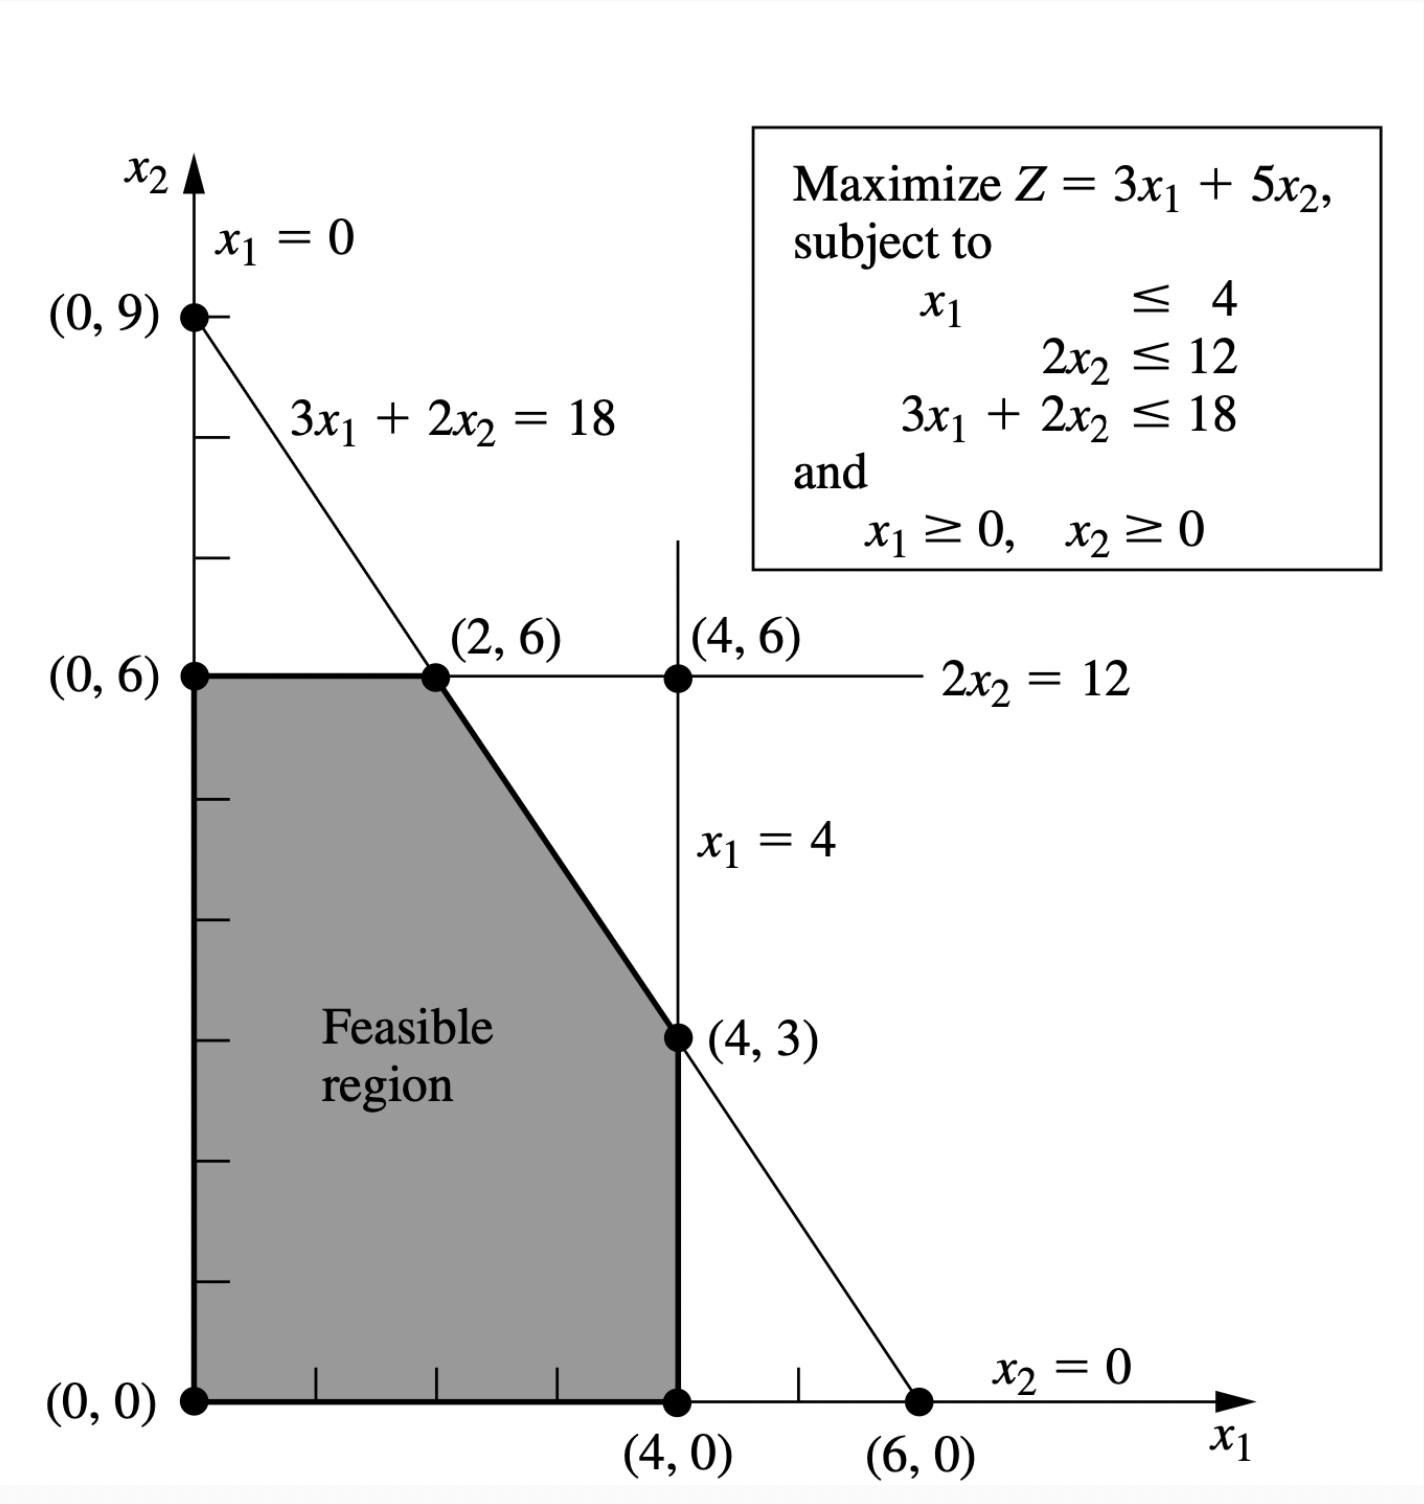
\includegraphics[width=0.5\textwidth]{Frontiera_vincolo_soluzioni_vertice}
    \caption{Frontiera di un vincolo \& Soluzioni di vertice}
    \label{fig:fig1}
\end{figure}

\newpage
\begin{center}
    13 Ottobre 2022
\end{center}
\section{Algoritmo del simplesso}
Nell'algoritmo del simplesso si forniscono le seguenti definizioni:
\begin{itemize}
    \item la \textbf{frontiera} di un vincolo è una linea che forma il confine di ciò che è permesso dal vincolo corrispondente.
    \item i punti di intersezione sono le \textbf{soluzioni di vertice} del problema. Le cinque che si trovano agli angoli della regione ammissibile della Figura \ref{fig:fig1} - (0, 0), (0, 6), (2, 6), (4, 3) e (4, 0) - sono le \textbf{soluzioni ammissibile di vertici} (\textbf{soluzioni CPF}).\\
    Le altre tre - (0, 9), (4, 6) e (6, 0) - sono chiamate soluzioni non ammissibili in un angolo.
\end{itemize}

\noindent
Nell'esempio di Figura \ref{fig:fig1}, ogni soluzione di vertice si trova all'intersezione della frontiera di $2$ vincoli. Per un problema di programmazione lineare con $n$ variabili decisionali, ciascuna delle sue soluzioni di vertice si trova all'intersezione di $n$ frontiere di vincolo.

\vspace{1em}
\subsection{Soluzioni adiacenti}
Alcune coppie di soluzioni CPF  condividono un confine di vincolo, mentre altre coppie non lo condividono. Sarà importante distinguere tra questi casi utilizzando la seguente definizione generale:

% Tabella per le definizione di concetti, etc...
\vspace{1em}
\rowcolors{1}{black!5}{black!5}
\setlength{\tabcolsep}{14pt}
\renewcommand{\arraystretch}{2}
\noindent
\begin{tabularx}{\textwidth}{@{}|P|@{}}
    \hline
    {\textbf{SOLUZIONI ADIACENTI}}\\
    \parbox{\linewidth}{Per qualsiasi problema di programmazione lineare con $n$ variabili decisionali, due \textbf{soluzioni CPF sono adiacenti} se condividono $n - 1$ vincoli.\\
    Le due soluzioni CPF adiacenti sono collegate da un segmento di linea che giace su queste stesse frontiere di vincolo condivise. Tale segmento di linea viene definito \textbf{bordo (spigolo)} della regione ammissibile. \vspace{3mm}}\\
    \hline
\end{tabularx}

\vspace{1em}
\noindent
Posto nell'esempio $n = 2$, due delle sue soluzioni CPF sono adiacenti se condividono un confine di vincolo; ad esempio, (0, 0) e (0, 6) sono adiacenti perché condividono il confine di vincolo $x_1 = 0$, com'è facile vedere dall'immagine:

\begin{figure}[H]
    \centering
    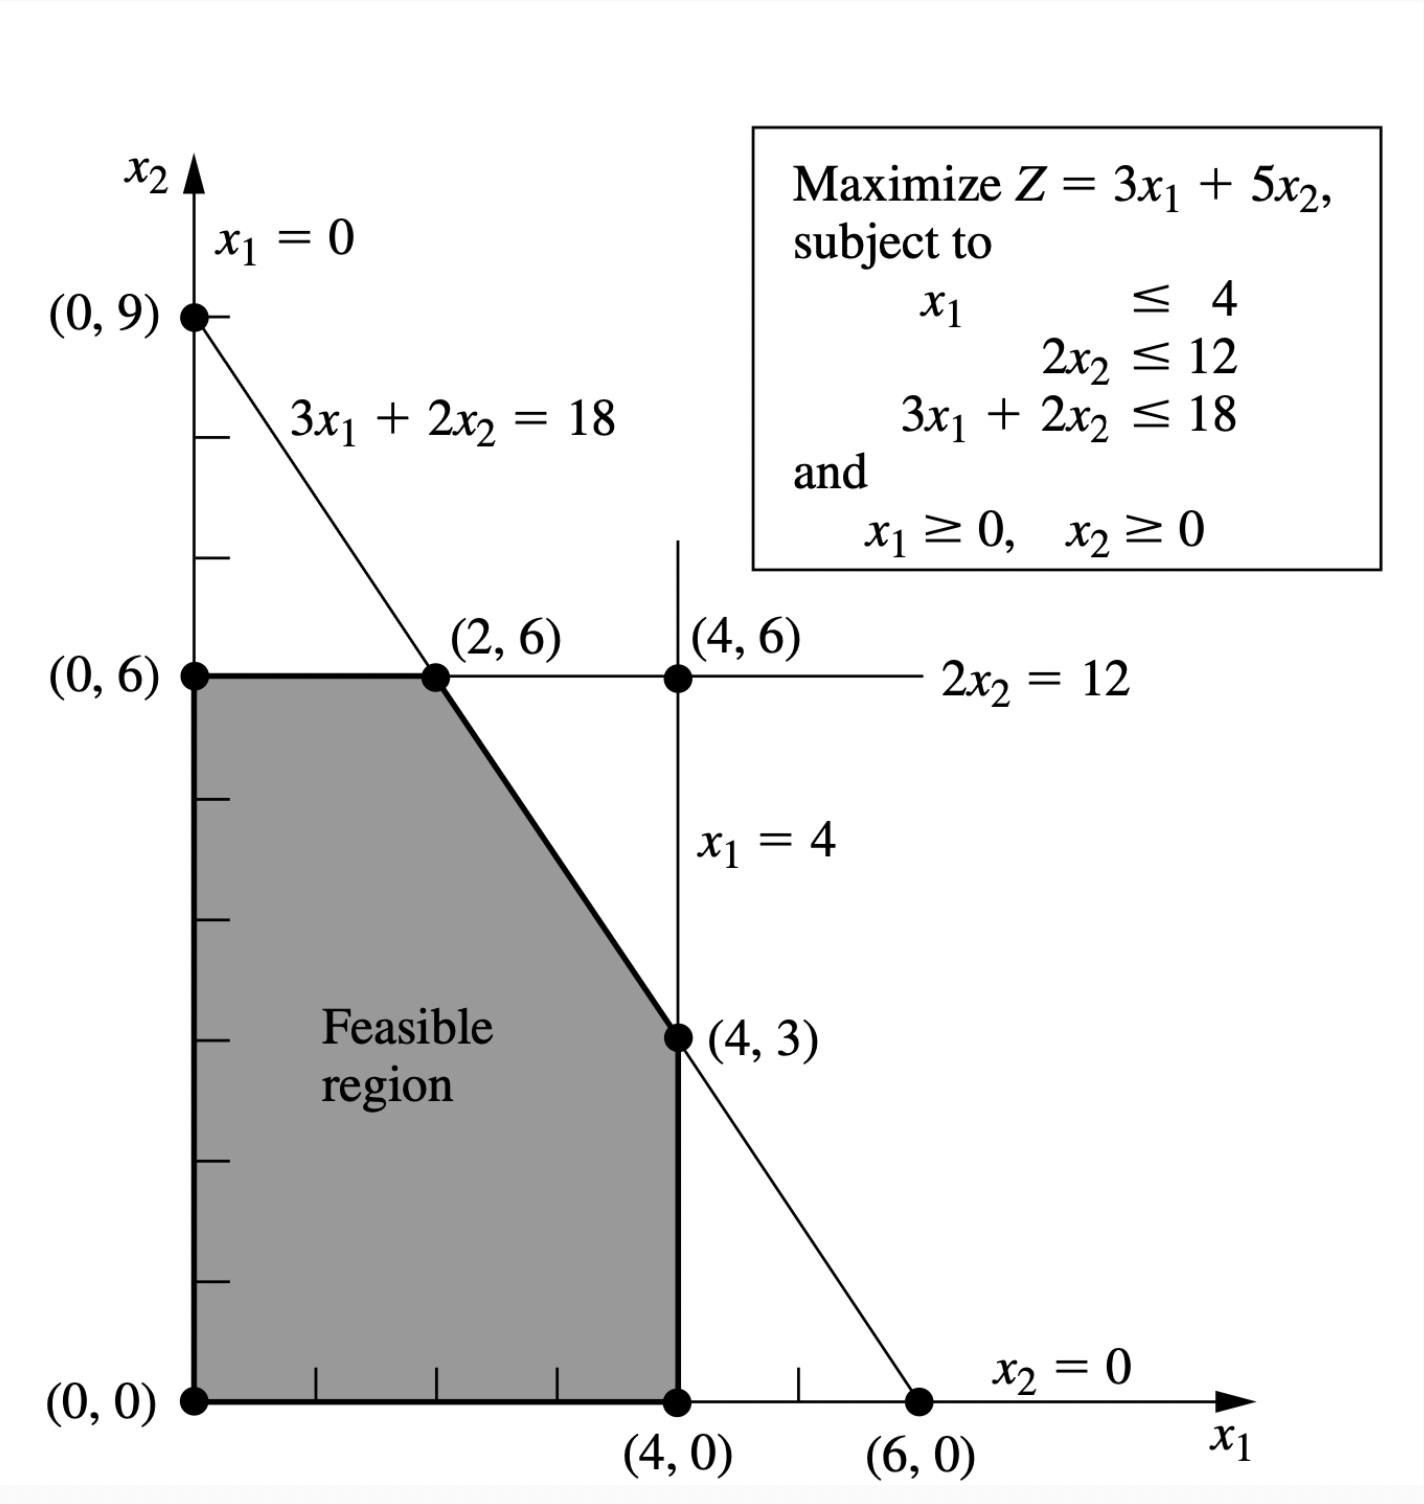
\includegraphics[width=0.5\textwidth]{Frontiera_vincolo_soluzioni_vertice}
    \caption{Frontiera di un vincolo \& Soluzioni di vertice}
    \label{fig:fig1_1}
\end{figure}

\noindent
La regione ammissibile ha cinque spigoli, costituiti dai cinque segmenti di linea che formano il confine di tale regione. Si noti che da ogni soluzione CPF partono due spigoli. Pertanto, ogni soluzione CPF ha due soluzioni CPF adiacenti (ognuna delle quali si trova all'altra estremità di uno dei due spigoli), come elencato nella Tabella \ref{tab:tab1}:

\noindent
\begin{table}[H]
    \rowcolors{1}{white}{white}
    \setlength{\tabcolsep}{8pt}
    \renewcommand{\arraystretch}{1.5}
    \noindent
    \centering
    \begin{tabular}{c|c}
        \hline
        Soluzione CPF & Soluzioni CPF adiacenti\\
        \hline
        (0,0) & (0,6) e (4,0)\\
        (0,6) & (0,0) e (2,6)\\
        (2,6) & (4,3) e (0,6)\\
        (4,3) & (4,0) e (2,6)\\
        (4,0) & (0,0) e (4,3)\\
        \hline
    \end{tabular}
    \caption{Soluzioni CPF adiacenti}
    \label{tab:tab1}
\end{table}   

\vspace{1em}
\subsection{La soluzione ottima in un vertice}
\label{sec:prop1}
Come esposto in precedenza, valgono le seguenti proprietà:

% Tabella per le definizione di concetti, etc...
\vspace{1em}
\rowcolors{1}{black!5}{black!5}
\setlength{\tabcolsep}{14pt}
\renewcommand{\arraystretch}{2}
\noindent
\begin{tabularx}{\textwidth}{@{}|P|@{}}
    \hline
    {\textbf{SOLUZIONE OTTIMA IN UN VERTICE}}\\
    \parbox{\linewidth}{
        \begin{enumerate}
            \item Se esiste esattamente una soluzione ottima, allora deve essere una soluzione CPF.
            \item Se esistono più soluzioni ottime (e una regione ammissibile delimitata), almeno due devono essere soluzioni CPF adiacenti.
        \end{enumerate}
    \vspace{1mm}}\\
    \hline
\end{tabularx}

\vspace{1em}
\noindent
\textbf{Dimostrazione 1}: Per assurdo, si assuma che esista esattamente una soluzione ottima e che non sia una soluzione CPF. Dal momento che, secondo la definizione, una soluzione CPF è una soluzione ammissibile che non si trova su nessun segmento di linea che collega altre due soluzioni ammissibili, dal momento che si è assunto che la soluzione ottima $x^*$ non è una soluzione CPF, ciò implica che devono esistere altre due soluzioni ammissibili tali che il segmento di retta che le unisce contenga la soluzione ottima.\\
I vettori $x'$ e $x''$ denotano tali altre due soluzioni ammissibili e $Z_1$ e $Z_2$ i rispettivi valori della funzione obiettivo. Come ogni altro punto del segmento di retta che collega $x'$ e $x''$
\[x^* = \alpha x'' + (1-\alpha) x'\]
per un valore di $\alpha$ tale che $0 < \alpha < 1$. Pertanto
\[Z^* = \alpha \cdot Z_2 + (1 - \alpha) \cdot Z_1\]
Poiché i pesi $\alpha$ e $1 - \alpha$ sommano a $1$, le uniche possibilità di confronto tra $Z^*$, $Z_1$ e $Z_2$ sono
\begin{enumerate}
    \item $Z^* = Z_1 = Z_2$
    \item $Z_1 < Z^* < Z_2$
    \item $Z_1 > Z^* > Z_2$
\end{enumerate}
La prima possibilità implica che anche $x'$ e $x''$ siano ottimali, il che contraddice l'ipotesi che esista esattamente una soluzione ottimale. Entrambe le ultime possibilità contraddicono l'ipotesi che $x^*$ (che non è una soluzione CPF) sia ottimale. La conclusione che ne deriva è che è impossibile avere un'unica soluzione ottimale che non sia una soluzione CPF.

\vspace{1em}
\noindent
\textbf{Dimostrazione 2}: Ciò che accade quando si risolve graficamente è che la linea della funzione obiettivo continua ad alzarsi finché non contiene il segmento di linea che collega le due soluzioni CPF.\\
La stessa cosa accadrebbe in dimensioni superiori, tranne per il fatto che un iperpiano della funzione obiettivo continuerebbe a essere innalzato fino a contenere il segmento o i segmenti di linea che collegano due (o più) soluzioni CPF adiacenti.\\
Di conseguenza, tutte le soluzioni ottimali possono essere ottenute come medie ponderate di soluzioni CPF ottimali.

\vspace{1em}
\subsection{Numero finito di soluzioni CPF}
Di seguito si espone la proprietà di \textbf{finitezza del numero di soluzioni CPF}:

% Tabella per le definizione di concetti, etc...
\vspace{1em}
\rowcolors{1}{black!5}{black!5}
\setlength{\tabcolsep}{14pt}
\renewcommand{\arraystretch}{2}
\noindent
\begin{tabularx}{\textwidth}{@{}|P|@{}}
    \hline
    {\textbf{FINITEZZA DI SOLUZIONI CPF}}\\
    \parbox{\linewidth}{C'è solo un numero finito di soluzioni CPF. \vspace{3mm}}\\
    \hline
\end{tabularx}

\vspace{1em}
\noindent
Ogni soluzione CPF è la soluzione simultanea di un sistema di $n$ delle $m+n$ equazioni vincolate. Il numero di combinazioni diverse di $m + n$ equazioni prese $n$ alla volta è
\[\binom{m+n}{n} = \frac{(m+n)!}{m! \cdot n!}\]
che è un numero finito.\\
Un'enumerazione esaustiva potrebbe non essere possibile: un problema di programmazione lineare piuttosto piccolo con
solo $m = 50$ e $n = 50$ avrebbe 
\[\frac{100!}{(50!) \cdot 2} \cong 10^{29}\]
sistemi di equazioni da risolvere!\\
Al contrario, il metodo del simplesso (esposto di seguito) dovrebbe esaminare solo circa $100$ soluzioni CPF per un problema di queste dimensioni.

\vspace{1em}
\subsection{La regione ammissibile è convessa}
Di seguito si espone la proprietà di \textbf{convessità della regione ammissibile}:

% Tabella per le definizione di concetti, etc...
\vspace{1em}
\rowcolors{1}{black!5}{black!5}
\setlength{\tabcolsep}{14pt}
\renewcommand{\arraystretch}{2}
\noindent
\begin{tabularx}{\textwidth}{@{}|P|@{}}
    \hline
    {\textbf{CONVESSITÀ DELLA REGIONE AMMISSIBILE}}\\
    \parbox{\linewidth}{Se una soluzione CPF non ha soluzioni CPF adiacenti migliori (misurate da $Z$), allora non esistono soluzioni CPF migliori per la funzione obiettivo: la migliore è quella considerata in principio.\\
    Pertanto, tale soluzione CPF è garantita come soluzione ottimale (dalla proprietà § \ref{sec:prop1}), assumendo solo che il problema possieda almeno una soluzione ottimale (garantita se il problema possiede soluzioni ammissibile e una regione ammissibile limitata). \vspace{3mm}}\\
    \hline
\end{tabularx}

\vspace{1em}
\subsection{Test di ottimalità}
Di seguito si espone il funzionamento del \textbf{test di ottimalità}:

% Tabella per le definizione di concetti, etc...
\vspace{1em}
\rowcolors{1}{black!5}{black!5}
\setlength{\tabcolsep}{14pt}
\renewcommand{\arraystretch}{2}
\noindent
\begin{tabularx}{\textwidth}{@{}|P|@{}}
    \hline
    {\textbf{TEST DI OTTIMALITÀ}}\\
    \parbox{\linewidth}{Dato un qualsiasi problema di programmazione lineare che possieda almeno una soluzione ottimale. Se una soluzione CPF non ha soluzioni CPF adiacenti migliori (misurate da $Z$), allora deve essere una soluzione ottimale. \vspace{3mm}}\\
    \hline
\end{tabularx}

\newpage
\noindent
\textbf{Osservazione}: Quindi, ancora una volta, dato l'esempio seguente

\begin{figure}[H]
    \centering
    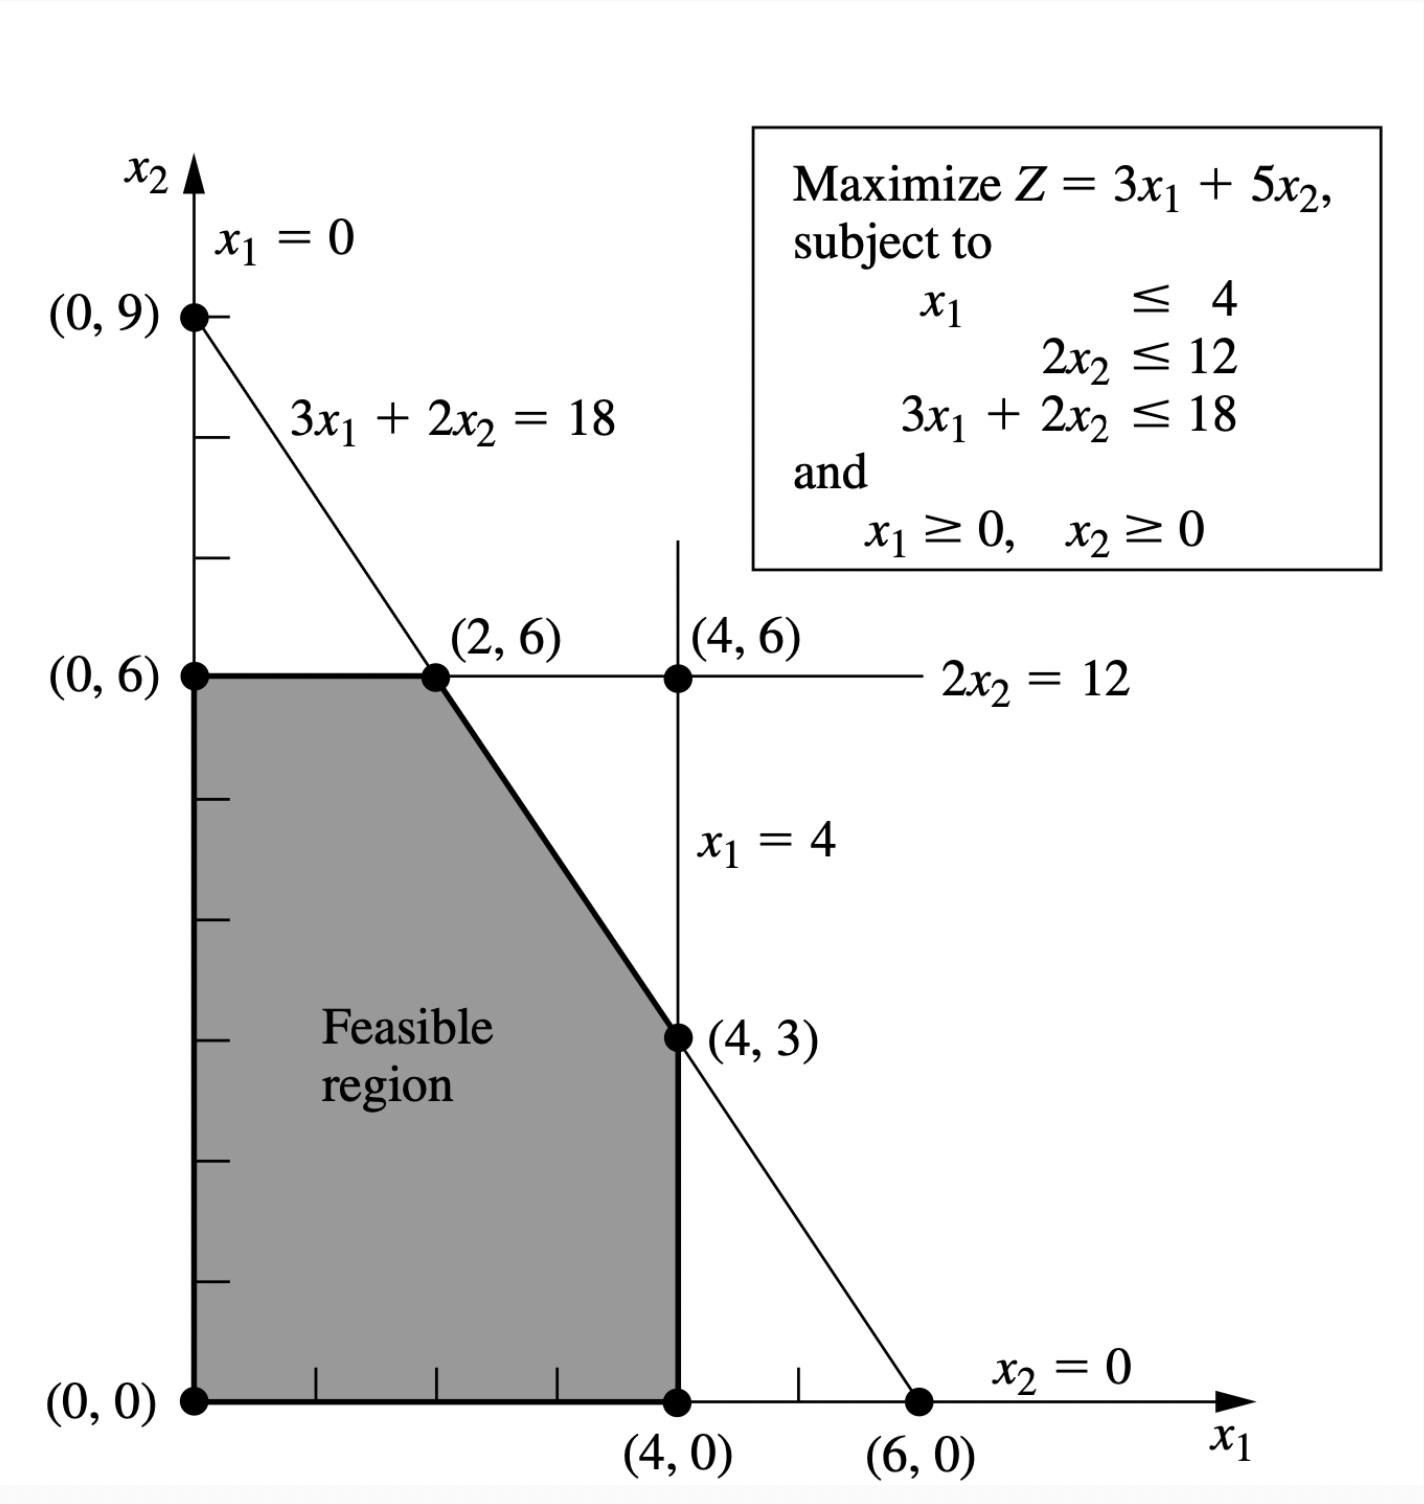
\includegraphics[width=0.5\textwidth]{Frontiera_vincolo_soluzioni_vertice}
    \caption{Frontiera di un vincolo \& Soluzioni di vertice}
    \label{fig:fig1_2}
\end{figure}

\noindent
Il vertice $(2,6)$ deve essere ottimale semplicemente perché il suo corrispondente valore per la funzione obiettivo è $Z=36$ che, ovviamente, è maggiore di $Z=30$ per $(0,6)$ e di $Z=27$ per $(4,3)$. Questo test di ottimalità è quello utilizzato dal metodo del simplesso per determinare quando è stata raggiunta una soluzione ottimale.

\vspace{1em}
\subsection{Algoritmo del simplesso}
Di seguito si espongono i passi dell'\textbf{algoritmo del simplesso}, specificatamente nell'esempio preso in considerazione fino a questo momento:

\begin{itemize}
    \item \textbf{Inizializzazione}: Si sceglie $(0,0)$ come soluzione CPF iniziale da esaminare. Ovviamente $(0,0)$ è una scelta conveniente perché non sono necessari calcoli per identificare tale soluzione CPF.
    \item \textbf{Test di ottimalità}: Si conclude che $(0,0)$ non è una soluzione ottimale, in quanto le soluzioni CPF adiacenti $(4,0)$ e $(0,6)$ sono migliori: per la prima $Z=12$, per la seconda $Z=30$.
    \item \textbf{Iterazione 1}: Si consideri la soluzione CPF adiacente migliore che, in questo caso, è proprio $(0,6)$. Per farlo, si eseguono le tre fasi seguenti:
    \begin{itemize}
        \item Considerando i due bordi della regione ammissibile che partono da $(0,0)$, ci si sposta lungo il bordo che conduce all'asse $x_2$.\\
        Questo perché, con una funzione obiettivo pari a $Z=3x_1 + 5x_2$, l'aumento marginale di $Z$ è maggiore per $x_2$ rispetto ad uno spostamento lungo l'asse $x_1$.
        \item Fermarsi al primo nuovo limite di vincolo, dato da $2x_2 = 12$. Infatti, spostandosi oltre nella direzione selezionata nel passo precedente, si esce dalla regione ammissibile; nell'esempio considerato, spostandosi lungo $x_2$, ma fermandosi al secondo nuovo limite di vincolo, si ottiene $(0,9)$, che è una soluzione non ammissibile in un vertice.
        \item Risolvendo l'intersezione del nuovo insieme di vincoli: $x_1 = 0$ e $2x_2 = 12$ si ottiene immediatamente la soluzione $(0,6)$.
    \end{itemize}
    \item \textbf{Test di ottimalità}: Ancora una volta si conclude che $(0,6)$ non è una soluzione ottimale, in quanto la soluzioni CPF adiacente $(2,6)$ non ancora analizzata (in quanto $(0,0)$ era la soluzione CPF di partenza) è migliore, in quanto $Z=36$.
    \item \textbf{Iterazione 2}: Si consideri la soluzione CPF adiacente migliore che, ossia $(2,6)$. Per farlo, si eseguono le tre fasi seguenti:
    \begin{itemize}
        \item Considerando i due bordi della regione ammissibile che partono da $(0,6)$, si sceglie di spostarsi lungo il bordo che porta a destra, in quanto lo spostamento lungo tale bordo aumenta $Z$, mentre l'indietreggiare lungo l'asse $x_2$ diminuisce $Z$.
        \item Ci si arresta al primo nuovo limite di vincolo incontrato muovendosi in quella direzione: $3x_1 + 2x_2 = 18$. Infatti, spostandosi ulteriormente nella direzione selezionata al passo precedente, si esce dalla regione ammissibile.
        \item Risolvendo l'intersezione del nuovo insieme di vincoli: $3x_1 + 2x_2 = 18$ e $2x_2 = 12$ si ottiene immediatamente la soluzione $(2,6)$.
    \end{itemize}
    \item \textbf{Test di ottimalità}: Infine si conclude che $(2,6)$ è la soluzione ottimale, in quanto nessuna delle soluzioni CPF adiacenti (ossia $(0,6)$ e $(4,3)$) è migliore: per la prima $Z=30$, per la seconda $Z=27$.
\end{itemize}

\vspace{1em}
\noindent
\subsection{Relazione tra soluzioni ottimali e CPF}
Di seguito si espone la \textbf{relazione tra soluzioni ottimali e CPF}:

% Tabella per le definizione di concetti, etc...
\vspace{1em}
\rowcolors{1}{black!5}{black!5}
\setlength{\tabcolsep}{14pt}
\renewcommand{\arraystretch}{2}
\noindent
\begin{tabularx}{\textwidth}{@{}|P|@{}}
    \hline
    {\textbf{RELAZIONE TRA SOLUZIONI OTTIMALI E CPF}}\\
    \parbox{\linewidth}{Il metodo del simplesso si concentra esclusivamente sulle soluzioni CPF. Per qualsiasi problema che abbia almeno una soluzione ottimale, per trovarla è sufficiente trovare la migliore soluzione CPF. \vspace{3mm}}\\
    \hline
\end{tabularx}

\vspace{1em}
\noindent
\textbf{Osservazione}: Poiché il numero di soluzioni fattibili è generalmente infinito, la riduzione del numero di soluzioni da esaminare a un piccolo numero finito (solo tre nell'esempio considerato) rappresenta un'enorme semplificazione.

\vspace{1em}
\subsection{Flusso del metodo del simplesso}
Il metodo del simplesso è un algoritmo iterativo con la seguente struttura:
\begin{itemize}
    \item Configurare l'algoritmo andando a determinare una prima soluzione CPF ammissibile;
    \item Se la soluzione CPF è ottimale, ci si arresta. Altrimenti si prosegue con un'ulteriore iterazioni fino a trovare una migliore soluzione CPF.
\end{itemize}
Per la risoluzione dell'esempio risolto, tale diagramma di flusso è stato seguito attraverso due iterazioni fino a trovare una soluzione ottimale.

\vspace{1em}
\noindent
\subsection{Inizializzazione dell'algoritmo del simplesso}
Di seguito si espone il concetto chiave di \textbf{inizializzazione dell'algoritmo del simplesso}:

% Tabella per le definizione di concetti, etc...
\vspace{1em}
\rowcolors{1}{black!5}{black!5}
\setlength{\tabcolsep}{14pt}
\renewcommand{\arraystretch}{2}
\noindent
\begin{tabularx}{\textwidth}{@{}|P|@{}}
    \hline
    {\textbf{INIZIALIZZAZIONE DELL'ALGORITMO DEL SIMPLESSO}}\\
    \parbox{\linewidth}{Quando possibile, per l'inizializzazione dell'algoritmo del simplesso, si sceglie l'origine $(0,0)$, ponendo tutte le variabili decisionali pari a $0$ come soluzione CPF iniziale.\\
    Infatti, quando le variabili decisionali sono troppe per trovare una soluzione CPF iniziale graficamente, tale scelta elimina la necessità di utilizzare procedure algebriche per trovare e risolvere una prima soluzione CPF. \vspace{3mm}}\\
    \hline
\end{tabularx}

\vspace{1em}
\noindent
\textbf{Osservazione}: La scelta dell'origine è comunemente possibile quando tutte le variabili decisionali hanno vincoli di non negatività, perché l'intersezione dei confini di questi vincoli produce l'origine come soluzione angolare: tale soluzione è quindi una soluzione CPF, a meno che non sia inaffrontabile perché viola uno o più vincoli.\\
Se non è ammissibile, sono necessarie procedure speciali per trovare la soluzione CPF iniziale: in particolare, nel caso in cui $(0,0)$ non sia una soluzione ammissibile, si creerà un problema alternativo, forzando $(0,0)$ come vertice ammissibile iniziale, tramite l'individuazione di variabili artificiali.

\vspace{1em}
\subsection{Scelta di una soluzione CPF migliore ad ogni iterazione}
Di seguito si espone la logica alla base della \textbf{scelta di una soluzione CPF migliore ad ogni iterazione}:

% Tabella per le definizione di concetti, etc...
\vspace{1em}
\rowcolors{1}{black!5}{black!5}
\setlength{\tabcolsep}{14pt}
\renewcommand{\arraystretch}{2}
\noindent
\begin{tabularx}{\textwidth}{@{}|P|@{}}
    \hline
    {\textbf{SCELTA DEL MIGLIORE VERTICE CPF AD OGNI ITERAZIONE}}\\
    \parbox{\linewidth}{Data una soluzione CPF, è molto più veloce, dal punto di vista computazionale, raccogliere informazioni sulle \textbf{soluzioni CPF adiacenti} che sulle altre soluzioni CPF.\\
    Pertanto, ogni volta che l'algoritmo del simplesso esegue un'iterazione per passare dalla soluzione CPF corrente ad una migliore, si sceglie \textbf{sempre} una \textbf{soluzione CPF adiacente} a quella corrente, escludendo altre soluzioni CPF; di conseguenza, l'intero percorso seguito per raggiungere una soluzione ottimale è \textbf{lungo i bordi della regione ammissibile}.\\
    Dopo aver identificato la soluzione CPF corrente, l'algoritmo del simplesso esamina ciascuno degli spigoli della regione ammissibile che si diramano da questa soluzione CPF e identifica il tasso di miglioramento per $Z$ che si otterrebbe spostandosi lungo tale spigolo. Tra gli spigoli con un tasso di miglioramento positivo per $Z$, si sceglie quindi di spostarsi lungo quello con il tasso di miglioramento maggiore per $Z$.\\
    L'iterazione viene, dunque, completata risolvendo prima la soluzione CPF adiacente all'altra estremità di questo spigolo e poi considerando tale nuova soluzione CPF adiacente come soluzione CPF corrente per il test di ottimalità e (se necessario) per l'iterazione successiva.\vspace{3mm}}\\
    \hline
\end{tabularx}

\vspace{1em}
\noindent
\textbf{Osservazione}: Riprendendo in considerazione l'esempio di partenza:

\begin{figure}[H]
    \centering
    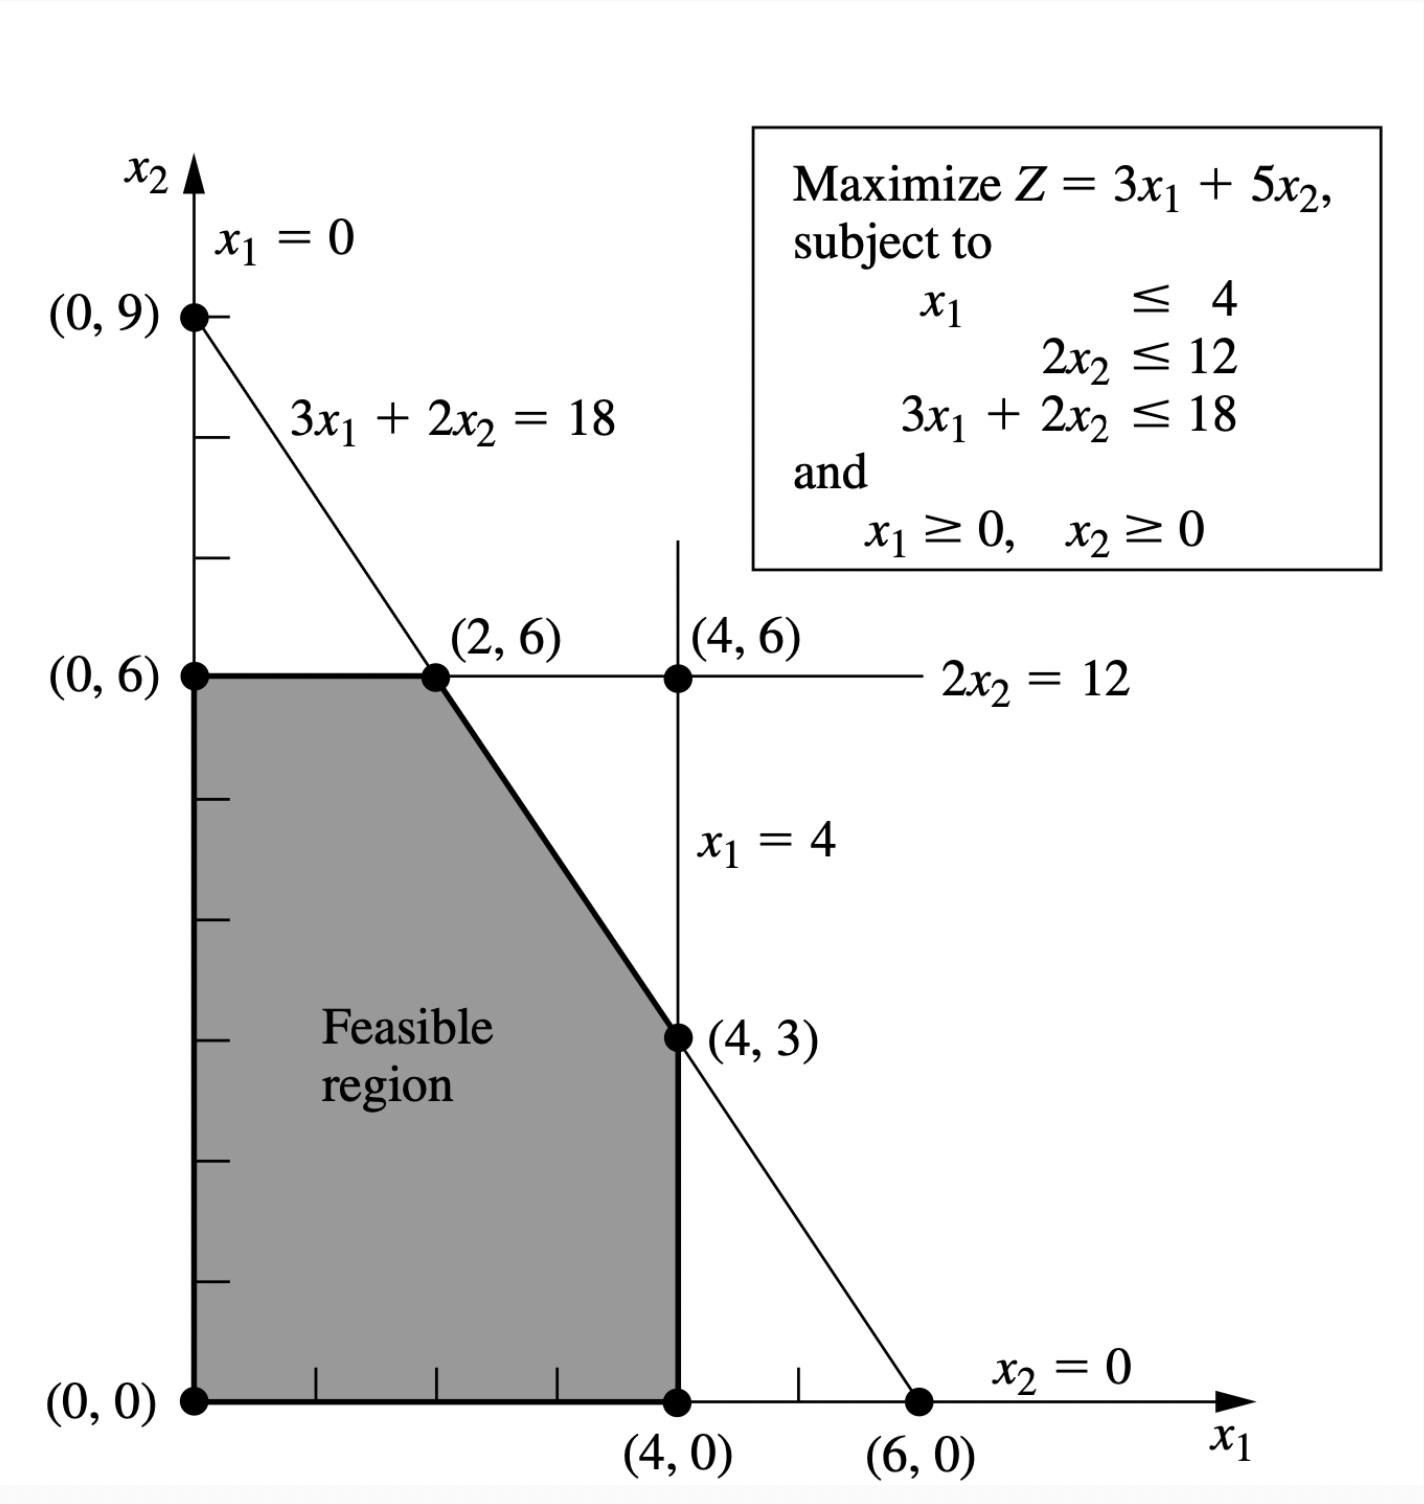
\includegraphics[width=0.5\textwidth]{Frontiera_vincolo_soluzioni_vertice}
    \caption{Frontiera di un vincolo \& Soluzioni di vertice}
    \label{fig:fig1_3}
\end{figure}

\vspace{1em}
\noindent
\textbf{Osservazione 1}: Nella prima iterazione, spostandosi da $(0,0)$ lungo il bordo sull'asse $x_1$ si otterrebbe un tasso di miglioramento di $Z$ pari a $3$, in quanto
\[\frac{\partial Z}{\partial x_1} = 3\]
per cui $Z$ aumenta di $3$ per ogni aumento unitario di $x_1$, mentre spostandosi lungo il bordo sull'asse $x_2$ si otterrebbe un tasso di miglioramento di $Z$ pari a $5$, in quanto
\[\frac{\partial Z}{\partial x_2} = 5\]
per cui $Z$ aumenta di $5$ per ogni aumento unitario di $x_2$; da tale evidenza è facile decidere di spostarsi lungo quest'ultimo bordo.\\
Alla seconda iterazione, invece, l'unico bordo che si dirama da $(0,6)$ e che produce un tasso di miglioramento positivo in $Z$ è il bordo che porta a $(2,6)$, per cui si decide di spostarsi lungo tale bordo.

\vspace{1em}
\noindent
\textbf{Osservazione 2}: Tuttavia, non è sempre garantito a priori che sia una buona strada quella di spostarsi lungo il bordo con il maggior tasso di miglioramento per $Z$.\\
Pertanto, in generale, tutte le scelte sono arbitrarie ed ugualmente valide, dal punto di vista della correttezza, ma non dell'efficienza.

\vspace{1em}
\subsection{Eseguire il test di ottimalità efficacemente}
Di seguito si espone il metodo con cui eseguire il \textbf{test di ottimalità efficacemente}:

% Tabella per le definizione di concetti, etc...
\vspace{1em}
\rowcolors{1}{black!5}{black!5}
\setlength{\tabcolsep}{14pt}
\renewcommand{\arraystretch}{2}
\noindent
\begin{tabularx}{\textwidth}{@{}|P|@{}}
    \hline
    {\textbf{TEST DI OTTIMALITÀ EFFICACE}}\\
    \parbox{\linewidth}{Un tasso di miglioramento positivo per la funzione obiettivo $Z$ implica che la soluzione CPF adiacente sia migliore della soluzione CPF corrente, mentre un tasso di miglioramento negativo in $Z$ implica che la soluzione CPF adiacente sia peggiore.\\
    Pertanto, il test di ottimalità consiste semplicemente nel verificare se uno qualsiasi degli spigoli produce un tasso di miglioramento positivo per $Z$. Se nessuno di essi lo dà, allora la soluzione CPF attuale è ottimale.\vspace{3mm}}\\
    \hline
\end{tabularx}

\vspace{1em}
\noindent
\textbf{Osservazione 1}: Nell'esempio considerato, infatti, spostandosi lungo uno dei due bordi che si diramano da $(2,6)$, il valore della funzione obiettivo $Z$ diminuisce. Poiché le richieste del problema prevedono di massimizzare $Z$, questo fatto porta immediatamente alla conclusione che $(2,6)$ è ottimale.

\vspace{1em}
\noindent
\textbf{Osservazione 2}: Il vertice CPF $(2,6)$ è il punto di intersezione tra $2x_2 = 12$ (cioè $x_2 = 6$) e $3x_1 + 2x_2 = 18$; quest'ultimo vincolo può anche essere scritto come
\[x_1 = 6 - \frac{2}{3}x_2\]
Quindi, quando $Z = 3x_1 + 5x_2$ si muove lungo tale vincolo, si ha che 
\[Z = 3 \cdot \left(6-\frac{2}{3}\right)x_2+5x_2 \hspace{1em} \rightarrow \hspace{1em} Z = 18+3x_2\]
Se $x_2 = 6$, pertanto, si ottiene che $Z = 36$. Quindi, se $x_2 < 6$, $Z$ diminuisce e quindi non è un'opzione praticabile. Poiché anche spostarsi lungo $x_2 = 6$ non consente di aumentare $Z$, ne consegue che (2, 6) è la soluzione ottimale.\\
Analogamente, se si considera
\[x_2 = 9 - \frac{3}{2}x_1 \hspace{1em} \text{allora} \hspace{1em} Z = 45 - \frac{9}{2} x_1\]
per cui in $x_1 = 2$, $Z = 36$ e tale valore diminuisce finché $x_1$ aumenta.

\vspace{1em}
\noindent
\textbf{Esercizio}: Un ragionamento analogo può essere eseguito ponendo come funzione obiettivo $Z = 3x_1 + x_2$. In questo caso si osserverà che (2, 6) non è ottimale.

\newpage
\begin{center}
    14 Ottobre 2022
\end{center}
È noto che la soluzione ottima si trova sempre su un vertice. Secondo l'algoritmo del simplesso, in particolare, partendo da un vertice della regione ammissibile, ci si sposta verso un vertice adiacente, senza analizzare tutti i vertici ammissibili, necessariamente, in modo tale da massimizzare la funzione obiettivo.
Per la convessità della regione ammissibile, ogni qualvolta ci si sposta da un vertice ad un altro adiacente, e il valore della funzione obiettivo non migliora, allora la soluzione CPF considerata in principio è quella ottimale.

\vspace{1em}
\subsection{Forma standard e soluzioni di base}
Un qualunque problema di programmazione lineare può sempre essere espresso in \textbf{forma standard}, come segue
\begin{align*}
    \max z = c x\\
    A x = b (b \geq 0)\\
    x \geq 0
\end{align*}
Pertanto, dato un problema formulato come sopra, posto il $rg(A)=m$, ossia il numero di colonne linearmente indipendenti della matrice $A$ è $m$. Giacché $m < n$, eventualmente riordinando le colonne, si può porre
\[A = \left[B \vert N\right]\]
in cui
\begin{itemize}
    \item $B$ è una matrice quadrata non singolare $m \times m$ detta \textbf{matrice delle colonne in base};
    \item $N$ è una matrice $m \times (n-m)$ detta \textbf{matrice delle colonne fuori base};
\end{itemize}
La matrice $B$ è composta da $m$ colonne di $A$ linearmente indipendenti che formano una base nello spazio vettoriale ad $m$ dimensioni delle colonne di $A$.\\
In corrispondenza di una scelta di $B$ ed $N$ si può partizionare anche il vettore delle $x$, ottenendo
\[x = \left[
    \rowcolors{1}{white}{white}
    \begin{array}{c}
        x_B\\
        x_N
    \end{array}
\right] 
\rowcolors{1}{white}{white}
\begin{array}{l}
    \text{con } m \text{ componenti}\\
    \text{con } m-n \text{ componenti}\\
\end{array}\]
in cui
\begin{itemize}
    \item $x_B$ è detto \textbf{vettore delle variabili in base} (\textbf{vettore di base});
    \item $x_N$ è detto \textbf{vettore delle variabili fuori base}.
\end{itemize}
Il sistema di equazioni lineari $Ax = b$ si può riscrivere come
\[\left[B \vert N\right] \cdot \left[
    \rowcolors{1}{white}{white}
    \begin{array}{c}
        x_B\\
        x_N
    \end{array}
\right] = b \hspace{1em} \rightarrow \hspace{1em} B x_B + N x_N = b\]
Moltiplicando per l'inversa della matrice delle colonne in base $B$, si ottiene
\[\boxed{x_B = B^{-1}b - B^{-1}N x_N}\]
Per ogni base $B$ ogni soluzione del sistema $Ax = b$ corrisponde a determinare il valore per $m$ variabili $x_B$ avendo fissato arbitrariamente il valore per le restanti $n-m$ variabili $x_N$.\\
Una scelta particolarmente importante è porre $x_N=0$, da cui si ottiene la corrispondente soluzione di base
\[x=\left[
    \rowcolors{1}{white}{white}
    \begin{array}{c}
        x_B\\
        x_N
    \end{array}
\right]=\left[
    \rowcolors{1}{white}{white}
    \begin{array}{c}
        B^{-1} b\\
        0
    \end{array}
\right]\]
per cui se $B^{-1}b \geq 0$ si ottiene una soluzione di base ammissibile (BFS) per il sistema
\[Ax = b, \hspace{1em} x \geq 0\]

\vspace{1em}
\subsection{Vertici e BFS}
Si espone di seguito un importante considerazione in merito alla relazione tra \textbf{vertici e BFS}:

% Tabella per le definizione di concetti, etc...
\vspace{1em}
\rowcolors{1}{black!5}{black!5}
\setlength{\tabcolsep}{14pt}
\renewcommand{\arraystretch}{2}
\noindent
\begin{tabularx}{\textwidth}{@{}|P|@{}}
    \hline
    {\textbf{VERTICI E BFS}}\\
    \parbox{\linewidth}{Dato il problema $Ax = b, x \geq 0$, una soluzione $x$ è un vertice del poliedro $P(A, b)$ \textbf{se e solo se} $x$ è una BFS.\\
    Questo perché un punto di un poliedro è un vertice (punto estremo) se e solo se soddisfa all'uguaglianza $n$ vincoli linearmente indipendenti, quindi basta dimostrare che ogni BFS soddisfa $n$ vincoli linearmente indipendenti tra $Ax = b, x \geq 0$.\\
    Per definizione ogni BFS soddisfa all'uguaglianza ($n-m$) vincoli $x \geq 0$ e gli $m$ vincoli di $Ax = b$. I vincoli stringenti sono linearmente indipendenti poiché la matrice dei loro coefficienti è certamente non singolare essendo della forma
    \[\left(
            \begin{array}{cc}
                B & N\\
                0 & I_{n-m}
            \end{array}
    \right)\]
    \vspace{-1mm}}\\
    \hline
\end{tabularx}

\vspace{2em}
\noindent
\textbf{Esempio}: Si consideri il seguente problema, così formulato:
\begin{align*}
    \max z = 2 x_1 + x_2\\
    x_1+x_2 \leq 5\\
    -x_1+x_2 \leq 0\\
    6x_1 + 2x_2 \leq 21\\
    x_1,x_2 \geq 0
\end{align*}
Tale sistema non è in forma standard, ma espresso solo in termini delle variabili strutturali (cioè quelle che hanno un immediata corrispondenza fisica col sistema reale che viene modellato).\\
Per manipolarlo opportunamente, lo si trasforma in forma standard introducendo le \textbf{variabili di slack} $x_3$, $x_4$, $x_5$, ottenendo
\begin{align*}
    \max z = 2 x_1 + x_2\\
    x_1+x_2+x_3=5\\
    -x_1+x_2+x_4=0\\
    6x_1 + 2x_2+x_5=21\\
    x_1,x_2,x_3,x_4,x_5 \geq 0
\end{align*}
in cui è essenziale capire che le variabili di slack sono sempre \textbf{non negative}, per dei vincoli di $\leq$. È fondamentale ciò, perché se fossero negative, significherebbe, nel caso della prima diseguaglianza, per esempio, che $x_1+x_2 \geq 5$, che contraddice il vincolo di partenza.\\
Per ogni vincolo $\leq$, pertanto, si deve introdurre una variabile di slack non negativa. Ecco che ora si è trasformato il problema in forma standard, per cui
\[A = \left[
    \rowcolors{1}{white}{white}
    \begin{array}{ccccc}
        1 & 1 & 1 & 0 & 0\\
        -1 & 1 & 0 & 1 & 0\\
        6 & 2 & 0 & 0 & 1
    \end{array}
\right] \hspace{1em} \text{e} \hspace{1em} b = \left[
    \rowcolors{1}{white}{white}
    \begin{array}{c}
        5\\
        0\\
        21
    \end{array}
\right]\]
Per individuare i vertici, avendo $n=5$ variabili e $m=3$ vincoli, si pongono a $0$ due variabili (le cosiddette \textbf{variabili fuori base}) in tutti i modi possibili, ottenendo un sistema di equazioni con $m=3$ equazioni e $3$ incognite che è risolubile e, non solo, la soluzione è un punto, ossia il vertice cercato.

\vspace{1em}
\noindent
\textbf{Esercizio}: Si pongano a $0$ le variabili $x_4,x_5$ di slack, considerando
\[x_N = \left[
    \rowcolors{1}{white}{white}
    \begin{array}{c}
        x_4\\
        x_5
    \end{array}
\right] = 0\]
Ciò porta a dover determinare
\[x_B = \left[
    \rowcolors{1}{white}{white}
    \begin{array}{c}
        x_1\\
        x_2\\
        x_3
    \end{array}
\right] = B^{-1} \cdot b\]
Giacché $B$ è la matrice quadrata dei corrispondenti vettori dei coefficienti per $x_1$, $x_2$ e $x_3$, si ottiene, dalla matrice $A$ di partenza
\[B = \left[
    \rowcolors{1}{white}{white}
    \begin{array}{ccc}
        1 & 1 & 1\\
        -1 & 1 & 0\\
        6 & 2 & 0
    \end{array}
\right]\]
Per invertire tale matrice, se ne calcola il determinante e la matrice dei cofattori, per cui
\[\det(B) = -1 \cdot 2 - 6 \cdot 1 = -8 \hspace{1em} \text{e} \hspace{1em} \text{cof} B = \left[
    \rowcolors{1}{white}{white}
    \begin{array}{ccc}
        0 & 0 & -8\\
        2 & -6 & 4\\
        -1 & -1 & 2
    \end{array}
\right]\]
per cui la matrice inversa cercata è
\[B^{-1} = \frac{1}{\det(B)} \cdot \text{cof}^{t}(B) = \frac{1}{8} \cdot \left[
    \rowcolors{1}{white}{white}
    \begin{array}{ccc}
        0 & 2 & -1\\
        0 & -6 & -1\\
        -8 & 4 & 2
    \end{array}
\right]
\]
pertanto si può ottenere il vettore $x_B$ come segue
\[x_B=B^{-1} \cdot b = \frac{1}{\det(B)} \cdot \text{cof}^{t}(B) = \frac{1}{8} \cdot \left[
    \rowcolors{1}{white}{white}
    \begin{array}{ccc}
        0 & 2 & -1\\
        0 & -6 & -1\\
        -8 & 4 & 2
    \end{array}
\right] \cdot \left[
    \rowcolors{1}{white}{white}
    \begin{array}{c}
        5\\
        0\\
        21
    \end{array}
\right] = \left[
    \rowcolors{1}{white}{white}
    \begin{array}{c}
        \dfrac{21}{8}\\
        \dfrac{21}{8}\\
        -\dfrac{1}{4}\\
    \end{array}
\right]\]
Tuttavia, tale soluzione non risulta ammissibile in quanto si è ottenuto vettore con componenti non tutte $\geq 0$, come richiesto dai vincoli.

\vspace{1em}
\noindent
\textbf{Osservazione}: Attenzione che, con questo approccio, si individuano tutti i vertici possibili, pari a
\[\binom{n}{n-m} = \frac{n!}{m! \cdot (n-m)!}\]
Tuttavia non è detto che siano tutte ammissibili, in quanto per essere un vertice ammissibile deve soddisfare tutti i vincoli del problema. Non solo, ma è anche possibile che con questo metodo si individui un numero di vertici ammissibile maggiore del numero effettivo dei vertici, in quanto uno stesso vertice può essere intersezione di più di due vincoli.\\
Per esempio, nel caso di una prima intersezione, denotata con $P_1$, le variabili poste a $0$ sono $x_1$, $x_2$ e $x_4$, per cui le coppie di vincoli che producono come intersezione $P_1$ sono $x_1$ e $x_2$, $x_1$ e $x_4$, $x_2$ e $x_4$, per un totale di
\[\binom{3}{2}=3\]
Pertanto, siccome il limite superiore delle possibili basi è
\[\binom{n}{n-m} = \binom{5}{2} = 10\]
non tutte le basi corrispondono ad una soluzione ammissibile BFS, ma solamente $6$ sono ammissibili. Siccome i vertici sono $4$, vi saranno BFS \textbf{degeneri}.

\vspace{1em}
\subsection{Variabili di surplus}
Se in un problema di programmazione lineare vi sono dei vincoli di $\geq$, per trasformare il problema in forma standard si introducono delle \textbf{variabili di surplus} con segno opposto, ad esempio
\[-3x_1 + 2x_2 \geq 5 \hspace{1em} \rightarrow \hspace{1em} -3x_1 + 2x_2 - x_6 = 5\]
in modo tale da rispettare il vincolo di $\geq 0$ di partenza.

\vspace{1em}
\subsection{Funzione obiettivo in forma matriciale}
Esplicitando la funzione obiettivo
\[z = c x = \left[c_B \cdot c_N\right] \cdot \left[
\rowcolors{1}{white}{white}
\begin{array}{c}
    x_b\\
    x_N
\end{array}
\right] = c_B x_B + c_N x_N 
\]
e sostituendo a $x_B$ la forma ottenuta in precedenza, ossia
\[x_B = B^{-1} b - B^{-1} N x_N\]
si ottiene
\[z=c_B B^{-1}b - \left(c_B B^{-1}N - c_N\right) \cdot x_N\]
per cui il valore dell'obiettivo corrispondente alla base $B$ è quindi
\[\boxed{Z(B) = c_B B^{-1} b}\]

\newpage
\begin{center}
    17 Ottobre 2022
\end{center}
\textbf{Esercizio 1}: Si consideri il seguente problema di programmazione lineare, così formalizzato
\begin{align*}
    &\max z = 2x_1+x_2\\
    &x_2 \leq 10\\
    &2x_1+5x_2 \leq 60\\
    &x_1+x_2 \leq 18\\
    &3x_1+x_2 \leq 44\\
    &x_1 \geq 0, x_2 \geq 0
\end{align*}
Allora si rappresenti sul diagramma seguente la regione ammissibile, considerando $x_1$ in ascissa e $x_2$ in ordinata

\begin{figure}[H]
    \pgfplotsset{compat = newest}
    \begin{tikzpicture}
 
        \begin{axis}[
            xmin = 0, xmax = 21,
            ymin = 0, ymax = 21,
            xtick distance = 3,
            ytick distance = 5,
            grid = both,
            minor tick num = 1,
            major grid style = {lightgray},
            minor grid style = {lightgray!25},
            width = \textwidth,
            height = 0.5\textwidth]
            \addplot[
                name path global=vin1,
                domain = 0:30,
                samples = 200,
                smooth,
                thick,
                red,
            ] {10};
            \addplot[
                name path global=vin2,
                domain = 0:30,
                samples = 200,
                smooth,
                thick,
                blue,
            ] {12-2/5*x};
            \addplot[
                name path global=vin3,
                domain = 0:30,
                samples = 200,
                smooth,
                thick,
                orange,
            ] {18-x};
            \addplot[
                name path global=vin4,
                domain = 0:30,
                samples = 200,
                smooth,
                thick,
                green,
            ] {44-3*x};
            \fill[name intersections={of=vin1 and vin2,by=point1},
            name intersections={of=vin2 and vin3,by=point2},
            name intersections={of=vin3 and vin4,by=point3},
            ][very thick,draw=orange,pattern=crosshatch dots,pattern color=green!60!white] (0,0)--(0,10)--(point1)--(point2)--(point3)--(14.7,0)--(0,0);
            \coordinate[label=above:$A$] (A) at ([yshift=+1.5mm]point1);
            \coordinate[label=above:$B$] (B) at ([yshift=+1.5mm]point2);
            \coordinate[label=above:$C$] (C) at ([yshift=+1.5mm]point3);
            \node at (point1)[violet!50,circle,fill,inner sep=-0.5pt]{$A$};
            \node at (point2)[violet!50,circle,fill,inner sep=-0.5pt]{$B$};
            \node at (point3)[violet!50,circle,fill,inner sep=-0.5pt]{$C$};
        \end{axis}
        \end{tikzpicture}
\end{figure}

\vspace{1em}
\noindent
\textbf{Esercizio 3}: Si consideri il seguente problema di programmazione lineare
\begin{align*}
    &\max z = 5x_1+2x_2\\
    &2x_1-x_2 \leq -1\\
    &-x_1+2x_2 \leq -1\\
    &x_1 \geq 0, x_2 \geq 0
\end{align*}
La rappresentazione grafica produce il risultato seguente:

\begin{figure}[H]
    \pgfplotsset{compat = newest}
    \begin{tikzpicture}
 
        \begin{axis}[
            xmin = 0, xmax = 21,
            ymin = 0, ymax = 21,
            xtick distance = 3,
            ytick distance = 5,
            grid = both,
            minor tick num = 1,
            major grid style = {lightgray},
            minor grid style = {lightgray!25},
            width = \textwidth,
            height = 0.5\textwidth]
            \addplot[
                name path global=xdown,
                domain = 0:30,
                samples = 200,
                smooth,
                very thin,
                black,
            ] {0};
            \addplot[
                name path global=y21,
                domain = 0:30,
                samples = 200,
                smooth,
                very thin,
                black,
            ] coordinates {(21,0)(21,21)};
            \addplot[
                name path global=xtop,
                domain = 0:30,
                samples = 200,
                smooth,
                very thin,
                black,
            ] {21};
            \addplot[
                name path global=y0,
                domain = 0:30,
                samples = 200,
                smooth,
                very thin,
                black,
            ] coordinates {(0,0)(0,21)};
            \addplot[
                name path global=vin1,
                domain = 0:30,
                samples = 200,
                smooth,
                thick,
                red,
            ] {1+2*x};
            \addplot[
                name path global=vin2,
                domain = 0:30,
                samples = 200,
                smooth,
                thick,
                blue,
            ] {-1/2+1/2*x};
        \end{axis}
        \fill[name intersections={of=vin1 and y0,by=point1},
            name intersections={of=y0 and xtop,by=point2},
            name intersections={of=vin1 and xtop,by=point3},
            ][very thick,draw=orange,pattern=crosshatch dots,pattern color=green!60!white] ([yshift=-1.5mm]point1)--([yshift=-1.5mm]point2)--([yshift=-1.5mm]point3)--([yshift=-1.5mm]point1);

        \fill[name intersections={of=vin2 and xdown,by=point1},
            name intersections={of=vin2 and y21,by=point2},
            name intersections={of=y21 and xdown,by=point3},
            ][very thick,draw=cyan,pattern=crosshatch dots,pattern color=magenta!60!white] ([yshift=-1.5mm]point1)--([yshift=-1.5mm]point2)--([yshift=-1.5mm]point3)--([yshift=-1.5mm]point1);
        \end{tikzpicture}
\end{figure}

% Importante per capire qual'è la regione ammissibile: verificare se (0,0) soddisfa la disequazione del vincolo
% Importante per capire la direzione della funzione obiettivo: a seconda della massimizzazione o minimizzazione e dei segni di x_1 e x_2

\vspace{1em}
\noindent
\textbf{Esercizio 4}: Si consideri il seguente problema di programmazione lineare
\begin{align*}
    &\min z = 40x_1+50x_2\\
    &2x_1+3x_2 \geq 30\\
    &x_1+x_2 \geq 12\\
    &2x_1+x_2 \geq 20\\
    &x_1 \geq 0, x_2 \geq 0
\end{align*}
La rappresentazione grafica produce il risultato seguente:

\begin{figure}[H]
    \pgfplotsset{compat = newest}
    \begin{tikzpicture}
 
        \begin{axis}[
            xmin = 0, xmax = 16,
            ymin = 0, ymax = 21,
            xtick distance = 3,
            ytick distance = 5,
            grid = both,
            minor tick num = 1,
            major grid style = {lightgray},
            minor grid style = {lightgray!25},
            width = \textwidth,
            height = 0.5\textwidth]
            \addplot[
                name path global=xdown,
                domain = 0:30,
                samples = 200,
                smooth,
                very thin,
                black,
            ] {0};
            \addplot[
                name path global=y21,
                domain = 0:30,
                samples = 200,
                smooth,
                very thin,
                black,
            ] coordinates {(21,0)(21,21)};
            \addplot[
                name path global=xtop,
                domain = 0:30,
                samples = 200,
                smooth,
                very thin,
                black,
            ] {21};
            \addplot[
                name path global=y0,
                domain = 0:30,
                samples = 200,
                smooth,
                very thin,
                black,
            ] coordinates {(0,0)(0,21)};
            \addplot[
                name path global=vin1,
                domain = 0:30,
                samples = 200,
                smooth,
                thick,
                red,
            ] {10-2/3*x};
            \addplot[
                name path global=vin2,
                domain = 0:30,
                samples = 200,
                smooth,
                thick,
                blue,
            ] {12-x};
            \addplot[
                name path global=vin3,
                domain = 0:30,
                samples = 200,
                smooth,
                thick,
                orange,
            ] {20-2*x};
        \fill[name intersections={of=vin1 and y0,by=point1},
            name intersections={of=vin1 and vin2,by=point2},
            name intersections={of=vin2 and vin3,by=point3},
            name intersections={of=vin3 and xdown,by=point4},
            ][very thick,draw=orange,pattern=crosshatch dots,pattern color=green!60!white] (0,0)--(point1)--(point2)--(point3)--(point4)--(0,0);
            \coordinate[label=above:$A$] (A) at ([xshift=+1.5mm,yshift=+1mm]point1);
            \coordinate[label=above:$B$] (B) at ([xshift=-1mm,yshift=+1.5mm]point2);
            \coordinate[label=above:$C$] (C) at ([yshift=+1.5mm]point3);
            \coordinate[label=above:$D$] (D) at ([xshift=-1mm,yshift=+1.5mm]point4);
            \node at (point1)[violet!50,circle,fill,inner sep=-0.5pt]{$A$};
            \node at (point2)[violet!50,circle,fill,inner sep=-0.5pt]{$B$};
            \node at (point3)[violet!50,circle,fill,inner sep=-0.5pt]{$C$};
            \node at (point4)[violet!50,circle,fill,inner sep=-0.5pt]{$D$};
        \end{axis}
        \end{tikzpicture}
\end{figure}

\vspace{1em}
\noindent
\textbf{Esercizio 5}: Si consideri il seguente problema di programmazione lineare
\begin{align*}
    &\max z = 4500x_1+4500x_2\\
    &x_1 \leq 1\\
    &x_2 \geq 1\\
    &4500x_1+4500x_2 \leq 6000\\
    &500x_1+500x_2   \leq 600\\
    &x_1 \geq 0, x_2 \geq 0
\end{align*}
La rappresentazione grafica produce il risultato seguente:

\begin{figure}[H]
    \pgfplotsset{compat = newest}
    \begin{tikzpicture}
 
        \begin{axis}[
            xmin = 0, xmax = 1.5,
            ymin = 0, ymax = 1.5,
            xtick distance = 0.5,
            ytick distance = 0.5,
            grid = both,
            minor tick num = 1,
            major grid style = {lightgray},
            minor grid style = {lightgray!25},
            width = \textwidth,
            height = 0.5\textwidth]
            \addplot[
                name path global=xdown,
                domain = 0:30,
                samples = 200,
                smooth,
                very thin,
                black,
            ] {0};
            \addplot[
                name path global=y1,
                domain = 0:30,
                samples = 200,
                smooth,
                thick,
                orange,
            ] coordinates {(1,0)(1,2)};
            \addplot[
                name path global=xtop,
                domain = 0:30,
                samples = 200,
                smooth,
                thick,
                green,
            ] {1};
            \addplot[
                name path global=y0,
                domain = 0:30,
                samples = 200,
                smooth,
                very thin,
                black,
            ] coordinates {(0,0)(0,21)};
            \addplot[
                name path global=vin1,
                domain = 0:30,
                samples = 200,
                smooth,
                thick,
                red,
            ] {60/45-x};
            \addplot[
                name path global=vin2,
                domain = 0:30,
                samples = 200,
                smooth,
                thick,
                blue,
            ] {6/5-x};
        \fill[name intersections={of=y0 and xtop,by=point1},
            name intersections={of=xtop and vin2,by=point2},
            name intersections={of=vin2 and y1,by=point3},
            ][very thick,draw=orange,pattern=crosshatch dots,pattern color=green!60!white] (0,0)--(point1)--(point2)--(point3)--(1,0)--(0,0);
            \coordinate[label=above:$A$] (A) at ([xshift=+1.5mm,yshift=+1mm]point1);
            \coordinate[label=above:$B$] (B) at ([xshift=-1mm,yshift=+1.5mm]point2);
            \coordinate[label=above:$C$] (C) at ([xshift=-1.8mm,yshift=+1.5mm]point3);
            \coordinate[label=above:$D$] (D) at (1.05,0.01);
            \node at (point1)[violet!50,circle,fill,inner sep=-0.5pt]{$A$};
            \node at (point2)[violet!50,circle,fill,inner sep=-0.5pt]{$B$};
            \node at (point3)[violet!50,circle,fill,inner sep=-0.5pt]{$C$};
            \node at (1,0)[violet!50,circle,fill,inner sep=-0.5pt]{$D$};
        \end{axis}
        \end{tikzpicture}
\end{figure}

\newpage
\begin{center}
    20 Ottobre 2022
\end{center}
\subsection{Metodo del simplesso in forma matriciale}
L'insieme dei vincoli e della funzione obiettivo possono essere scritti come un sistema lineare rispetto al quale si può supporre di aver individuato una base $B$ ammissibile, ovvero
\[
    \left[
        \rowcolors{1}{white}{white}
        \begin{array}{cc}
            1 & -c{^T}\\
            0 & A
        \end{array}
    \right]
    \cdot
    \left[
        \rowcolors{1}{white}{white}
        \begin{array}{c}
            z\\
            x
        \end{array}
    \right]
    =
    \left[
        \rowcolors{1}{white}{white}
        \begin{array}{c}
            0\\
            b
        \end{array}
    \right]
    \hspace{1em} \leftrightarrow \hspace{1em}
    \left[
        \rowcolors{1}{white}{white}
        \begin{array}{ccc}
            1 & -c_B{^T} & -c_N{^T}\\
            0 & B & N
        \end{array}
    \right]
    \cdot
    \left[
        \rowcolors{1}{white}{white}
        \begin{array}{c}
            z\\
            x_B\\
            x_N
        \end{array}
    \right]
    =
    \left[
        \rowcolors{1}{white}{white}
        \begin{array}{c}
            0\\
            b
        \end{array}
    \right]
\]
La quasi (manca la prima colonna) matrice estesa di questo sistema, composto dalle righe dei vincoli e dalla riga della funzione obiettivo, è detta \textbf{tableau}:
\[
    \left[
        \rowcolors{1}{white}{white}
        \begin{array}{cc}
            -c{^T} & 0\\
            A & b
        \end{array}
    \right]
    =
    \left[
        \rowcolors{1}{white}{white}
        \begin{array}{ccc}
            -c_B{^T} & -c_N{^T} & 0\\
            B & N & b
        \end{array}
    \right]
\]

\vspace{1em}
\noindent
\subsubsection{Tableau iniziale}
Il \textbf{tableau iniziale}, prima della relativizzazione rispetto alla base $B$ scelta, si presenta come segue

\vspace{1em}
\noindent
\begin{table}[H]
    \rowcolors{1}{white}{white}
    \setlength{\tabcolsep}{8pt}
    \renewcommand{\arraystretch}{1.5}
    \noindent
    \centering
    \begin{tabular}{|c|ccccc|ccccc|c|}
        & \cellcolor{red!25!white}$x_{B_1}$ & \cellcolor{red!25!white}\dots & \cellcolor{red!25!white}$x_{B_r}$ & \cellcolor{red!25!white}\dots & \cellcolor{red!25!white}$x_{B_m}$ & \cellcolor{blue!25!white} \dots & \cellcolor{blue!25!white} $x_j$ & \cellcolor{blue!25!white} \dots &  \cellcolor{blue!25!white} $x_k$ &  \cellcolor{blue!25!white}\dots & \\
        \hline
        $z$ & \cellcolor{green!25!white}$c_{B_1}$ & \cellcolor{green!25!white}\dots & \cellcolor{green!25!white}$c_{B_r}$ & \cellcolor{green!25!white}\dots & \cellcolor{green!25!white}$c_{B_m}$ & \cellcolor{green!25!white}\dots & \cellcolor{green!25!white}$c_j$ & \cellcolor{green!25!white}\dots & \cellcolor{green!25!white}$c_k$ & \cellcolor{green!25!white}\dots & \cellcolor{green}$0$\\
        \hline
        \cellcolor{red!25!white}$x_{B_1}$ & \cellcolor{red!50!white}$a_{1,B_1}$ & \cellcolor{red!50!white}\dots & \cellcolor{red!50!white}$a_{1,B_r}$ & \cellcolor{red!50!white}\dots & \cellcolor{red!50!white}$a_{1,B_m}$ & \cellcolor{blue!50!white}\dots & \cellcolor{blue!50!white}$a_{1,j}$ & \cellcolor{blue!50!white}\dots & \cellcolor{blue!50!white}$a_{1,k}$ & \cellcolor{blue!50!white}\dots & \cellcolor{orange!25!white}$b_1$\\
        \cellcolor{red!25!white}$\vdots$ & \cellcolor{red!50!white}$\vdots$ & \cellcolor{red!50!white}$\ddots$ & \cellcolor{red!50!white}$\vdots$ & \cellcolor{red!50!white}$\ddots$ & \cellcolor{red!50!white}$\vdots$ & \cellcolor{blue!50!white}$\ddots$ & \cellcolor{blue!50!white}$\vdots$ & \cellcolor{blue!50!white}$\ddots$ & \cellcolor{blue!50!white}$\vdots$ & \cellcolor{blue!50!white}$\ddots$ & \cellcolor{orange!25!white}$\vdots$\\
        \cellcolor{red!25!white}$x_{B_r}$ & \cellcolor{red!50!white}$a_{r,B_1}$ & \cellcolor{red!50!white}\dots & \cellcolor{red!50!white}$a_{r,B_r}$ & \cellcolor{red!50!white} \dots & \cellcolor{red!50!white}$a_{r,B_m}$ &\cellcolor{blue!50!white} \dots & \cellcolor{blue!50!white}$a_{r,j}$ & \cellcolor{blue!50!white}\dots & \cellcolor{blue!50!white}$a_{r,k}$ & \cellcolor{blue!50!white}\dots & \cellcolor{orange!25!white}$b_r$\\
        \cellcolor{red!25!white}$\vdots$ & \cellcolor{red!50!white}$\vdots$ & \cellcolor{red!50!white}$\ddots$ & \cellcolor{red!50!white}$\vdots$ & \cellcolor{red!50!white}$\ddots$ & \cellcolor{red!50!white}$\vdots$ & \cellcolor{blue!50!white}$\ddots$ & \cellcolor{blue!50!white}$\vdots$ & \cellcolor{blue!50!white}$\ddots$ & \cellcolor{blue!50!white}$\vdots$ & \cellcolor{blue!50!white}$\ddots$ & \cellcolor{orange!25!white}$\vdots$\\
        \cellcolor{red!25!white}$x_{B_m}$ & \cellcolor{red!50!white}$a_{m,B_1}$ & \cellcolor{red!50!white}\dots & \cellcolor{red!50!white}$a_{m,B_r}$ & \cellcolor{red!50!white}\dots & \cellcolor{red!50!white}$a_{m,B_m}$ & \cellcolor{blue!50!white}\dots & \cellcolor{blue!50!white}$a_{m,j}$ & \cellcolor{blue!50!white}\dots & \cellcolor{blue!50!white}$a_{m,k}$ & \cellcolor{blue!50!white}\dots & \cellcolor{orange!25!white}$b_m$\\
        \hline
    \end{tabular}
\end{table}

\vspace{1em}
\noindent
in cui
\begin{itemize}
    \item le variabili $x_{B_1},\dots,x_{B_m}$ denotate in \textcolor{red!25!white}{rosso chiaro} sono le \textcolor{red!25!white}{variabili in base $B$};
    \item i coefficienti $a_{1,B_1},\dots,a_{m,B_m}$ denotati in \textcolor{red!50!white}{rosso scuro} sono i \textcolor{red!50!white}{coefficienti delle variabili in base $B$};
    \item le variabili $x_{j},\dots,x_{k}$ denotate in \textcolor{blue!25!white}{blu chiaro} sono le \textcolor{red!25!white}{variabili fuori base $N$};
    \item i coefficienti $a_{1,j},\dots,a_{m,k}$ denotati in \textcolor{blue!50!white}{blu scuro} sono i \textcolor{blue!50!white}{coefficienti delle variabili fuori base $N$};
    \item i coefficienti $c_{B_1},\dots,c_{B_m},\dots,c_j,\dots,c_k$ denotati in \textcolor{green!75!white}{verde chiaro} sono i \textcolor{green!75!white}{coefficienti della funzione obiettivo};
    \item il valore $0$ denotato in \textcolor{green!100!white}{verde scuro} è il \textcolor{green!100!white}{valore della funzione obiettivo}, ossia il valore della soluzione corrente;
    \item i coefficienti $b_{1},\dots,b_m$ denotati in \textcolor{orange!25!white}{arancione chiaro} sono i \textcolor{orange!25!white}{valori delle variabili in base}, sempre in funzione della soluzione corrente;
\end{itemize}

\vspace{1em}
\noindent
\textbf{Esempio}: Sia dato il problema di programmazione lineare formalizzato come segue:
\begin{align*}
    &\max z = 2x_1 + x_2\\
    &x_1+x_2 \leq 5\\
    &-x_1+x_2 \leq 0\\
    &6x_1+2x_2 \leq 21\\
    &x_1 \geq 0, x_2 \geq 0
\end{align*}
Tale sistema, ovviamente, \textbf{non} è in \textbf{forma standard}, ma espresso solo in termini delle variabili strutturali (cioè quelle che hanno un immediata corrispondenza fisica col sistema reale che viene modellato).\\
Pertanto lo si trasforma in forma standard introducendo le \textbf{variabili di slack} $x_3$, $x_4$ e $x_5$, ottenendo
\begin{align*}
    &\max z = 2 x_1 + x_2\\
    &x_1+x_2+x_3=5\\
    &-x_1+x_2+x_4=0\\
    &6x_1 + 2x_2+x_5=21\\
    &x_1,x_2,x_3,x_4,x_5 \geq 0
\end{align*}
Pertanto ora è possibile realizzare il \textbf{tableau iniziale}:

\vspace{1em}
\noindent
\begin{table}[H]
    \rowcolors{1}{white}{white}
    \setlength{\tabcolsep}{4pt}
    \renewcommand{\arraystretch}{1.2}
    \noindent
    \centering
    \begin{tabular}{|c|ccccc|c|}
        & $x_1$ & $x_2$ & $x_3$ & $x_4$ & $x_5$ &\\
        \hline
        $z$ & $-2$ & $-1$ & $0$ & $0$ & $0$ & $0$\\
        \hline
        $x_3$ & $1$ & $1$ & $1$ & $0$ & $0$ & $5$\\
        $x_4$ & $-1$ & $1$ & $0$ & $1$ & $0$ & $0$\\
        $x_5$ & $6$ & $2$ & $0$ & $0$ & $1$ & $21$\\
        \hline
    \end{tabular}
\end{table}   

\vspace{1em}
\noindent
Sapendo, però, per ipotesi che le colonne $3$,$4$,$1$ formano una base iniziale ammissibile, è possibile riordinare le colonne del \textbf{tableau iniziale}, ottenendo:

\vspace{1em}
\noindent
\begin{table}[H]
    \rowcolors{1}{white}{white}
    \setlength{\tabcolsep}{4pt}
    \renewcommand{\arraystretch}{1.2}
    \noindent
    \centering
    \begin{tabular}{|c|ccc|cc|c|}
        & $x_3$ & $x_4$ & $x_1$ & $x_5$ & $x_2$ &\\
        \hline
        $z$ & $0$ & $0$ & $-2$ & $0$ & $-1$ & $0$\\
        \hline
        $x_3$ & \cellcolor{red!50!white}$1$ & \cellcolor{red!50!white}$0$ & \cellcolor{red!50!white}$1$ & \cellcolor{blue!50!white}$0$ & \cellcolor{blue!50!white}$0$ & \cellcolor{orange!25!white}$1$\\
        $x_4$ & \cellcolor{red!50!white}$0$ & \cellcolor{red!50!white}$1$ & \cellcolor{red!50!white}$-1$ & \cellcolor{blue!50!white}$0$ & \cellcolor{blue!50!white}$0$ & \cellcolor{orange!25!white}$1$\\
        $x_1$ & \cellcolor{red!50!white}$0$ & \cellcolor{red!50!white}$0$ & \cellcolor{red!50!white}$6$ & \cellcolor{blue!50!white}$1$ & \cellcolor{blue!50!white}$1$ & \cellcolor{orange!25!white}$2$\\
        \hline
    \end{tabular}
\end{table}

\vspace{1em}
\noindent
Esplicitando la funzione obiettivo
\[z = c x = \left[c_B \cdot c_N\right] \cdot \left[
\rowcolors{1}{white}{white}
\begin{array}{c}
    x_b\\
    x_N
\end{array}
\right] = c_B x_B + c_N x_N 
\]
e sostituendo a $x_B$ la forma ottenuta in precedenza, ossia
\[x_B = B^{-1} b - B^{-1} N x_N\]
si ottiene
\[z=c_B B^{-1}b - \left(c_B B^{-1}N - c_N\right) \cdot x_N\]
per cui il valore dell'obiettivo corrispondente alla base $B$ è quindi
\[\boxed{Z(B) = c_B B^{-1} b}\]

\vspace{1em}
\noindent
Le ultime due relazioni esprimono rispettivamente i vincoli e la funzione obiettivo in funzione delle variabili fuori base.
Raccogliendo le $m + 1$ equazioni (in quanto $m$ sono per $x_B$ e $1$ per $z$) di tali relazioni in forma matriciale si ottiene:
\[
    \left[
    \rowcolors{1}{white}{white}
    \begin{array}{c}
        z\\
        x_B
    \end{array}
    \right]
    =
    \left[
    \rowcolors{1}{white}{white}
    \begin{array}{c}
        c_B \cdot B^{-1} \cdot b\\
        B^{-1} \cdot b
    \end{array}
    \right]
    -
    \left[
    \rowcolors{1}{white}{white}
    \begin{array}{c}
        c_B \cdot B^{-1} \cdot N - c_N\\
        B^{-1} \cdot N
    \end{array}
    \right]
    \cdot x_N
\]
per cui il corrispondente tableau risulta essere
\[
    \left[
    \rowcolors{1}{white}{white}
    \begin{array}{ccc}
        0 & c_B \cdot B^{-1} \cdot N - c_N & c_B \cdot B^{-1} \cdot b\\
        I & B^{-1} \cdot N & B^{-1} \cdot b
    \end{array}
    \right]
\]
Nell'esempio considerato, per costruire il tableau di lavoro, si deve partire dal tableau iniziale riordinato:

\vspace{1em}
\noindent
\begin{table}[H]
    \rowcolors{1}{white}{white}
    \setlength{\tabcolsep}{4pt}
    \renewcommand{\arraystretch}{1.2}
    \noindent
    \centering
    \begin{tabular}{|c|ccc|cc|c|}
        & $x_3$ & $x_4$ & $x_1$ & $x_5$ & $x_2$ &\\
        \hline
        $z$ & $0$ & $0$ & $-2$ & $0$ & $-1$ & $0$\\
        \hline
        $x_3$ & \cellcolor{red!50!white}$1$ & \cellcolor{red!50!white}$0$ & \cellcolor{red!50!white}$1$ & \cellcolor{blue!50!white}$0$ & \cellcolor{blue!50!white}$0$ & \cellcolor{orange!25!white}$1$\\
        $x_4$ & \cellcolor{red!50!white}$0$ & \cellcolor{red!50!white}$1$ & \cellcolor{red!50!white}$-1$ & \cellcolor{blue!50!white}$0$ & \cellcolor{blue!50!white}$0$ & \cellcolor{orange!25!white}$1$\\
        $x_1$ & \cellcolor{red!50!white}$0$ & \cellcolor{red!50!white}$0$ & \cellcolor{red!50!white}$6$ & \cellcolor{blue!50!white}$1$ & \cellcolor{blue!50!white}$1$ & \cellcolor{orange!25!white}$2$\\
        \hline
    \end{tabular}
\end{table}

\vspace{1em}
\noindent
E considerare la base $B$ evidenziata in \textcolor{red!50!white}{rosso scuro} e calcolare la sua inversa, ovvero
\[B^{-1}=\frac{1}{\det(B)} \cdot \text{cof}{^T}(B)=\frac{1}{6} \cdot \left[
    \rowcolors{1}{white}{white}
    \begin{array}{ccc}
        6 & 0 & 0\\
        0 & 6 & 0\\
        -1 & 1 & 1
    \end{array}
\right]{^T} = \frac{1}{6} \cdot \left[
    \rowcolors{1}{white}{white}
    \begin{array}{ccc}
        6 & 0 & -1\\
        0 & 6 & 1\\
        0 & 0 & 1
    \end{array}
\right] = \left[
    \rowcolors{1}{white}{white}
    \begin{array}{ccc}
        1 & 0 & -\dfrac{1}{6}\\
        0 & 1 & \dfrac{1}{6}\\
        0 & 0 & \dfrac{1}{6}
    \end{array}
\right]\]
Ciò permette facilmente di costruire il nuovo tableau:

\vspace{1em}
\noindent
\begin{table}[H]
    \rowcolors{1}{white}{white}
    \setlength{\tabcolsep}{4pt}
    \renewcommand{\arraystretch}{2.2}
    \noindent
    \centering
    \begin{tabular}{|c|ccc|cc|c|}
        & $x_3$ & $x_4$ & $x_1$ & $x_5$ & $x_2$ &\\
        \hline
        $z$ & $0$ & $0$ & $0$ & $\dfrac{1}{3}$ & $-\dfrac{1}{3}$ & $7$\\
        \hline
        $x_3$ & \cellcolor{red!50!white}$1$ & \cellcolor{red!50!white}$0$ & \cellcolor{red!50!white}$0$ & \cellcolor{blue!50!white}$-\dfrac{1}{6}$ & \cellcolor{blue!50!white}$\dfrac{2}{3}$ & \cellcolor{orange!25!white}$\dfrac{3}{2}$\\
        $x_4$ & \cellcolor{red!50!white}$0$ & \cellcolor{red!50!white}$1$ & \cellcolor{red!50!white}$0$ & \cellcolor{blue!50!white}$\dfrac{1}{6}$ & \cellcolor{blue!50!white}$\dfrac{4}{3}$ & \cellcolor{orange!25!white}$\dfrac{7}{2}$\\
        $x_1$ & \cellcolor{red!50!white}$0$ & \cellcolor{red!50!white}$0$ & \cellcolor{red!50!white}$1$ & \cellcolor{blue!50!white}$\dfrac{1}{6}$ & \cellcolor{blue!50!white}$\dfrac{1}{3}$ & \cellcolor{orange!25!white}$\dfrac{7}{2}$\\
        \hline
    \end{tabular}
\end{table}

\vspace{1em}
\noindent
Al fine di una scrittura più compatta, si ponga $\mathcal{S}$ l'insieme degli indici delle variabili in base (ossia le colonne di $B$) e $\mathcal{R}$ l'insieme degli indici delle variabili fuori base (ossia le colonne di $N$), e si definisca
\[
    y_0 = \left[
        \rowcolors{1}{white}{white}
        \begin{array}{c}
            c_BB^{-1}b\\
            B^{-1}b
        \end{array}
    \right]=
    \left[
    \rowcolors{1}{white}{white}
    \begin{array}{c}
        y_{0,0}\\
        y_{1,0}\\
        \vdots\\
        y_{m,0}
    \end{array}
    \right] \hspace{1em} \text{e} \hspace{1em}
    y_j = \left[
        \rowcolors{1}{white}{white}
        \begin{array}{c}
            c_BB^{-1}A_{\cdot,j}-c_j\\
            B^{-1}A_{\cdot,j}
        \end{array}
    \right]=
    \left[
    \rowcolors{1}{white}{white}
    \begin{array}{c}
        y_{0,j}\\
        y_{1,j}\\
        \vdots\\
        y_{m,j}
    \end{array}
    \right]
    \hspace{1em} \forall j \in \mathcal{R}
\]
dove $A_{\cdot,j}$ e $c_j$ sono rispettivamente la colonna di $N$ ed il coefficiente di $c$ che moltiplicano la $j$-ma variabile fuori base.\\
La componente $i$-ma della BFS e la funzione obiettivo si possono quindi riscrivere come
\[z=y_{0,0}-\sum_{j \in \mathcal{R}} y_{0,j} \cdot x_j \hspace{1em} \text{e} \hspace{1em} x_{B_i}=y_{i,0}-\sum_{j \in \mathcal{R}} y_{i,j} \cdot x_j\]
per cui il nuovo tableau, adattato alla notazione appena introdotta, diviene:

\vspace{1em}
\noindent
\begin{table}[H]
    \rowcolors{1}{white}{white}
    \setlength{\tabcolsep}{8pt}
    \renewcommand{\arraystretch}{1.5}
    \noindent
    \centering
    \begin{tabular}{|c|ccccc|ccccc|c|}
        & \cellcolor{red!25!white}$x_{B_1}$ & \cellcolor{red!25!white}\dots & \cellcolor{red!25!white}$x_{B_r}$ & \cellcolor{red!25!white}\dots & \cellcolor{red!25!white}$x_{B_m}$ & \cellcolor{blue!25!white} \dots & \cellcolor{blue!25!white} $x_j$ & \cellcolor{blue!25!white} \dots &  \cellcolor{blue!25!white} $x_k$ &  \cellcolor{blue!25!white}\dots & \\
        \hline
        $z$ & \cellcolor{green!25!white}$0$ & \cellcolor{green!25!white}\dots & \cellcolor{green!25!white}$0$ & \cellcolor{green!25!white}\dots & \cellcolor{green!25!white}$0$ & \cellcolor{green!25!white}\dots & \cellcolor{green!25!white}$y_{0,j}$ & \cellcolor{green!25!white}\dots & \cellcolor{green!25!white}$y_{0,k}$ & \cellcolor{green!25!white}\dots & \cellcolor{green}$y_{0,0}$\\
        \hline
        \cellcolor{red!25!white}$x_{B_1}$ & \cellcolor{red!50!white}$1$ & \cellcolor{red!50!white}\dots & \cellcolor{red!50!white}$0$ & \cellcolor{red!50!white}\dots & \cellcolor{red!50!white}$0$ & \cellcolor{blue!50!white}\dots & \cellcolor{blue!50!white}$y_{1,j}$ & \cellcolor{blue!50!white}\dots & \cellcolor{blue!50!white}$y_{1,k}$ & \cellcolor{blue!50!white}\dots & \cellcolor{orange!25!white}$y_{1,0}$\\
        \cellcolor{red!25!white}$\vdots$ & \cellcolor{red!50!white}$\vdots$ & \cellcolor{red!50!white}$\ddots$ & \cellcolor{red!50!white}$\vdots$ & \cellcolor{red!50!white}$\ddots$ & \cellcolor{red!50!white}$\vdots$ & \cellcolor{blue!50!white}$\ddots$ & \cellcolor{blue!50!white}$\vdots$ & \cellcolor{blue!50!white}$\ddots$ & \cellcolor{blue!50!white}$\vdots$ & \cellcolor{blue!50!white}$\ddots$ & \cellcolor{orange!25!white}$\vdots$\\
        \cellcolor{red!25!white}$x_{B_r}$ & \cellcolor{red!50!white}$0$ & \cellcolor{red!50!white}\dots & \cellcolor{red!50!white}$1$ & \cellcolor{red!50!white} \dots & \cellcolor{red!50!white}$0$ &\cellcolor{blue!50!white} \dots & \cellcolor{blue!50!white}$y_{r,j}$ & \cellcolor{blue!50!white}\dots & \cellcolor{blue!50!white}$y_{r,k}$ & \cellcolor{blue!50!white}\dots & \cellcolor{orange!25!white}$y_{r,0}$\\
        \cellcolor{red!25!white}$\vdots$ & \cellcolor{red!50!white}$\vdots$ & \cellcolor{red!50!white}$\ddots$ & \cellcolor{red!50!white}$\vdots$ & \cellcolor{red!50!white}$\ddots$ & \cellcolor{red!50!white}$\vdots$ & \cellcolor{blue!50!white}$\ddots$ & \cellcolor{blue!50!white}$\vdots$ & \cellcolor{blue!50!white}$\ddots$ & \cellcolor{blue!50!white}$\vdots$ & \cellcolor{blue!50!white}$\ddots$ & \cellcolor{orange!25!white}$\vdots$\\
        \cellcolor{red!25!white}$x_{B_m}$ & \cellcolor{red!50!white}$0$ & \cellcolor{red!50!white}\dots & \cellcolor{red!50!white}$0$ & \cellcolor{red!50!white}\dots & \cellcolor{red!50!white}$1$ & \cellcolor{blue!50!white}\dots & \cellcolor{blue!50!white}$y_{m,j}$ & \cellcolor{blue!50!white}\dots & \cellcolor{blue!50!white}$y_{m,k}$ & \cellcolor{blue!50!white}\dots & \cellcolor{orange!25!white}$y_{m,0}$\\
        \hline
    \end{tabular}
\end{table}

\vspace{1em}
\noindent
Nell'esempio considerato, pertanto, la funzione obiettivo può essere descritta come
\[z=y_{0,0}-\sum_{j \in \mathcal{R}} y_{0,j} \cdot x_j = 7 - \frac{1}{3}x_5+\frac{1}{3}x_2\]
e le variabili in base saranno sempre ottenute come
\[x_{B_i}=y_{i,0}-\sum_{j \in \mathcal{R}} y_{i,j} \cdot x_j\]
che si traduce in
\begin{align*}
    &x_3=\frac{3}{2}+\frac{1}{6}x_5-\frac{2}{3}x_2\\
    &x_4=\frac{7}{2}-\frac{1}{6}x_5-\frac{4}{3}x_2\\
    &x_1=\frac{7}{2}-\frac{1}{6}x_5-\frac{1}{3}x_2\\
\end{align*}

\vspace{1em}
\noindent
\subsection{Verifica dell'ottimalità della soluzione corrente}
L'obiettivo
\[z=y_{0,0} - \sum_{j \in \mathcal{R}} y_{0,j} \cdot x_j\]
data la corrente BFS vale $z(B) = y_{0,0}$.\\
Se esiste un coefficiente $y_{0,k} < 0$ con $k \in \mathcal{R}$, facendo diventare positiva la variabile fuori base $x_k$ attualmente nulla, l'obiettivo aumenta di valore
\[z = y_{0,0} - y_{0,k} \cdot x_k > y_{0,0} = z(B)\]
allora, compatibilmente col rispetto dei vincoli, conviene aumentare il più possibile il valore della variabile $x_k$.

\vspace{1em}
\noindent
\subsection{Rispetto dell'ammissibilità}
Il vincolo generico associato all'elemento in base $i$-esimo
\[x_{B,i} = y_{i,0} - \sum_{j \in \mathcal{R}} y_{i,j} \cdot x_j \geq 0\]
è rispettato dalla BFS corrente, poiché $y_{i,0} \geq 0$ e $x_j = 0$ per $j \in \mathcal{R}$. Tale vincolo, rispetto alla variabile fuori base che si vuole incrementare, diventa
\[x_{B,i} = y_{i,0} - y_{i,k} \cdot x_k \geq 0\]
per cui
\begin{itemize}
    \item se il coefficiente $y_{i,k}$ è non positivo, $x_k$ può incrementare a piacere senza violare la non negatività di $x_{B,i}$,
    \item se il coefficiente $y_{i,k}$ è positivo, $x_k$, per rispettare la non negatività di $x_{B,i}$, può incrementare solo fino al valore
    \[\frac{y_{i,0}}{y_{i,k}}\]
    che si ottiene quando la variabile $x_{B,i}$ va a $0$
\end{itemize}
Pertanto, il massimo valore che $x_k$ può assumere è quindi
\[x_k \leftarrow \min \left\{\frac{y_{i,0}}{y_{i,k}} \hspace{0.5em} \text{tale che} \hspace{0.5em} k \in \mathcal{R}, \hspace{0.5em} \text{con} \hspace{0.5em} y_{i,k} > 0\right\}\]

\vspace{1em}
\noindent
\textbf{Esempio}: Per esempio, data la soluzione corrente
\[z=7 - \frac{1}{3}x_5+\frac{1}{3}x_2\]
il coefficiente di $x_2$ è positivo, quindi conviene rendere il più positivo possibile $x_2$, compatibilmente con i vincoli:
\begin{align*}
    &x_3=\frac{3}{2}+\frac{1}{6}x_5-\frac{2}{3}x_2 \geq 0 & \rightarrow & \frac{3}{2}-\frac{2}{3}x_2 \geq 0\\
    &x_4=\frac{7}{2}-\frac{1}{6}x_5-\frac{4}{3}x_2 \geq 0 & \rightarrow & \frac{7}{2}-\frac{4}{3}x_5 \geq 0\\
    &x_1=\frac{7}{2}-\frac{1}{6}x_5-\frac{1}{3}x_2 \geq 0 & \rightarrow & \frac{7}{2}-\frac{1}{3}x_2 \geq 0\\
\end{align*}
per cui il valore massimo che può assumere $x_2$ è
\[x_2 = \min \left\{\frac{9}{2},\frac{21}{8},\frac{21}{2}\right\} = \frac{9}{4}\]

\vspace{1em}
\noindent
\subsection{Cambio di base}
Sia $y_{r,k}$ il valore per cui si ottiene il 
\[\min \left\{\frac{y_{i,0}}{y_{i,k}} \hspace{0.5em} \text{tale che} \hspace{0.5em} k \in \mathcal{R}, \hspace{0.5em} \text{con} \hspace{0.5em} y_{i,k} > 0\right\}\]
allora tale valore è detto \textbf{pivot}. Se $x_k$ assume il massimo valore ammissibile, allora i valori delle componenti di $x$, in particolare quelle in base che, quindi, dipendono da $x_k$, variano nel modo seguente:
\begin{align*}
    &x_k \leftarrow \dfrac{y_{r,0}}{y_{r,k}}\\
    &x_j \leftarrow 0, \hspace{0.25em} \forall j \in \mathcal{R}-\{k\}\\
    &x_{B_i} \leftarrow y_{i,0}-y_{i,k} \cdot \dfrac{y_{r,0}}{y_{r,k}}, \hspace{0.25em} \forall i \in \mathcal{S}
\end{align*}
e quindi
\[x_{B_r} \leftarrow 0\]

\vspace{1em}
\noindent
Per potere iterare il ragionamento conviene esprimere le soluzioni del sistema $Ax = b$, in funzione delle variabili che dopo l'aggiornamento hanno certamente valore nullo. Le equazioni associate alla componente $i$-ma della BFS e l'obiettivo si dovranno quindi riscrivere come:
\begin{align*}
    &z=y_{0,0}-y_{0,k} \cdot \frac{y_{r,0}}{y_{r,k}} - \sum_{j \in \mathcal{R} - \{k\}} \left(y_{0,j}-y_{0,k} \cdot \frac{y_{r,j}}{y_{r,k}}\right) \cdot x_j + \frac{y_{0,k}}{y_{r,k}} \cdot x_{B_r}&&\\
    &x_{B_i} = y_{i,0} - y_{j,k} \cdot \frac{y_{r,0}}{y_{r,k}} - \sum_{j \in \mathcal{R}-\{k\}} \left(y_{i,j} - y_{i,k} \cdot \frac{y_{r,j}}{y_{j,k}}\right) \cdot x_j + \frac{y_{j,k}}{y_{r,k}} \cdot x_{B_r}&&\forall \in \in \mathcal{S}\\
    &x_k = \frac{y_{r,0}}{y_{r,k}} - \sum_{j \in \mathcal{R} - \{k\}} \left(\frac{y_{r,j}}{y_{r,k}} \cdot x_j + \frac{1}{y_{r,k}} \cdot x_{B_r}\right)&&
\end{align*}
ovvero si è cambiata la base:
\[\mathcal{S} \leftarrow \mathcal{S} \cup \{k\} - \{r\} \hspace{1em} \text{e} \hspace{1em} \mathcal{R} = \mathcal{R} \cup \{r\} - \{k\}\]
% z = y00 − y0kyr0/yrk − xBi = yi0 − yjkyr0/yrk −
% ∑
% (y0j − y0kyrj/yrk)xj + y0k/yrkxBr (yij − yikyrj/yrk)xj + yjk/yrkxBr
% xk = yr0/yrk −
% ∑
% j∈R−{k}
% j∈R−{k}
% (yrj/yrkxj + 1/yrkxBr)
% ovvero si è cambiata la base
% j∈R−{k} ∑
% ∀i ∈ S − {r}
% S ← S ∪ {k} − {r} R ← R∪{r}−{k}

\vspace{1em}
\noindent
Dovendo uscire $x_3$ dalla base $B$ ed entrare $x_2$, si ricostruisce nuovamente il tableau, riutilizzando il medesimo approccio di partenza, andando ad individuare la base $B$ (e successivamente la sua inversa), la base $N$

\vspace{1em}
\noindent
\begin{table}[H]
    \rowcolors{1}{white}{white}
    \setlength{\tabcolsep}{4pt}
    \renewcommand{\arraystretch}{2.2}
    \noindent
    \centering
    \begin{tabular}{|c|ccc|cc|c|}
        & $x_2$ & $x_4$ & $x_1$ & $x_5$ & $x_3$ &\\
        \hline
        $z$ & $0$ & $0$ & $0$ & $\dfrac{1}{3}$ & $-\dfrac{1}{3}$ & $7$\\
        \hline
        $x_3$ & \cellcolor{red!50!white}$1$ & \cellcolor{red!50!white}$0$ & \cellcolor{red!50!white}$0$ & \cellcolor{blue!50!white}$-\dfrac{1}{6}$ & \cellcolor{blue!50!white}$\dfrac{2}{3}$ & \cellcolor{orange!25!white}$\dfrac{3}{2}$\\
        $x_4$ & \cellcolor{red!50!white}$0$ & \cellcolor{red!50!white}$1$ & \cellcolor{red!50!white}$0$ & \cellcolor{blue!50!white}$\dfrac{1}{6}$ & \cellcolor{blue!50!white}$\dfrac{4}{3}$ & \cellcolor{orange!25!white}$\dfrac{7}{2}$\\
        $x_1$ & \cellcolor{red!50!white}$0$ & \cellcolor{red!50!white}$0$ & \cellcolor{red!50!white}$1$ & \cellcolor{blue!50!white}$\dfrac{1}{6}$ & \cellcolor{blue!50!white}$\dfrac{1}{3}$ & \cellcolor{orange!25!white}$\dfrac{7}{2}$\\
        \hline
    \end{tabular}
\end{table}

\vspace{1em}
\noindent
\textbf{Esempio}: Si consideri il seguente problema di programmazione lineare, formalizzato come segue:
\begin{align*}
    &\max z = 3 x_1 + 5x_2\\
    &x_1 \leq 4\\
    &2x_2 \leq 12\\
    &3x_1 + 2x_2 \leq 18\\
    &x_1,x_2 \geq 0
\end{align*}
Tale sistema non è in forma standard, ma espresso solo in termini delle variabili strutturali (cioè quelle che hanno un immediata corrispondenza fisica col sistema reale che viene modellato).\\
Per manipolarlo opportunamente, lo si trasforma in forma standard introducendo le \textbf{variabili di slack} $x_3$, $x_4$, $x_5$, ottenendo
\begin{align*}
    &\max z = 3 x_1 + 5x_2\\
    &x_1 + x_3 = 4\\
    &2x_2 + x_4 = 12\\
    &3x_1 + 2x_2 + x_5 = 18\\
    &x_1,x_2 \geq 0
\end{align*}
Ovviamente è noto il metodo per individuare quali vertici costituiscono delle soluzioni ammissibili. Ma senza svolgere alcun calcolo, inizialmente, è possibile partire da un vertice che sicuramente appartiene alla regione ammissibile, con soluzione $x_1=0$ e $x_2=0$ (ovvero queste ultime sono le variabili fuori base). Ciò permette facilmente di capire che le altre variabili (che sono le variabili in base $B$), avranno valore
\begin{itemize}
    \item $x_3=4$
    \item $x_4=12$
    \item $x_5=18$
\end{itemize}
Il tableau opportunamente riordinato è
\vspace{1em}
\noindent
\begin{table}[H]
    \rowcolors{1}{white}{white}
    \setlength{\tabcolsep}{4pt}
    \renewcommand{\arraystretch}{2.2}
    \noindent
    \centering
    \begin{tabular}{|c|ccc|cc|c|}
        & $x_3$ & $x_4$ & $x_5$ & $x_1$ & $x_2$ &\\
        \hline
        $z$ & $0$ & $0$ & $0$ & $-3$ & $-5$ & $0$\\
        \hline
        $x_3$ & \cellcolor{red!50!white}$1$ & \cellcolor{red!50!white}$0$ & \cellcolor{red!50!white}$0$ & \cellcolor{blue!50!white}$1$ & \cellcolor{blue!50!white}$0$ & \cellcolor{orange!25!white}$4$\\
        $x_4$ & \cellcolor{red!50!white}$0$ & \cellcolor{red!50!white}$1$ & \cellcolor{red!50!white}$0$ & \cellcolor{blue!50!white}$0$ & \cellcolor{blue!50!white}$2$ & \cellcolor{orange!25!white}$12$\\
        $x_5$ & \cellcolor{red!50!white}$0$ & \cellcolor{red!50!white}$0$ & \cellcolor{red!50!white}$1$ & \cellcolor{blue!50!white}$3$ & \cellcolor{blue!50!white}$2$ & \cellcolor{orange!25!white}$18$\\
        \hline
    \end{tabular}
\end{table}
Ciò permette di evincere che
\[z=0+3x_1+5x_2\]
per cui, ovviamente, non si è ottenuta la soluzione ottima, in quanto aumentando sia $x_1$ che $x_2$ la soluzione ottima può aumentare. Tuttavia, conviene procedere aumentando $x_2$, per cui $x_2$ entra in base e per capire chi esce, si calcola
\begin{align*}
    &x_3=4-x_1 \geq 0\\
    &x_4=12-2x_2 \geq 0 & \rightarrow & x_2 \geq 6\\
    &x_5=18-3x_1-2x_2 \geq 0 & \rightarrow & x_2 \leq 9
\end{align*}
e il minimo valore tra quelli ottenuti è ovviamente $6$, per cui si ottiene che il valore $2$ è della seconda riga è il pivot. Per cui la variabile uscente è $x_4$. Si deve ora ricostruire il tableau, in modo tale da ottenere i coefficienti della funzione obiettivo delle variabili in base pari a $0$, mentre la matrice dei coefficienti delle variabili in base corrisponda esattamente ad una matrice unità $I_n$. Per farlo si effettuano delle operazioni elementari in modo tale da rendere unitario il pivot corrispondente della variabile $x_2$ che è entrata in base. Non solo, ma dovendo creare una colonna con un solo un $1$ si somma o si sottrae in modo tale da annullare il coefficiente cercato.\\
Dopodiché, per esprimere la funzione obiettivo in funzione unicamente delle variabili fuori base $x_1$ e $x_4$ si esegue sempre una somma o sottrazione, in modo tale da annullare il coefficiente cercato.\\
Dato, quindi, il sistema seguente:
\vspace{1em}
\noindent
\begin{table}[H]
    \rowcolors{1}{white}{white}
    \setlength{\tabcolsep}{4pt}
    \renewcommand{\arraystretch}{2.2}
    \noindent
    \centering
    \begin{tabular}{c|ccc|cc|c}
            & $x_3$ & $x_4$ & $x_5$ & $x_1$ & $x_2$ & \\
        \hline
        $z$   & $0$   & $0$   & $0$   & $-3$  & $-5$  & $0$\\
        \hline
        $x_3$ & $1$   & $0$   & $0$   & $1$   & $0$   & $4$\\ 
        $x_4$ & $0$   & $1$   & $0$   & $0$   & $2$   & $12$\\
        $x_5$ & $0$   & $0$   & $1$   & $3$   & $2$   & $18$\\
    \end{tabular}
\end{table}
\noindent
Bisogna rendere la colonna di $x_2$ esattamente identica alla colonna di $x_4$, essendo la prima variabile entrante e la seconda uscente. Basterà sostituire la penultima riga con la sua metà, per cui
\vspace{1em}
\noindent
\begin{table}[H]
    \rowcolors{1}{white}{white}
    \setlength{\tabcolsep}{4pt}
    \renewcommand{\arraystretch}{2.2}
    \noindent
    \centering
    \begin{tabular}{c|ccc|cc|c}
        & $x_3$ & $x_4$ & $x_5$ & $x_1$ & $x_2$ & \\
        \hline
        $z$   & $0$   & $0$   & $0$   & $-3$  & $-5$  & $0$\\
        \hline
        $x_3$ & $1$   & $0$   & $0$   & $1$   & $0$   & $4$\\ 
        $x_4$ & $0$   & $\dfrac{1}{2}$   & $0$   & $0$   & $1$   & $6$\\
        $x_5$ & $0$   & $0$   & $1$   & $3$   & $2$   & $18$\\
    \end{tabular}
\end{table}
\noindent
Ma l'ultima coordinata per $x_2$ è pari a $2$, ma dovrebbe essere $0$. Basterà sostituire l'ultima riga con se stessa meno $2$ volte la penultima, ovvero:
\vspace{1em}
\noindent
\begin{table}[H]
    \rowcolors{1}{white}{white}
    \setlength{\tabcolsep}{4pt}
    \renewcommand{\arraystretch}{2.2}
    \noindent
    \centering
    \begin{tabular}{c|ccc|cc|c}
        & $x_3$ & $x_4$ & $x_5$ & $x_1$ & $x_2$ & \\
        \hline
        $z$   & $0$   & $0$   & $0$   & $-3$  & $-5$  & $0$\\
        \hline
        $x_3$ & $1$   & $0$   & $0$   & $1$   & $0$   & $4$\\ 
        $x_4$ & $0$   & $\dfrac{1}{2}$   & $0$   & $0$   & $1$   & $6$\\
        $x_5$ & $0$   & $-1$   & $1$   & $3$   & $0$   & $6$\\
    \end{tabular}
\end{table}
\noindent
Anche la prima riga, per $z$, deve essere modificata, in quanto la funzione obiettivo deve essere espressa unicamente in funzione delle variabili fuori base $x_1$ e $x_4$. Allora si sostituisce ad essa se stessa più $5$ volte la penultima riga, da cui:
\vspace{1em}
\noindent
\begin{table}[H]
    \rowcolors{1}{white}{white}
    \setlength{\tabcolsep}{4pt}
    \renewcommand{\arraystretch}{2.2}
    \noindent
    \centering
    \begin{tabular}{c|ccc|cc|c}
        & $x_3$ & $x_4$ & $x_5$ & $x_1$ & $x_2$ & \\
        \hline
        $z$   & $0$   & $\dfrac{5}{2}$   & $0$   & $-3$  & $0$  & $30$\\
        \hline
        $x_3$ & $1$   & $0$   & $0$   & $1$   & $0$   & $4$\\ 
        $x_4$ & $0$   & $\dfrac{1}{2}$   & $0$   & $0$   & $1$   & $6$\\
        $x_5$ & $0$   & $-1$   & $1$   & $3$   & $0$   & $6$\\
    \end{tabular}
\end{table}
\noindent
Ecco che quindi si è ottenuto esattamente ciò che si cercava. Riordinando il tableau si ottiene
\vspace{1em}
\noindent
\begin{table}[H]
    \rowcolors{1}{white}{white}
    \setlength{\tabcolsep}{4pt}
    \renewcommand{\arraystretch}{2.2}
    \noindent
    \centering
    \begin{tabular}{|c|ccc|cc|c|}
        & $x_3$ & $x_2$ & $x_5$ & $x_1$ & $x_4$ &\\
        \hline
        $z$ & $0$ & $0$ & $0$ & $-3$ & $\dfrac{5}{2}$ & $30$\\
        \hline
        $x_3$ & \cellcolor{red!50!white}$1$ & \cellcolor{red!50!white}$0$ & \cellcolor{red!50!white}$0$ & \cellcolor{blue!50!white}$1$ & \cellcolor{blue!50!white}$\dfrac{5}{2}$ & \cellcolor{orange!25!white}$4$\\
        $x_2$ & \cellcolor{red!50!white}$0$ & \cellcolor{red!50!white}$1$ & \cellcolor{red!50!white}$0$ & \cellcolor{blue!50!white}$0$ & \cellcolor{blue!50!white}$\dfrac{1}{2}$ & \cellcolor{orange!25!white}$6$\\
        $x_5$ & \cellcolor{red!50!white}$0$ & \cellcolor{red!50!white}$0$ & \cellcolor{red!50!white}$1$ & \cellcolor{blue!50!white}$3$ & \cellcolor{blue!50!white}$1$ & \cellcolor{orange!25!white}$6$\\
        \hline
    \end{tabular}
\end{table}

\vspace{1em}
\noindent
\textbf{Osservazione}: Partendo dal tableau, è immediato evincere che, se esso presenta una particolare configurazione, allora automaticamente è possibile affermare che la regione ammissibile è infinita e non esiste soluzione ottima.\\
Ciò si capisce se facendo uscire una variabile dalla base, nessun'altra vi entra in quanto non si annulla mai, in quanto nella sua colonna del tableau si hanno solamente termini non positivi.

\vspace{1em}
\subsubsection{Iterazione e condizioni di ottimalità}
Al cambiamento di base, si ridefiniscono i vettori $y_j$ e $y_0$ e si verifica l'ottimalità o meno della base, ovvero
\begin{itemize}
    \item se esistono dei coefficienti $y_{0,k} < 0$ e $y_{r,k} > 0$ si itera, ponendo attenzione al cycling se $y_{r,k} = 0$
    \item se esistono dei coefficienti $y_{0,k} < 0$, ma non esiste alcun $y_{r,k} > 0$, il problema è illimitato
    \item se non esiste alcun coefficiente $y_{0,k} < 0$ la soluzione correntemente in base è ottima
\end{itemize}
In questo modo, quindi, dato un problema di programmazione lineare, in forma standard una soluzione di base $x^*$, relativa alla base $B$, è ottima se si verificano le seguenti condizioni:
\begin{enumerate}
    \item $B^{-1} \cdot b = y_0 \geq 0$ implica l'ammissibilità
    \item $c_B \cdot B^{-1} \cdot A_j - c_j \leq 0$ implica $y_{0,j} \geq 0, \forall j$, ossia la non migliorabilità
\end{enumerate}
In realtà la condizione $2$ può essere praticamente verificata per le sole variabili fuori base, infatti le variabili in base hanno per costruzione costi ridotti sempre nulli e quindi soddisfano certamente la condizione data. La condizione 2 quindi, diventa
\[c_B \cdot B^{-1} \cdot N_j - c_j \leq 0 \hspace{1em} \text{ implica } \hspace{1em} y_{0,j} \geq 0, \hspace{1em} \forall j \in \mathcal{R}\]

\newpage
\begin{center}
    24 Ottobre 2022
\end{center}
\subsection{Riepilogo operativo - Algoritmo del simplesso}
L'algoritmo del simplesso fino ad ora esposto si articola in cinque fasi principali:
\begin{enumerate}
    \item \textbf{Inizializzazione}: Determinare una soluzione di base ammissibile;
    \item \textbf{Verifica dell'ottimalità}: Se $y_{0,j} \geq 0, \forall j \in \mathcal{R}$, la soluzione corrente è ottima e l'algoritmo termina, altrimenti prosegue al passo successivo;
    \item \textbf{Scelta della variabile entrante in base}: Scegliere una variabile fuori base $x_k$ tale che $y_{0,k} < 0$ e proseguire al passo successivo;
    \item \textbf{Scelta della variabile uscente dalla base}: Scegliere una variabile $x_{B_r}$ tale che
    \[\frac{y_{i,0}}{y_{i,r}} = \min \left\{\frac{y_{i,0}}{y_{i,k}} \hspace{0.5em} \text{tale che} \hspace{0.5em} k \in \mathcal{R}, \hspace{0.5em} \text{con} \hspace{0.5em} y_{i,k} > 0\right\}\]
    Se $y_{i,k} < 0, \hspace{1em} \forall i$, la soluzione del problema è illimitata, e l'algoritmo termina (in quanto non vi è nessuna variabile uscente dalla base), altrimenti si procede al passo successivo;
    \item \textbf{Pivoting}: Risolvere i vincoli di uguaglianza esprimendo le nuove variabili in base $x_k$ e $x_{B_i} \hspace{1em} \forall i \neq k$, in funzione delle nuove variabili fuori base $x_{B_i}$ e $x_j \hspace{1em} \forall j \in \mathcal{R} - \{k\}$. La nuova BFS si ottiene ponendo le nuove variabili fuori base a zero. Il procedimento ora si ripete a partire dal passo $2$.
\end{enumerate}

\vspace{1em}
\noindent
\textbf{Osservazione}: Nell'algoritmo del simplesso si distinguono due fasi
\begin{enumerate}
    \item La fase I consiste nel passo di inizializzazione in cui viene individuata una prima BFS;
    \item La fase II consiste nel determinare la BFS ottima a partire dalla prima BFS.
\end{enumerate}
Mentre la fase II è stata già illustrata, la fase I viene illustrata in seguito. Inoltre, la verifica se il problema è illimitato può anche venire fatta durante la fase II controllando tutte le colonne associate a costi ridotti positivi (e quindi coefficienti nel tableau negativi); ovviamente, se le colonne sono numerose questa verifica può essere onerosa.

\vspace{1em}
\subsection{Fase I - Individuazione della prima BFS}
In alcuni casi una prima base ammissibile è immediata. Si supponga, infatti,che il problema sia formulato come segue
\begin{align*}
    &\max z = cx\\
    &Hx \leq b\\
    &x \geq 0
\end{align*}
con $b \geq 0$; allora la sua trasformazione in forma standard introduce delle \textbf{variabili di slack} $s$ le cui corrispondenti colonne formano la prima base ammissibile, ottenendo
\begin{align*}
    &\max z = cx\\
    &Hx  + Is = b\\
    &x \geq 0, s \geq 0
\end{align*}
Riordinando le colonne si ottiene
\[A=\left[I \vert H\right] \hspace{1em} \text{con} \hspace{1em} B=I \hspace{1em} \text{e} \hspace{1em} N=H\]
in cui, chiaramente
\[\text{rg}{A} = m \hspace{1em} \text{e} \hspace{1em} B{^-1} \cdot b \geq 0\]
Si osservi che, in questo esempio, $B$ è la matrice identica, per la sua inversa è ancora la matrice identica, quindi $B^{-1} \cdot b = b$ che deve essere maggiore o uguale a $0$.

\vspace{1em}
\noindent
\subsection{Forma canonica}
Di seguito si espone la definizione di \textbf{forma canonica}:

% Tabella per le definizione di concetti, etc...
\vspace{1em}
\rowcolors{1}{black!5}{black!5}
\setlength{\tabcolsep}{14pt}
\renewcommand{\arraystretch}{2}
\noindent
\begin{tabularx}{\textwidth}{@{}|P|@{}}
    \hline
    {\textbf{FORMA CANONICA}}\\
    \parbox{\linewidth}{Qualora un problema di programmazione lineare, ridotto in \textbf{forma standard}, presenti la matrice $A$ che si può esprimere come
    \[A=\left[I \vert H\right] \hspace{1em} \text{con} \hspace{1em} B=I \hspace{1em} \text{e} \hspace{1em} N=H\]
    allora il problema è detto essere espresso in \textbf{forma canonica} \vspace{3mm}}\\
    \hline
\end{tabularx}

\vspace{2em}
\noindent
\textbf{Osservazione}: Si osservi che non è immediato esprimere un problema di programmazione lineare in forma canonica in presenza di disuguaglianze di verso opposto, infatti le variabili di surplus hanno coefficienti negativi, o in presenza di vincoli di uguaglianza.

\vspace{2em}
\noindent
\textbf{Esempio}: Per esempio, si consideri il problema di programmazione lineare formalizzato come segue:
\begin{align*}
    & \min z = 4x_1+x_2\\
    & 3x_1+x_2=3\\
    & 4x_1+3x_2 \geq 6\\
    & x_1+2x_2 \leq 4\\
    &x_1,x_2 \geq 0
\end{align*}
Trasformando tale problema in forma standard, introducendo tanto variabili di slack, quanto di surplus, si ottiene
\begin{align*}
    & \max z = -4x_1-x_2\\
    & 3x_1+x_2=3\\
    & 4x_1+3x_2-x_3=6\\
    & x_1+2x_2+x_4=4\\
    &x_1,x_2,x_3,x_4 \geq 0
\end{align*}
Tuttavia, tale formulazione standard NON è una forma canonica, in quanto la matrice $A$ si presenta come segue
\[
    A = \left[
    \rowcolors{1}{white}{white}
    \begin{array}{cccc}
        3 & 1 & 0 & 0\\
        4 & 3 & -1 & 0\\
        1 & 2 & 0 & 1
    \end{array}
\right]
\]

\vspace{1em}
\noindent
\textbf{Osservazione}: Se il problema è nella forma standard, ottenuto solo da vincoli di tipo $=$ e $\geq$, si introducono \textbf{al più} $m$ variabili artificiali $u$ e si formula il problema in modo tale da ricondurlo alla fase I:
\begin{align*}
    &\max z = cx&&\min w = Iu\\
    &Ax = b& \rightarrow \textbf{ fase I}&Ax + Iu=b\\
    &x \geq 0, s \geq 0&&x \geq0, u \geq 0
\end{align*}
Per il problema di fase I è immediato determinare una base iniziale ammissibile.\\
Inoltre, il problema di fase I ammette una soluzione ottima $w^*$ non negativa per costruzione
\begin{itemize}
    \item se $w^* > 0$, allora il problema di fase I non ha soluzioni ammissibili $x$,$u$ tale che $u=0$ e quindi non esiste $x$ tale che
    \[Ax+I0=b \hspace{1em} \rightarrow \hspace{1em} Ax=b\]
    da cui il sistema $Ax = b$ non è compatibile e il problema di programmazione lineare non ha soluzioni ammissibili;
    \item se $w^* = 0$, allora la componente della soluzione ottima $x^*$, $u^*$ è tale che $u=0$ e quindi $x^*$ è tale che
    \[Ax^*+I0=b \hspace{1em} \rightarrow \hspace{1em} Ax^*=b\]
    Poiché $x^*$ ha al più $m$ componenti non nulle essa può essere presa come prima BFS del problema originale.
\end{itemize}

\vspace{1em}
\noindent
\textbf{Esempio}: Si consideri, nuovamente, la seguente formulazione del problema di programmazione lineare introdotto in principio, già ridotto in forma standard:
\begin{align*}
    & \max z = -4x_1-x_2\\
    & 3x_1+x_2=3\\
    & 4x_1+3x_2-x_3=6\\
    & x_1+2x_2+x_4=4\\
    &x_1,x_2,x_3,x_4 \geq 0
\end{align*}
A tale problema si associa la matrice dei coefficienti seguente
\[
    A = \left[
    \rowcolors{1}{white}{white}
    \begin{array}{cccc}
        3 & 1 & 0 & 0\\
        4 & 3 & -1 & 0\\
        1 & 2 & 0 & 1
    \end{array}
\right]
\]
in cui $m=3$. Dal momento che l'ultima colonna è già un vettore della base canonica (grazie alla presenza di una \textbf{variabile di slack}), in particolare $e_3$, è sufficiente introdurre due sole variabili artificiali, $u_1$ e $u_2$, ottenendo la forma canonica seguente
\begin{align*}
    & \min z = u_1+u_2\\
    & 3x_1+x_2+u_1=3\\
    & 4x_1+3x_2-x_3+u_2=6\\
    & x_1+2x_2+x_4=4\\
    &x_1,x_2,x_3,x_4,u_1,u_2 \geq 0
\end{align*}
Preferendo, tuttavia, massimizzare la funzione obiettivo, invece di minimizzarla, si procede alla trasformazione esposta nel seguito
\begin{align*}
    & \max z =-u_1-u_2\\
    & 3x_1+x_2+u_1=3\\
    & 4x_1+3x_2-x_3+u_2=6\\
    & x_1+2x_2+x_4=4\\
    &x_1,x_2,x_3,x_4,u_1,u_2 \geq 0
\end{align*}
Ecco che, quindi, si è già ottenuta una base iniziale, in quanto essa è data dalle variabili $u_1$, $u_2$ e $x_4$. Ecco che, quindi, può essere realizzato il tableau iniziale seguente:

\vspace{1em}
\noindent
\begin{table}[H]
    \rowcolors{1}{white}{white}
    \setlength{\tabcolsep}{4pt}
    \renewcommand{\arraystretch}{1.2}
    \noindent
    \centering
    \begin{tabular}{|c|cccc|cc|c|}
        & $x_1$ & $x_2$ & $x_3$ & $x_4$ & $u_1$ & $u_2$ &\\
        \hline
        $z$ & $0$ & $0$ & $0$ & $0$ & $1$ & $1$ & $0$\\
        \hline
        $u_1$ & $3$ & $1$ & $0$ & $0$ & $1$ & $0$ & $3$\\
        $u_2$ & $4$ & $3$ & $-1$ & $0$ & $0$ & $1$ & $6$\\
        $x_4$ & $1$ & $2$ & $0$ & $1$ & $0$ & $0$  & $4$\\
        \hline
    \end{tabular}
\end{table}   

\vspace{1em}
\noindent
in cui la riga dei coefficienti della funzione obiettivo è tale in quanto essa è $z=-u_1-u_2$. Attenzione che i vettori di base sono $u_1$, $u_2$ e $x_4$ e per poter esprimere il tableau rispetto alla base scelta, la funzione obiettivo deve essere espressa in funzione delle variabili fuori base $x_1$, $x_2$ e $x_3$.\\
Sarà sufficiente, quindi, eseguire delle semplici operazioni elementari per ricondursi al tableau cercato. Facendo prima riga meno la seconda e prima riga meno la terza, si ottiene

\vspace{1em}
\noindent
\begin{table}[H]
    \rowcolors{1}{white}{white}
    \setlength{\tabcolsep}{4pt}
    \renewcommand{\arraystretch}{1.2}
    \noindent
    \centering
    \begin{tabular}{|c|cccc|cc|c|}
        & $x_1$ & $x_2$ & $x_3$ & $x_4$ & $u_1$ & $u_2$ &\\
        \hline
        $z$ & $-7$ & $-4$ & $1$ & $0$ & $0$ & $0$ & $-9$\\
        \hline
        $u_1$ & $3$ & $1$ & $0$ & $0$ & $1$ & $0$ & $3$\\
        $u_2$ & $4$ & $3$ & $-1$ & $0$ & $0$ & $1$ & $6$\\
        $x_4$ & $1$ & $2$ & $0$ & $1$ & $0$ & $0$  & $4$\\
        \hline
    \end{tabular}
\end{table}

% + x4
% + u1
% = 3 +u2 =6 = 4 x1,x2,x3,x4,u1,u2 ≥ 0
% 8/18
 
%   Esempio - Fase I
%  9/18
 
%   Esempio - Fase I
%  10/18
 
%   Esempio - Tableau iniziale problema originario (Fase II)
%   si devono annullare questi coefficienti
% XI X,, X3 X4
% z (:i 1) o o o Xl 1 o 1/5 o3/5 X2 o 1 - 3/5 o 6/5 X4
% oo111 base
% XX XX4 lz3
%        z
% oo-1/5 o-18/5
% Xl
% X2
% X4
% 1 o 1/5 o
% 3/5 o1 o6/5 - 3/5 oo111
%     11/18
 
%   Esempio - Radioterapia
%  min z =0.4x1 + 0.5x2
% 0.3x1 + 0.1x2 ≤ 2.7
% 0.5x1 + 0.5x2 = 6 0.6x1 + 0.4x2 ≥ 6 x1,x2 ≥0
% 12/18
 
%   Esempio - Radioterapia
%   13/18
 
%   Esempio - Radioterapia
%   14/18
 
%   Non esiste soluzione ottima
%  max z = x1 + x2
% −x1 + x2 ≤ 1
% x2 ≤ 2 x1,x2 ≥0
%  15/18
 
%   Non esiste soluzione ottima
%      x1 x2 x3 x4
%    z
% −1 −1 0 0
%   0
%   x3 x4
%   −1 1 1 0 0101
%   1 2
%     Possono entrare in base sia x1 che x2. Scegliendo x1 si vede che nessuna variabile può uscire dalla base:
% x3 =1+x1 −x2;x4 =2−x2
% Quindi la funzione obiettivo può crescere al’infinto: soluzione
% illimitata.
% Si verifichi che si ottiene lo stesso risultato facendo entrare in base
% x2
% 16/18
 
%   Infinite soluzioni ottime
%  max z = 2x1 + 3x2
% 2x1 + 3x2 ≤ 6
% x1 + x2 ≤ 2.5 −x1 + x2 ≤ 1 x1,x2 ≥0
%  17/18
 
%   Infinite soluzioni ottime
%  Tableau finale quando all’inizio entra in base x2 x1 x2 x3 x4 x5
%        z
% 00100
%   6
%   x1 x2 x4
%     1 0 1/5 0 −3/5 0 0 −2/5 1 1/5 0 1 1/5 0 2/5
%   3/5 3/10 8/5
%       Si osserva che z = 6−x3 +0∗x5
% Facendo entrare in base x5 esce x4 (quindi ci sposta su un vertice
% adiacente) ma il valore della funzione obiettivo non cambia.
% Si determini il tableau che si ottiene facendo entrare in base x1. Si troverà che anche in questo caso un coefficiente della funzione obiettivo associato ad una variabile fuori base è nullo.
% 18/18
 
%  Thank you for your attention
% 18/18


%Siccome $B$ è la matrice identica, la sua inversa è ancora la matrice identica, per cui $B^{-1} \cdot b = b$

%al più $m$ variabili artificiali $u$

\newpage
\begin{center}
    27 Ottobre 2022
\end{center}
\subsection{Problema di produzione}
Un'impresa produce $n$ beni diversi utilizzando $m$ materie prime diverse:
\begin{itemize}
    \item Sia $b_i$, con $i = 1,\dots,m$ la quantità disponibile dell'$i$-esima materia prima
    \item Il $j$-esimo bene, con $j=1,\dots,n$ richiede $a_{i,j}$ unità dell'$i$-esima materia e determina un ricavo $c_j$ per unità prodotta.
\end{itemize}
L'impresa deve decidere quanto produrre di ciascun bene per massimizzare i ricavi totali.\\
La scelta della variabile decisionale è semplice. Sia $x_j$, con $j = 1,\dots,n$ la quantità del $j$-esimo bene da produrre.\\
Una formulazione primaria potrebbe essere la seguente:
\begin{align*}
    &\max z = c_1 \cdot x_1 + \dots + c_n \cdot x_n &\\
    &a_{i,1} \cdot x_1 + \dots + a_{i_n} \cdot x_n \leq b_i & \text{con } i=1,\dots,m\\
    &x_j \geq 0 & \text{con } j=1,\dots,n
\end{align*}
in cui le variabili decisionali sono la quantità di beni prodotti, ossia $x_j \in \mathbb{R}$ con $j=1,\dots,n$, assumendo che queste variabili siano continue.\\
La funzione obiettivo da massimizzare è il profitto, dato da
\[\sum_{j=1}^n c_j \cdot k_j\]
Mentre i vincoli sono i seguenti:
\begin{itemize}
    \item Per ogni materiale estratto, la quantità di materiale utilizzato per la produzione non può superare la disponibilità di materiale, per cui
    \[\sum_{j=1}^n a_{i,j} \cdot x_j \leq b_i \hspace{1em} \text{con} \hspace{1em} i=1,\dots,m\]
    \item Per ogni bene, la quantità è sempre non negativa, ovvero
    \[x_j \geq 0 \hspace{1em} \text{con} \hspace{1em} j=1,\dots,n\]
\end{itemize}

\vspace{1em}
\noindent
\textbf{Osservazione}: Nell'affrontare un problema di produzione, prima ancora di decidere cosa produrre per ottenere il massimo profitto, ci si dovrebbe chiedere se sia meglio produrre o se, viceversa, non sia conveniente vendere (o utilizzare in altro modo) le risorse disponibili.\\
Si dovrebbe porre, quindi, la seguente domanda:
\textbf{Qual è il prezzo minimo al quale tutte le risorse disponibili dovrebbero essere vendute piuttosto che prodotte?}
A questa domanda si risponde con il \textbf{problema duale}:
\begin{itemize}
    \item nell'ipotesi di linearità, il profitto complessivo che si può ottenere dalla vendita delle risorse è pari alla somma dei profitti che si ottengono vendendo le singole risorse, queste ultime pari al prezzo unitario di vendita moltiplicato per la quantità di risorse disponibili.
    \item un bene $P_1$ garantisce un profitto di $15$ e consuma un'unità di $R_p$, un'unità di $R_q$ e $2$ unità di $R_r$. Pertanto, per rendere conveniente vendere le risorse (o almeno rimanere alla pari) invece di produrre, la vendita complessiva di un'unità di $R_p$, un'unità di $R_q$ e $2$ unità di $R_r$ deve fornire un guadagno non inferiore a $15$.
    \item i prezzi di vendita delle risorse devono essere non negativi.
\end{itemize}
Ecco che quindi la formulazione duale del problema introduce come \textbf{variabili decisionali}, il prezzo unitario di ogni risorsa
\[\pi_i \in \mathbb{R} \hspace{1em} \text{con} \hspace{1em} i=p,q,r\]
che sono variabili continue.\\
La \textbf{funzione obiettivo} è il profitto ottenuto dalla vendita di tutte le risorse, ovvero
\[2000\pi_p+1000\pi_q+3000\pi_r\]
I \textbf{vincoli duali} da tenere in considerazione sono i seguenti:
\begin{itemize}
    \item Per ogni bene il guadagno ottenuto dalla vendita delle risorse necessarie per produrlo, non deve essere inferiore al profitto ottenibile dalla vendita del bene stesso, ovvero
    \[\sum_{i=i}^{m} a_{i,j} \cdot \pi_i \geq c_j \hspace{1em} \text{con} \hspace{1em} j=1,2\]
    \item Il prezzo di vendita della risorsa deve essere non negativo, da cui
    \[\pi_i \geq 0 \hspace{1em} \text{con} \hspace{1em} i=p,q,r\]
\end{itemize}
per cui si ottiene
\begin{align*}
    &\min q = 2000\pi_p+1000\pi_q+3000\pi_r\\
    &\pi_p+\pi_q+2\pi_r \geq 15\\
    &\pi_p-0.5\pi_q+\pi_r \geq 10\\
    &\pi_p,\pi_q,\pi_r \geq 0\\
\end{align*}
In generale, pertanto, il problema duale viene formalizzato come segue
\begin{align*}
    &\min \sum_{i=1}^{m} b_i \pi_i&\\
    &\sum_{i=1}^m a_{i,j} \cdot \pi_i \geq c_j&\text{con } j=1,dots,n\\
    &\pi_i \geq 0&\text{con } i=1,\dots,m
\end{align*}
e in forma matriciale si ha
\begin{align*}
    &\min b{^T} \pi\\
    &A^T \pi \geq c\\
    &\pi \geq 0
\end{align*}
È intuitivamente evidente che
\begin{itemize}
    \item ogni soluzione fattibile per il duale permette di realizzare un profitto non inferiore al massimo profitto ottenuto risolvendo il problema primale (cioè producendo). Quindi è conveniente vendere (o alla peggio non perdere) se si trova qualcuno disposto ad acquistare tutte le risorse e a pagarle complessivamente in modo da soddisfare i vincoli duali;
    \item la soluzione ottima del duale non può essere inferiore alla soluzione ottima del primale (altrimenti ci sarebbero prezzi che, pur soddisfacendo i vincoli, renderebbero la produzione ancora conveniente).
\end{itemize}

\vspace{1em}
\noindent
\subsection{Problema primale e duale}
Ad ogni problema di programmazione lineare (primale) è associato un problema duale, che presentano la corrispondenza seguente
\begin{align*}
    &\text{Problema primale (P)} && \text{Problema duale (D)}\\
    &\max z=c_1x_1+\dots+x_nx_n   && \min w=b_1\pi_1+\dots+b_m\pi_m\\
    &a_{1,1}x_1 + \dots + a_{1,n}x_n \leq b_i && a_{1,1}\pi_1+\dots+a_{m,1} \pi_m \geq c_1\\
    &\vdots && \vdots\\
    &a_{m,1}x_1 + \dots + a_{m,n}x_n \leq b_m && a_{1,n}\pi_1+\dots+a_{m,n} \pi_m \geq c_n\\
    &x_1,\dots,x_n \geq 0 && \pi_1,\dots,\pi_m \geq 0\\
    &m\text{ vincoli e } n \text{ variabili} && m \text{ variabili e } n \text{ vincoli}
\end{align*}
Pertanto il problema duale (D) ha tante variabili quanti sono i vincoli nel problema primale (P) e tanti vincoli quante sono le variabili nel problema primale (P).\\
In forma di matrice, è facile capire vediamo che i vettori $b$ e $c$ si scambiano le posizioni e la matrice dei coefficienti $A$ viene trasposta.\\
Pertanto si ottiene
\begin{align*}
    &\text{Problema primale (P)} && \text{Problema duale (D)}\\
    &\max z=c^Tx   && \min w=b^T\pi\\
    &Ax \leq b && A^T\pi \geq c\\
    &x \geq 0 && \pi \geq 0\\
    &x \in \mathbb{R}^n && \pi \in \mathbb{R}^m
\end{align*}
La dualità non deriva solo da giustificazioni economiche, ma anche dall'applicazione delle condizioni di \textbf{Kuhn-Tucker} ai problemi di programmazioni lineare o dal \textbf{rilassamento di Lagrange}.\\
La dualità è importante perché
\begin{itemize}
    \item il problema duale corrisponde a una visione diversa dello stesso problema (per il quale si deve sempre cercare un'interpretazione economica della formulazione ottenuta);
    \item su di essa si basano algoritmi, come il Dual Simplex e l'Algoritmo Primal-Dual, alternativo al Simplex (Primal), che sono utili per alcune classi di problemi;
    \item in alcuni casi può essere conveniente risolvere il problema duale (D) invece di quello primale (P) (può essere meglio risolvere il problema con meno vincoli).
\end{itemize}
Si ottiene, quindi, la corrispondenza seguente

\vspace{1em}
\noindent
\begin{table}[H]
    \rowcolors{1}{white}{white}
    \setlength{\tabcolsep}{4pt}
    \renewcommand{\arraystretch}{1.2}
    \noindent
    \centering
    \begin{tabular}{|c|c||c|c|}
        PRIMALE & massimizzazione & minimizzazione & DUALE\\
        \hline
        \multirow{3}{4em}{vincoli} &$\leq b_i$&$\geq 0$& \multirow{3}{4em}{variabili}\\
                                   &$\geq b_i$&$\leq 0$&\\ 
                                   &$=b_i$&libere&\\
        \hline
        \multirow{3}{4em}{variabili} &$\geq b_i$&$\geq c_j$& \multirow{3}{4em}{vincoli}\\
                                   &$\leq b_i$&$\leq c_j$&\\ 
                                   &libere&=&\\
        \hline
    \end{tabular}
\end{table}

\vspace{1em}
\noindent
\subsection{Teorema di dualità (debole)}

% Tabella per le definizione di concetti, etc...
\vspace{1em}
\rowcolors{1}{black!5}{black!5}
\setlength{\tabcolsep}{14pt}
\renewcommand{\arraystretch}{2}
\noindent
\begin{tabularx}{\textwidth}{@{}|P|@{}}
    \hline
    {\textbf{TEOREMA DI DUALITÀ (DEBOLE)}}\\
    \parbox{\linewidth}{Se $x$ è una soluzione ammissibile del problema primale e $\pi$ è una soluzione ammissibile del problema duale, allora
    \[c^T x \leq b^T \pi\]
    in quanto
    \[c^T x \leq (A^T \pi)^T x = \pi^T Ax \leq \pi^T b=b^T \pi\]
    \vspace{-1mm}}\\
    \hline
\end{tabularx}

\vspace{1em}
\noindent
\subsubsection{Corollario sul problema duale}
Il teorema precedente presenta il seguente corollario

% Tabella per le definizione di concetti, etc...
\vspace{1em}
\rowcolors{1}{black!5}{black!5}
\setlength{\tabcolsep}{14pt}
\renewcommand{\arraystretch}{2}
\noindent
\begin{tabularx}{\textwidth}{@{}|P|@{}}
    \hline
    {\textbf{COROLLARIO DEL TEOREMA DI DUALITÀ (DEBOLE)}}\\
    \parbox{\linewidth}{Dal teorema di dualità (debole) segue che
    \begin{itemize}
        \item Se il valore ottimale nel problema primale è $+\infty$, allora il problema duale deve essere non ammissibile;
        \item Se il valore ottimale nel problema duale è $-\infty$, allora il problema primale deve essere non ammissibile.
    \end{itemize}
    \vspace{1mm}}\\
    \hline
\end{tabularx}

\vspace{2em}
\noindent
% \textbf{Dimostrazione}: Supponiamo che il valore ottimale nel problema primale sia +∞ e che il problema duale abbia una soluzione fattibile π. Per dualità debole, π soddisfa
% bT π ≥ cT x per ogni primale fattibile x. Considerando il massimo su tutti gli x fattibili, si conclude che bT π ≥ +∞ . Questo è impossibile e dimostra che il duale non può avere una soluzione fattibile, stabilendo così la parte (a). La parte (b) segue con un'argomentazione simmetrica.

\vspace{2em}
\noindent
Inoltre si ha che 

% Tabella per le definizione di concetti, etc...
\vspace{1em}
\rowcolors{1}{black!5}{black!5}
\setlength{\tabcolsep}{14pt}
\renewcommand{\arraystretch}{2}
\noindent
\begin{tabularx}{\textwidth}{@{}|P|@{}}
    \hline
    {\textbf{COROLLARIO DEL TEOREMA DI DUALITÀ (DEBOLE)}}\\
    \parbox{\linewidth}{Siano %x e π soluzioni fattibili del primale e del duale, %rispettivamente, e si supponga che cT x = bT π. Allora x e π sono soluzioni ottimali del primale e del duale, rispettivamente.
    \vspace{1mm}}\\
    \hline
\end{tabularx}

\vspace{2em}
\noindent
\textbf{Dimostrazione}: %Siano x e π come nell'enunciato del corollario. Per ogni soluzione primale fattibile y, il teorema della dualità debole produce cT x = bT π ≥ cT y, il che dimostra che x è ottimale. La prova dell'ottimalità di π è simile.

\vspace{1em}
\noindent
\subsection{Teorema di dualità (forte)}

% Tabella per le definizione di concetti, etc...
\vspace{1em}
\rowcolors{1}{black!5}{black!5}
\setlength{\tabcolsep}{14pt}
\renewcommand{\arraystretch}{2}
\noindent
\begin{tabularx}{\textwidth}{@{}|P|@{}}
    \hline
    {\textbf{TEOREMA DI DUALITÀ (FORTE)}}\\
    \parbox{\linewidth}{Se un problema di programmazione lineare ha una soluzione ottimale, ce l'ha anche il suo duale e i rispettivi valori ottimali sono uguali.\vspace{3mm}}\\
    \hline
\end{tabularx}

\vspace{2em}
\noindent
In altre parole, se $x^*$ è una soluzione ottima finita per il primale anche il duale ha una soluzione ottima finita $\pi^*$ ed è sempre vero che
\[c^Tx^* = b^T\pi^*\]

\vspace{1em}
\noindent
\subsection{Relazione tra problema primale e duale}
Si ricordi che in un problema di programmazione lineare si verifica esattamente una delle tre possibilità seguenti:
\begin{itemize}
    \item Esiste una soluzione ottimale;
    \item Il problema è "non vincolato", cioè il valore ottimale è $+\infty$ (per i problemi di massimizzazione) o $-\infty$ (per i problemi di minimizzazione);
    \item Il problema è irrealizzabile
\end{itemize}

Questo porta a nove possibili combinazioni per il primale e il duale:
Ottimo finito
Non vincolato
Ottimo finito Non vincolato Non fattibile
Possibile
Impossibile Impossibile
Impossibile Impossibile Possibile
Impossibile
Possibile Possibile
Tabella 2: Le diverse possibilità per il primale (righe) e il duale (colonne)

\vspace{1em}
\noindent
\subsection{Condizioni di complementarietà}

% Tabella per le definizione di concetti, etc...
\vspace{1em}
\rowcolors{1}{black!5}{black!5}
\setlength{\tabcolsep}{14pt}
\renewcommand{\arraystretch}{2}
\noindent
\begin{tabularx}{\textwidth}{@{}|P|@{}}
    \hline
    {\textbf{CONDIZIONI DI COMPLEMENTARIETÀ}}\\
    \parbox{\linewidth}{Siano $x$ e $\pi$ soluzioni fattibili del problema primale e di quello duale, rispettivamente. I vettori $x$ e $\pi$ sono soluzioni ottimali per i due rispettivi problemi \textbf{se e solo se}
    \[\pi_i \cdot (b_i -A_{(i)}^T x = 0 \hspace{1em} \forall i\]
    \[(\pi^TA^{(j)}-c_j) \cdot x_j = 0 \hspace{1em} \forall j\]

    dove $A^{(j)}$ è la $j$-esima colonna e $A_{(i)}$ è l'$i$-esima riga della matrice $A$.\\
    In altre parole la prima condizione è ciò che si ottiene introducendo le variabili di slack. Mentre la seconda condizione è ciò che si ottiene introducendo le variabili di surplus.
    \vspace{3mm}}\\
    \hline
\end{tabularx}

\newpage
\begin{center}
    28 Ottobre 2022
\end{center}
\subsection{Dualità e analisi di sensitività}
Si consideri il problema formalizzato in forma standard
\begin{align*}
    &\min c^T c\\
    &Ax=b\\
    &x \geq 0
\end{align*}
che si chiama \textbf{problema primale}, e sia $x^*$ una soluzione ottimale, che si presume esista. Introduciamo un problema rilassato in cui il vincolo $Ax = b$ è sostituito da una penalità $p^T \cdot (b - Ax)$, dove $p$ è un vettore della stessa dimensione di $b$. Ci si trova, quindi, di fronte al problema
\begin{align*}
    &\min c^T x + p^T \cdot (b - Ax)\\
    &x \geq 0    
\end{align*}
Sia $g(p)$ il costo ottimale per il problema rilassato, in funzione del vettore $p$. Il problema rilassato consente un maggior numero di opzioni rispetto a quelle presenti nel problema primale (avendo rimosso i vincoli), e ci si aspetta che $g(p)$ non sia più grande del costo ottimale $c^T x^*$.\\
Infatti,
\[g(p) = \underset{x \geq 0}{\min} \left[c^Tx+p^T(b-Ax)\right] \leq c^Tx^* + p^T(b-Ax^*) = c^Tx^*\]
dove l'ultima uguaglianza deriva dal fatto che $x^*$ è una soluzione ammissibile del problema primario e soddisfa $Ax^x = b$ (per cui $b-Ax^*=0$). Pertanto, qualunque sia il valore della penalità $p$, essa porta a un limite inferiore $g(p)$ per il costo ottimale $c^T x^*$ del problema iniziale.

\vspace{1em}
\noindent
\subsection{Problema duale}
Il problema
\[\max g(p)\]
non soggetto ad alcun vincolo, può essere interpretato come una ricerca del limite inferiore più stretto possibile di questo tipo (cioè il limite inferiore che più si avvicina al valore della funzione obiettivo iniziale) ed è noto come \textbf{problema duale}.\\
Dalla definizione di $g(p)$, si ha che
\[g(p) = \underset{x \geq 0}{\min} \left[c^Tx+p^T(b-Ax)\right] = p^Tb + \underset{x \geq 0}{\min}(c^T - p^TA)x\]
Si noti che
\[
    \underset{x \geq 0}{\min}(c^T - p^TA)x=\left\{
        \rowcolors{1}{white}{white}
        \begin{array}{lll}
            0 & \text{se} & c^T - p^TA \geq 0\\
            -\infty & \text{altrimenti} &\\
        \end{array}
    \right.
\]
Per massimizzare $g(p)$, quindi, bisogna considerare solamente i valori di $p$ per i quali $g(p)$ non è uguale a $-\infty$. Si può concludere, quindi, che il \textbf{problema duale} è uguale a
\begin{align*}
    \max p^T b\\
    c^T - p^TA \geq 0 \rightarrow p^TA \leq c^T
\end{align*}


\vspace{1em}
\noindent
Nell'esempio, sono stati introdotti i vincoli di uguaglianza $Ax = b$ e ci si è ritrovati senza vincoli sul segno del vettore $p$. Se il problema primale avesse invece vincoli di disuguaglianza della forma $Ax \geq b$, questi potrebbero essere sostituiti da $Ax - s = b$, con $s \geq 0$. I vincoli di uguaglianza possono essere scritti nella forma
\[
   [A \vert-I] \cdot \left[
        \rowcolors{1}{white}{white}
        \begin{array}{c}
            x\\
            s
        \end{array}
    \right]=b
\]
che porta ai vincoli duali
\[p^T \cdot [a \vert -I] \leq [c^T \vert 0^T]\]
o equivalentemente,
\[p^T A \leq c^T \hspace{1em} \text{con} \hspace{1em} p \geq 0\]
... continua ...

\vspace{1em}
\subsection{Analisi di sensitività}
Lo scopo principale dell'\textbf{analisi di sensibilità} è identificare i parametri sensibili (cioè quelli che non possono essere modificati senza cambiare la soluzione ottimale). I parametri sensibili sono quelli che devono essere stimati con particolare attenzione per minimizzare il rischio di ottenere una soluzione ottimale errata.\\
I parametri del modello in esame sono $a_{i,j}$, $b_i$ e $c_j$ per $i = 1,\dots,m$ e $j = 1,\dots,n$:
\begin{itemize}
    \item I problemi di programmazione lineare spesso possono essere interpretati come l'allocazione di risorse alle attività.
    \item Quando i vincoli sono in forma $\leq$, abbiamo interpretato i $b_i$ (i termini noti) come le quantità delle rispettive risorse rese disponibili per le attività in esame.
    \item In molti casi, i valori di $b_i$ utilizzati nel modello iniziale possono rappresentare la decisione iniziale provvisoria del management su quanta parte delle risorse dell'organizzazione sarà fornita alle attività considerate nel modello.
    \item Da questa prospettiva più ampia, alcuni dei valori di $b_i$ possono essere aumentati in un modello rivisto, ma solo se si riesce a convincere il management che questa revisione sarebbe vantaggiosa.
\end{itemize}

\vspace{1em}
\noindent
\subsection{Prezzo ombra}
Di seguito si fornisce la definizione di \textbf{prezzo ombra}:

% Tabella per le definizione di concetti, etc...
\vspace{1em}
\rowcolors{1}{black!5}{black!5}
\setlength{\tabcolsep}{14pt}
\renewcommand{\arraystretch}{2}
\noindent
\begin{tabularx}{\textwidth}{@{}|P|@{}}
    \hline
    {\textbf{PREZZO ombra}}\\
    \parbox{\linewidth}{Il prezzo ombra della risorsa $i$ (indicato con $Y_I^*$) misura il valore marginale di tale risorsa, cioè il tasso al quale la funzione obiettivo $z$ potrebbe aumentare aumentando (leggermente) la quantità di tale risorsa ($b_i$) resa disponibile.\vspace{3mm}}\\
    \hline
\end{tabularx}

\vspace{1em}
\noindent
Nel caso di un vincolo funzionale in forma $=$ o $\geq$, il suo prezzo ombra è nuovamente definito come il tasso al quale $z$ potrebbe essere aumentato aumentando (leggermente) il valore di $b_i$, anche se l'interpretazione di $b_i$ ora sarebbe normalmente qualcosa di diverso dalla quantità di una risorsa resa disponibile.

\vspace{2em}
\noindent
\textbf{Esempio}: Il grafico mostra che il prezzo ombra è $y_2^* = \dfrac{3}{2}$ per la risorsa 2. I due punti rappresentano le soluzioni ottimali per $b_2 = 12$ o $b_2 = 13$ e inserendo tali soluzioni nella funzione obiettivo si scopre che aumentando $b_2$ di $1$ aumenta $z$ di $y_2^* = \dfrac{3}{2}$.\\
Ciò dimostra che $y_2^* = \dfrac{3}{2}$ è la velocità con cui $z$ potrebbe aumentare aumentando "leggermente" $b_2$. Tuttavia, dimostra anche il fenomeno comune che tale interpretazione vale solo per un piccolo aumento di $b_2$: una volta che $b_2$ viene aumentato oltre $18$, si esce dalla regione ammissibile e la soluzione ottimale rimarrebbe a $(0,9)$ senza ulteriori aumenti di $z$; in altre parole, $z=45$ per qualsiasi $b_2$ tale che $b_2 \geq 18$, per cui il vincolo $2x_2 = b_2$ diventa ridondante.

\vspace{2em}
\noindent
\textbf{Osservazione}: Si noti che $y_1^* = 0$, poiché il vincolo sulla risorsa $1$, con $x_1 \leq 4$, non è vincolante per la soluzione ottimale $(2,6)$, c'è un surplus di tale risorsa; pertanto, aumentando $b_1$ oltre $4$ non si può ottenere una nuova soluzione ottimale con un valore di $z$ maggiore.\\
Al contrario, i vincoli sulle risorse $2$ e $3$, ovvero
\[2x_2 \leq 12 \hspace{1em} \text{e} \hspace{1em} 3x_1 + 2x_2 \leq 18\]
sono \textbf{vincoli stringenti} (vincoli che si mantengono uguali nella soluzione ottimale). Poiché l'offerta limitata di queste risorse ($b_2 = 12$ e $b_3 = 18$) vincola $z$ a non aumentare ulteriormente, esse hanno prezzi ombra positivi Si può facilmente dimostrare che Possiamo facilmente dimostrare che $y_3^*= 1$.\\
Gli economisti si riferiscono a tali risorse come a \textbf{beni scarsi}, mentre le risorse disponibili in eccedenza (come la risorsa $1$) sono \textbf{beni liberi} (ossia risorse con un prezzo ombra nullo).

\vspace{1em}
\noindent
\subsection{Problema primale e duale}
Ad ogni problema di programmazione lineare (primale) è associato un problema duale, che presentano la corrispondenza seguente
\begin{align*}
    &\text{Problema primale (P)} && \text{Problema duale (D)}\\
    &\max z=3x_1+5x_2   && \min w=4 \pi_1+12\pi_2+18\pi_3\\
    &x_1 \leq 4 && \pi_1+3\pi_3 \geq 0\\
    &2x_2 \leq 12 && 2\pi_2+2\pi_3 \geq 5\\
    &3x_1+2x_2 \leq 18 && \pi_1,\pi_2,\pi_3\\
    &x_1,x_2 \geq 0 && \pi_1,\pi_2,\pi_3 \geq 0\\
\end{align*}
La soluzione ottima del problema duale è $x_1^*=2$, $x_2^*=6$ e $z^*=36$. Dalla dualità forte, si ha che $w^*=36$, ma come si possono determinare i valori delle variabili duali? Usando le condizioni di complementarietà.

\vspace{1em}
\noindent
\subsection{Condizioni di complementarietà}
Le condizioni di complementarietà sono le seguenti:
\begin{align*}
    &\pi_i^* \cdot (b_i-(A_{(i)})^Tx^*) = 0  & \forall i\\
    &((x^*)^T A^{(j)} - c_j) \cdot x_j^* = 0 & \forall j
\end{align*}
che ne caso reale preso in esame si traducono in
\begin{align*}
    & \pi_1^* \cdot (4-x_1^*)=0 && 2 \cdot \pi_1^*=0\\
    & \pi_2^* \cdot (12-2x_2^*)=0 && 0 \cdot \pi_2^*=0\\
    & \pi_3^* \cdot (12-3x_1^*-2x_2^*)=0 && 0 \cdot \pi_3^*=0\\
    & (\pi_1^*-2 \pi_3^* - 3) \cdot x_1^*=0 && 2 \cdot (\pi_1^*+3\pi_3^*-3)=0\\
    & (2\pi_2^*+2 \pi_3^* - 5) \cdot x_2^*=0 && 6 \cdot (2\pi_2^*+2 \pi_3^* - 5)=0\\
\end{align*}
Da cui segue che
\begin{align*}
    & \pi_1=0 & \rightarrow && \pi_1^*=0\\
    & (\pi_1^*+3\pi_3^*-3)=0 & \rightarrow && \pi_3^*=1\\
    & (2\pi_2^*+2\pi_3^*-5)=0 & \rightarrow && \pi_2^*=\dfrac{3}{2}\\
\end{align*}
Infatti, $w^*=4 \cdot 0 + 12 \cdot \dfrac{3}{2} + 18 \cdot 1 = 36$. Non solo, ma è facile capire che
\[y_i^* = \pi_i^* \hspace{1em} \text{per} \hspace{1em} i=1,2,3\]
\textbf{per cui le variabili duali sono esattamente i prezzi ombra}.

\vspace{2em}
\noindent
\textbf{Osservazione}: È stato dimostrato che ogni variabile duale ottimale rappresenta la velocità con cui la funzione obiettivo $z$ varia al variare del corrispondente valore del vettore dei termini noti.\\
Se si varia un valore del vettore dei termini noti, il valore delle variabili duali ottimali rimane costante finché la soluzione ottimale si trova sull'intersezione degli stessi vincoli.\\
Nell'esempio preso in esame
\begin{itemize}
    \item se $b_2 > 18$ la soluzione ottimale è sempre $(0,9)$. Pertanto, le duali ottimali sono $\left(0, 0, \dfrac{5}{2}\right)$
    \item se $b_2$ varia nell'intervallo $6 < b_2 < 18$ la soluzione ottimale si trova sull'intersezione tra $2x_2 = b_2$ e $3x_1 + 2x_2 = 18$ e le variabili duali ottimali sono $\left(0, \dfrac{3}{2}, 1\right)$.
    \item $0 < b_2 < 6$ la soluzione ottimale giace sull'intersezione tra $2x_2 = b_2$ e $x_1 = 4$. Le variabili duali ottimali sono $\left(3, \dfrac{5}{2}, 0 \right)$.
    \item se $b_2 = 6$ o $b_2 = 18$, la soluzione è detta degenere, in quanto le variabili nulle sono più del numero di variabili fuori base o, in altre parole, vi è una variabile in base che si annulla.
\end{itemize}

\vspace{1em}
\noindent
\subsection{Variazione dei coefficienti della soluzione obiettivo}
Il grafico mostra l'analisi della sensibilità di $c_1$ e $c_2$ per il problema. Partendo dalla linea della funzione obiettivo originale, in cui $c_1 = 3$, $c_2 = 5$ e la soluzione ottimale è $(2,6)$, le altre due linee nere mostrano gli estremi di quanto può cambiare la pendenza della linea della funzione obiettivo e mantenere ancora $(2,6)$ come soluzione ottimale. Quindi,
\begin{itemize}
    \item con $c_2 = 5$, l'intervallo consentito per $c_1$ è $0 \leq c_1 \leq 7.5$;
    \item con $c_1 = 3$, l'intervallo consentito per $c_2$ è $c_2 \geq 2$.
\end{itemize}

\newpage
\begin{center}
    10 Novembre 2022
\end{center}
Le condizioni di complementarietà valgono sempre per ogni base. Ossia per ogni base esiste sempre  una corrispondenza con una base duale.

\vspace{1em}
\noindent
\textbf{Esercizio 1}: Si consideri il problema seguente
\begin{align*}
    &\max z = 3x_1 + 5x_2\\
    & x_1 \leq 4\\
    & 2x_2 \leq 12\\
    & 3x_1 + 2x_2 \leq 18\\
    & x_1,x_2 \geq 0
\end{align*}
Ovviamente in forma standard tal problema viene formalizzato come segue:

\begin{align*}
    &\max z = 3x_1 + 5x_2\\
    & x_1 + s_1 = 4\\
    & 2x_2 + s_3 = 12\\
    & 3x_1 + 2x_2 + s_3 = 18\\
    & x_1,x_2,s_1,s_2,s_3 \geq 0
\end{align*}

\vspace{1em}
\noindent
ovviamente la rappresentazione di tale problema è la seguente:

\begin{figure}[H]
    \centering
    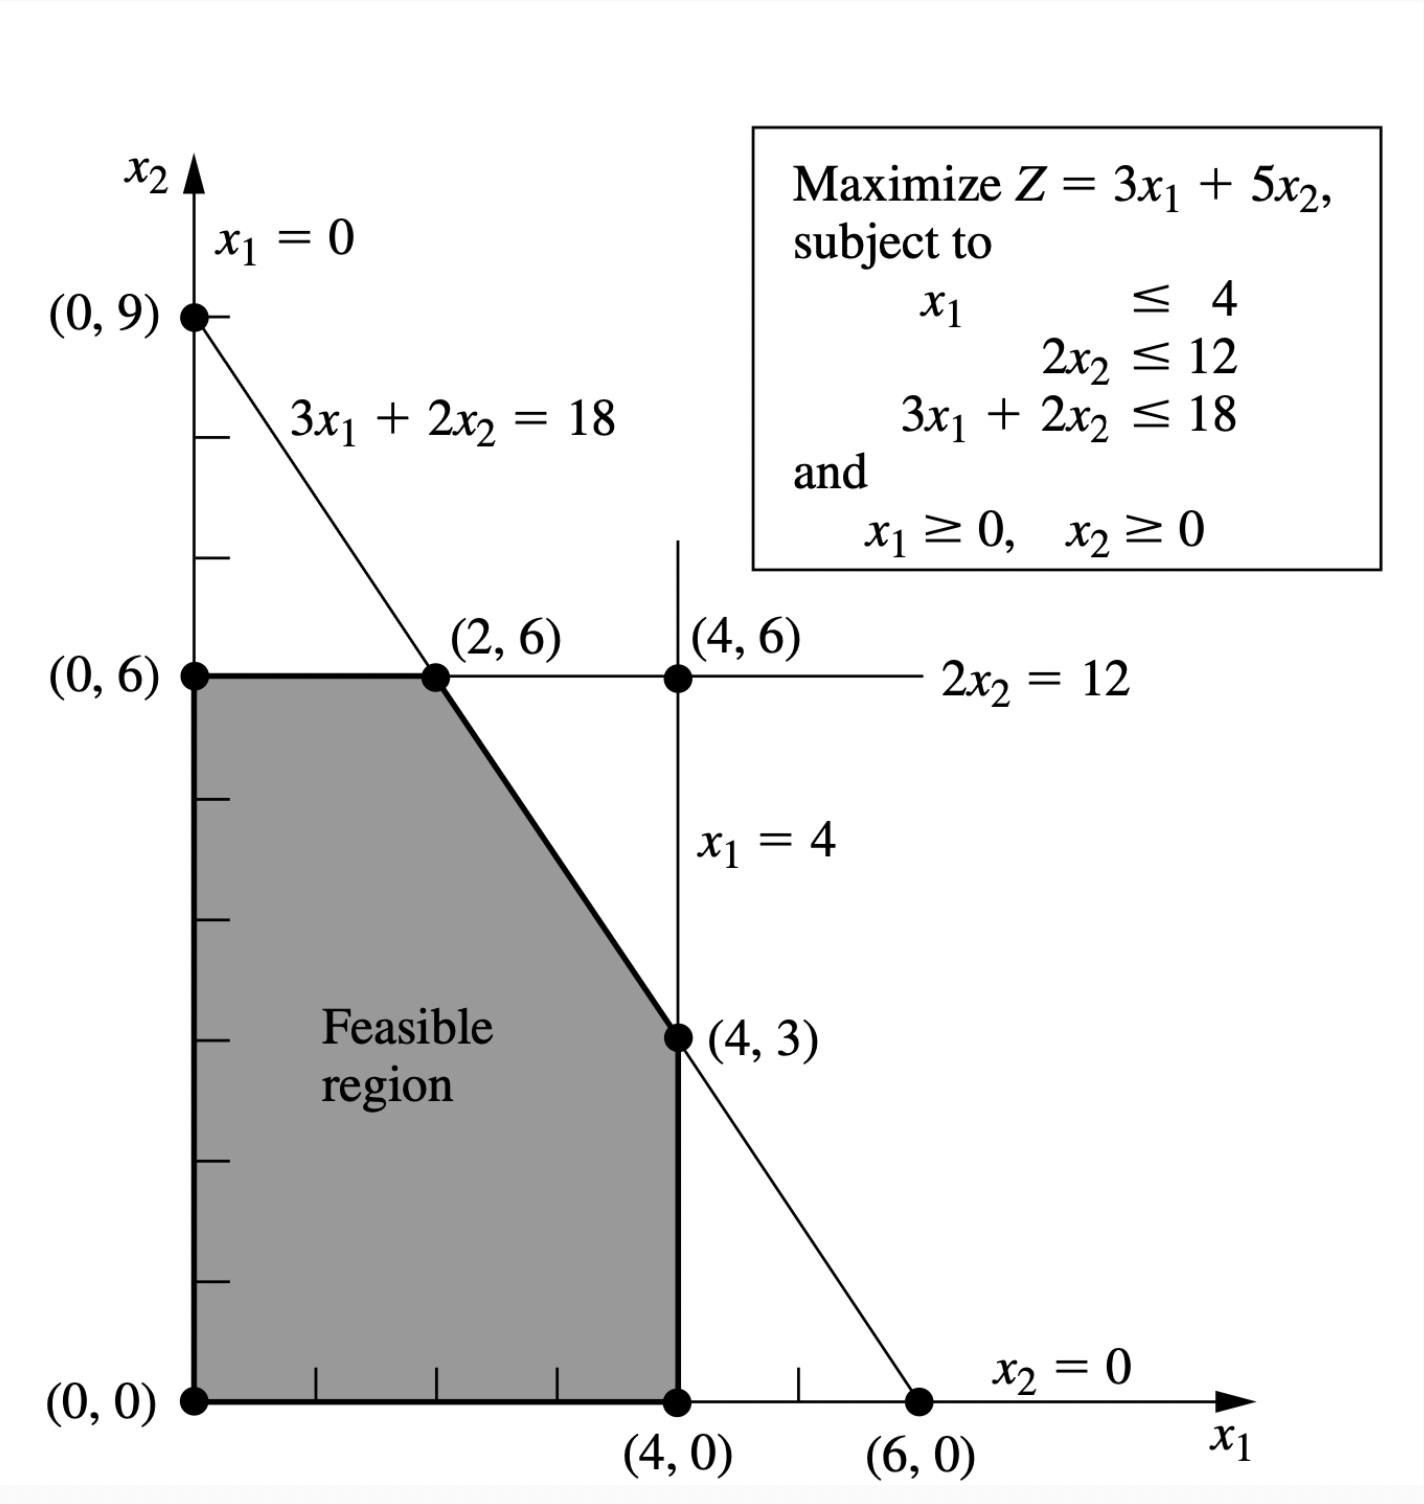
\includegraphics[width=0.5\textwidth]{Frontiera_vincolo_soluzioni_vertice.png}
    \caption{Problema 1}
    \label{fig:fig3}
\end{figure}

\vspace{1em}
\noindent
Per la determinazione della soluzione ottimale che massimizza la funzione obiettivo, sarà sufficiente individuare tutti i vertici della regione ammissibile (ponendo a $0$ di volta in volta $2$ variabili, che in $\mathbb{R}^2$ significa trovarsi su un vertice), per un totale di
\[\binom{5}{2} = 10\]
possibili soluzioni (anche se sono $8$ in quanto due vincoli paralleli) e calcolarne il corrispondente valore della funzione obiettivo:

\vspace{1em}
\noindent
\begin{table}[H]
    \rowcolors{1}{white}{white}
    \setlength{\tabcolsep}{8pt}
    \renewcommand{\arraystretch}{1.5}
    \noindent
    \centering
    \begin{tabular}{c|ccccc|c}
         & $x_1$ & $x_2$ & $s_1$ & $s_2$ & $s_3$ & $z$\\
        \hline
        $0$ & $0$ & $0$ & $4$ & $12$ & $18$ & $0$\\
        $A$ & $0$ & $4$ & $4$ & $0$ & $6$ & $30$\\
        $B$ & $2$ & $6$ & $2$ & $0$ & $0$ & $36$\\
        $C$ & $4$ & $3$ & $0$ & $6$ & $0$ & $27$\\
        $D$ & $4$ & $0$ & $0$ & $12$ & $6$ & $12$\\
        $E$ & $0$ & $3$ & $4$ & $-6$ & $0$ & $45$\\
        $F$ & $6$ & $0$ & $-2$ & $12$ & $0$ & $18$\\
        $G$ & $4$ & $6$ & $0$ & $0$ & $-4$ & $42$\\
    \end{tabular}
\end{table}

\vspace{1em}
\noindent
In cui, ovviamente, non possono essere considerate soluzioni ammissibili quelle in cui i coefficienti sono negative.

\vspace{1em}
\noindent
Si realizzi, ora, il duale di tale problema:
\begin{align*}
    \min w = 4 y_1 + 12 y_2 + 18 y_3\\
    y_1 + 3y_3 \geq 3\\
    2y_2 + 2y_3 \geq 5\\
    y_1,y_2,y_3 \geq 0
\end{align*}
che ridotto in forma standard diviene
\begin{align*}
    \min w = 4 y_1 + 12 y_2 + 18 y_3\\
    y_1 + 3y_3 - r_1 = 3\\
    2y_2 + 2y_3 - r_2 = 5\\
    y_1,y_2,y_3,r_1,r_2 \geq 0
\end{align*}
Avendo in questo caso $3$ variabili incognite e $2$ vincoli non è possibile prendere in considerazione la rappresentazione grafica di tale problema. Per trovare la soluzione ottimale si pongono di volta in volta a $0$, $3$ variabili (che in $\mathbb{R}^3$ significa trovarsi in un vertice del poliedro descritto), per un totale di
\[\binom{5}{3} = 10\]
anche se ovviamente non saranno tutte, in quanto alcune basi sono non ammissibili. Da ciò si evince che

\vspace{1em}
\noindent
\begin{table}[H]
    \rowcolors{1}{white}{white}
    \setlength{\tabcolsep}{8pt}
    \renewcommand{\arraystretch}{1.5}
    \noindent
    \centering
    \begin{tabular}{c|ccccc|c}
         & $y_1$ & $y_2$ & $y_3$ & $r_1$ & $r_2$ & $z$\\
        \hline
        $0$ & $0$ & $0$ & $0$ & $-3$ & $-5$ & $0$\\
        $A$ & $0$ & $\dfrac{5}{2}$ & $0$ & $-3$ & $6$ & $30$\\
        $B$ & $0$ & $\dfrac{3}{2}$ & $1$ & $0$ & $0$ & $36$\\
        $C$ & $-\dfrac{9}{2}$ & $0$ & $\dfrac{5}{2}$ & $0$ & $0$ & $27$\\
        $D$ & $3$ & $0$ & $0$ & $0$ & $-5$ & $12$\\
        $E$ & $0$ & $0$ & $\dfrac{5}{2}$ & $-\dfrac{3}{2}$ & $0$ & $45$\\
        $F$ & $0$ & $0$ & $1$ & $0$ & $-3$ & $18$\\
        $G$ & $\dfrac{3}{2}$ & $\dfrac{5}{2}$ & $0$ & $0$ & $0$ & $42$\\
    \end{tabular}
\end{table}

\vspace{1em}
\noindent
in cui è immediato osservare che esiste una corrispondenza tra la base originaria e la base duale ottenuta in questo caso, in quanto i valori della funzione obiettivo ottenuti nel problema primale corrispondono a quelli ottenuti nel problema duale.\\
Ovviamente le basi ammissibili, sia nel problema di partenza che in quello duale, sono tutte quelle in cui le variabili decisionali, comprese quelle fittizie, tutte non negative.\\
Ovviamente la soluzione ottimale del problema duale è $36$ per il teorema di dualità forte. Non solo, ma in corrispondenza del valore $36$ della funzione obiettivo esiste una base ammissibile sia per il problema primale che duale. Ad ogni base ammissibile del problema primale, invece, la corrispondente base duale è non ammissibile. Nell'esempio considerato, inoltre, esiste un solo caso in cui tanto una base del problema primale è non ammissibile, tanto è non ammissibile anche per il problema duale corrispondente.\\
Si osservi, inoltre, che per il problema primale di massimizzazione, sono ammissibili tutti i casi che sono minori della soluzione ottimale $36$. Tutti i casi in cui il valore della soluzione obiettivo è maggiore di $36$, a cui corrispondono basi non ammissibili per il problema primale, saranno ammissibili per il problema duale, in quanto essendo un problema di minimizzazione, si dovranno considerare soluzioni maggiori di quella ottimale, ossia maggiore di $36$.\\
Si ottiene, quindi, la schematizzazione seguente:

\vspace{1em}
\noindent
\begin{table}[H]
    \rowcolors{1}{white}{white}
    \setlength{\tabcolsep}{15pt}
    \renewcommand{\arraystretch}{1.5}
    \noindent
    \centering
    \begin{tabularx}{\textwidth}{@{}P@{}P|PP|@{}}
        && \multicolumn{2}{c}{Duale}\\
        && Ammissibile & Non Ammissibile\\
        \hline
        \multirow{2}{1em}{Primale} & Ammissibile &  \parbox{\linewidth}{\vspace{1em}\noindent Siamo nella soluzione ottima \vspace{1em}} &  \parbox{\linewidth}{\vspace{1em} \noindent Soluzione minore di $36$ \vspace{1em}}\\
        & Non Ammissibile &  \parbox{\linewidth}{Soluzione maggiore di $36$ \vspace{1em}} & \parbox{\linewidth}{I coefficienti non sono tutti non negativi per entrambi \vspace{1em}}\\
    \end{tabularx}
\end{table}

\vspace{1em}
\noindent
Le condizioni di complementarietà prevedono che date due variabili poste a $0$ nel problema primale, le corrispondenti variabili duali saranno non nulle e viceversa. Tali condizioni sono valide sempre, indipendentemente dal fatto che si considerino soluzioni di base ammissibili e non ammissibili.  

\vspace{1em}
\noindent
\textbf{Esercizio 2}: Si consideri il problema seguente
\begin{align*}
    & \max z = 4x_1 + 2x_2\\
    & 2x_1 \leq 16\\
    & x_1 + 3x_2 \leq 17\\
    & x_1 \leq 5\\
    & x_1,x_2 \geq 0\\
\end{align*}

\vspace{1em}
\noindent
È molto semplice realizzare graficamente tale problema, in cui è immediato evincere che la soluzione ottima è $C(8,3) \rightarrow 37$.\\
Si realizzi, ora, il problema duale corrispondente
\begin{align*}
    & \min w = 16 y_1 + 17y_2\\
    & 2y_1 +y_2 \geq 4\\
    & 3y_2 + y_3 \geq 2\\
    & y_1,y_2,y_3 \geq 0
\end{align*}

\vspace{1em}
\noindent
Ma è immediato evincere quale sia la base duale corrispondente alla funzione obiettivo. Siccome la soluzione ottimale nel problema primale non è sul vincolo $x_1 \leq 5$, ossia $s_3 > 0$, ciò significa che la corrispondente variabile decisionale duale $y_3=0$. Allora da ciò è facile capire dalle equazioni seguenti
\begin{align*}
    & 2y_1 +y_2 \geq 4\\
    & 3y_2 + y_3 \geq 2\\
\end{align*}
che i valori delle restanti variabili decisionali saranno
\[y_2 = \dfrac{2}{3} \hspace{1em} \text{e} \hspace{1em} y_1 = \dfrac{5}{3}\]
Ci si chiede, ora, quante unità supplementari della risorsa $1$ sono necessarie per aumentare di $15$ il valore di $z$. È noto che la funzione obiettivo $z$ vale $38$ in corrispondenza del valore $y_1^*=\dfrac{5}{3}$, ma si chiede che
\[53 = z = 35 + y_1* \cdot \underbrace{\Delta b_1}_{15}\]
Sapendo che il valore della variabili duale $y_1^*=\dfrac{5}{3}$, si ottiene che 
\[\dfrac{5}{3} \cdot \Delta b_1 = 15 \hspace{1em} \rightarrow \hspace{1em} \Delta b_1 = 9\]
per cui il primo vincolo di $\leq$ dovrà passare da $16$ a $16+9=25$.\\
Ovviamente, però, è fondamentale capire che non è possibile aumentare indefinitamente il primo vincolo, in quando quando non vi è più intersezione con il secondo, il primo diviene ridondante e quindi la variabile duale sarebbe $0$.\\
Spostando, quindi, a destra il primo vincolo, la nuova intersezione $C$ sarà data dall'intersezione del primo e del secondo vincolo, da cui
\begin{align*}
    &2x_1 = 25 & \rightarrow & x_1 = 12.5\\
    &x_2+3x_2 = 17 & \rightarrow & x_2 = 1.5
\end{align*}
e sostituendo nella funzione obiettivo i due valori trovati si ottiene $z= 4 \cdot 12.5 + 2 \cdot 1.5 = 53$, ossia il valore cercato.

\vspace{1em}
\noindent
\textbf{Osservazione}: Fondamentale osservare che la variabile duale $y_1$ vale $\dfrac{5}{3}$ solamente in un intorno di due intersezioni di vincoli, ossia quando il primo vincolo
\[4 \leq b_1 \leq 34\]
cioè persa la $x$ della intersezione a sinistra, ossia $B$, in cui $x=2$, si ha che $b_1=2x=4$, e tra l'intersezione del secondo vincolo obliquo con l'asse $x$ si ottiene $x=17$, per cui $b_1=2x=34$.

\newpage
\begin{center}
    11 Novembre 2022
\end{center}
\textbf{Esercizio 1}: Si consideri il problema di programmazione lineare formalizzato come segue
\begin{align*}
    &\max z = 2x_1 - 2x_2 - x_3\\
    &x_1 + x_2 + 2x_3 \leq 12\\
    &x_1+ x_2 -x_3 \leq 1\\
    &x_1,x_2,x_3 \geq 0
\end{align*}
Di fronte a tale problema si possono trovare due modalità di risoluzione
\begin{itemize}
    \item impiegare il metodo del simplesso, realizzando il tableau;
    \item essendo il problema con $3$ variabili e $2$ vincoli, il problema duale avrà $2$ variabili e $3$ vincoli.
\end{itemize}
Si sceglie, ovviamente, la seconda strada, per cui
\begin{align*}
    \min w = 12 y_1 + y_2\\
    y_1 + y_2 \geq 2\\
    y_1+y_2 \geq -2\\
    2y_1-y_2 \geq -1
\end{align*}
Si realizza la rappresentazione grafica dei vincoli e della funzione obiettivo, prestando attenzione ad individuare la corretta regione ammissibile. È facile capire che la regione ammissibile è infinita, in cui si individuano due vertici ammissibili
\[A=\left(\dfrac{1}{3},\dfrac{5}{3}\right) \hspace{1em} \text{e} \hspace{1em} B=(2,0)\]
a cui corrispondono i seguenti valori della funzione obiettivo
\[w_A=\dfrac{17}{3} \hspace{1em} \text{e} \hspace{1em} w_B=24\]
ovviamente il minimo si ha in $A$.\\
Per il teorema di dualità forte si ha che anche
\[z^*=\dfrac{17}{3}\]
per determinare, ora, i valori delle variabili decisionali delle variabili duali si usano le condizioni di complementarietà. Siccome si ha che $y_1 \neq 0$ e $y_2 \neq 0$ è immediato che le variabili di slack saranno $0$. Non solo, ma siccome la soluzione ottima del problema duale sta nell'intersezione dei vincoli $b_1$ e $b_3$, in cui le variabili di surplus saranno $=0$, da cui le variabili $x_1^*$ e $x_3^*$ saranno non nulle, mentre $x_2^*=0$. Ciò permette facilmente di risolvere il sistema seguente
\begin{align*}
    &x_1+ 2x_3 = 12\\
    &x_1-x_3 = 1\\
\end{align*}
che permette di ottenere $x_1=\dfrac{14}{3}$ e $x_2 = \dfrac{11}{3}$ che produce proprio il valore $x^*=\dfrac{17}{3}$.

\vspace{1em}
\noindent
\textbf{Esercizio 2}: Si consideri il problema formalizzato nel seguente modo:
\begin{align*}
    &\max z = 6x_1 + 8x_2\\
    &5x_1 + 2x_2 \leq 20\\
    &x_1 - 2x_2 \leq 10\\
    &x_1,x_2 \geq 0
\end{align*}
è immediato ricavare il duale
\begin{align*}
    &\min w = 20y_1 + 10y_2\\
    &5y_1 + y_2 \geq 6\\
    &2y_1 - 2y_2 \geq 8\\
    &y_1,y_2 \geq 0
\end{align*}
Realizzando graficamente i due problemi appena descritti si ottiene facilmente che nel problema primale vi sono in totale $6$ vertici, tra ammissibili e non ammissibili, così come nel problema duale, come ci si aspettava dal calcolo
\[\binom{4}{2}=6\]
in cui vi sono $2$ variabili decisionali e $2$ variali fittizie, con sempre $2$ vincoli.\\
Si ottiene la schematizzazione seguente:

\vspace{1em}
\noindent
\begin{table}[H]
    \rowcolors{1}{white}{white}
    \setlength{\tabcolsep}{8pt}
    \renewcommand{\arraystretch}{1.5}
    \noindent
    \centering
    \begin{tabular}{l|ccccc|ccccc|}
        Vertice & $x_1$ & $x_2$ & $s_1$ & $s_2$ & $z$ & $w$ & $y_1$ & $y_2$ & $r_1$ & $r_2$\\
        \hline
        $0$ & $0$ & $0$ & $10$ & $0$ & $0$ & $0$ & $0$ & $-4$ & $-6$\\
        $A$ & $0$ & $5$ & $10$ & $0$ & $40$ & $40$ & $0$ & $4$ & $-2$ & $0$\\
        $B$ & $\dfrac{5}{2}$ & $\dfrac{15}{4}$ & $0$ & $0$ & $45$ & $45$ & $\dfrac{1}{2}$ & $\dfrac{3}{2}$ & $0$ & $0$\\
        $C$ & $4$ & $0$ & $0$ & $6$ & $24$ & $24$ & $\dfrac{6}{5}$ &$0$ & $0$ & $-\dfrac{28}{5}$\\
        $D$ & $0$ & $10$ & $0$ & $-10$ & $80$ & $80$ & $4$ & $0$ & $14$ & $0$\\
        $E$ & $10$ & $0$ & $-30$ & $0$ & $60$ & $60$ & $0$ & $6$ & $0$ & $4$\\
    \end{tabular}
\end{table}
in cui per il primo problema, ovviamente, le basi ammissibili sono solamente le prime $4$.\\
Viceversa, per il problema duale, si avrà che le basi ammissibili per il primale saranno non ammissibili per il duale e viceversa (anche se potrebbero essere tutte e due non ammissibili). L'unica corrispondenza si avrà nel caso della soluzione ottima. Le condizioni di complementarietà sono:
\begin{align*}
    &x_1 r_1 = 0\\
    &x_2 r_2 = 0\\
    &s_1 y_1 = 0\\
    &s_2 y_2 = 0
\end{align*}
per cui se un fattore è $\neq 0$, l'altro dovrà essere $=0$ e viceversa.

\vspace{1em}
\noindent
\textbf{Esercizio 3}: Sia dato il problema seguente
\begin{align*}
    &\max z = 2x_1 - 7x_2 + 4x_3\\
    & x_2 + 2x_2 + x_2 \leq 10\\
    & 3x_1 + 3x_2 + 2x_3 \leq 10\\
    & x_1,x_2,x_3 \geq 0
\end{align*}
Si ottiene il problema duale seguente
\begin{align*}
    &\min w = 10y_1 + 10 y_2\\
    & y_1 + 3y_2 \geq 2\\
    & 2y_1 + 3y_2 \geq -7\\
    & y_1 + 2y_2 \geq 4\\
    & y_1,y_2 \geq 0
\end{align*}
Realizzando il grafico del problema duale si ottiene facilmente che il numero di vertici totali è
\[\binom{4}{3} = 4\]
Dovendo dimostrare che la soluzione ottima del problema primale deve essere $z^* \leq 25$, sarà sufficiente trovare una soluzione ammissibile del problema duale che vale $25$ (o anche meno); allora per dualità le soluzioni ammissibili del problema primale, compresa la soluzione ottima, dovranno essere $\leq 25$ (o comunque minore di ogni valore della funzione obiettivo del problema duale in corrispondenza di una base ammissibile).

\vspace{1em}
\noindent
\textbf{Esercizio 4}: Si consideri il problema seguente
\begin{align*}
    &\max z = x_1 + 2x_2\\
    &x_1 + 3x_2 \leq 8\\
    &x_1 - x_2 \leq 4\\
    &x_1,x_2 \geq 0
\end{align*}
Dalla rappresentazione grafica appare evidente che i vertici ammissibili trovati sono
\begin{align*}
    &A = \left(0,\dfrac{3}{5}\right) & \rightarrow & z=\dfrac{20}{3}\\
    &B=(2,2) & \rightarrow & z=6\\
    &C=(1,1) & \rightarrow & z=1
\end{align*}
Nell'ipotesi in cui il primo vincolo venga aumentato di $\delta_1=1$, mentre tutti gli altri vincoli rimangono costanti, per calcolare il prezzo ombra corrispondente, ossia il valore della variabile duale associata al primo vincolo, si ottiene che
\begin{align*}
    &x_1 + 3x_2 = 9\\
    &x_1 - x_2 = 4\\
\end{align*}
in cui si è potuto mettere il segno di $=$ in quando si è nell'intersezione di due vincoli, per cui $s_1$ e $s_2$ sono entrambi nulli. Si ottiene che $x_1=\dfrac{21}{4}$ e $x_2=\dfrac{5}{4}$.\\
Ne segue che, dato il problema duale
\begin{align*}
    &\min z = 8y_1 + 5y_2\\
    &y_1 + y_2 \geq 1\\
    &3y_1 - y_2 \geq 2\\
    &y_1,y_2 \geq 0
\end{align*}
Siccome $x_1 \neq 0$ e $x_2 \neq 0$, per le condizioni di complementarietà, segue che $r_1=0$ e $r_2=0$. È fa

\newpage
\begin{center}
    18 Novembre 2022
\end{center}
\subsection{Problemi di programmazione intera}
Per risolvere un problema di programmazione intera, non è possibile procedere tramite \textbf{enumerazione}, per cui vengono identificate tutte le soluzioni praticabili e viene scelta la migliore.\\
Ovviamente, tale processo potrebbe non essere praticabile. Per esempio, per risolvere il TSP (Travelling Salesman Problem) in un grafo completo con $n$ nodi ci sono $(n - 1)!$ tour fattibili. Quindi,

\vspace{1em}
\noindent
\begin{table}[H]
    \rowcolors{1}{white}{white}
    \setlength{\tabcolsep}{8pt}
    \renewcommand{\arraystretch}{1.5}
    \noindent
    \centering
    \begin{tabular}{c|c}
       $n$ & $n!$\\
       \hline
       $10$   & $3.6 \times 10^6$\\
       $100$  & $9.33 \times 10^{157}$\\
       $1000$ & $4.02 \times 10^{2567}$\\
    \end{tabular}
\end{table}
Per cui è opportuno trovare delle soluzioni migliori.

\vspace{2em}
\noindent
\textbf{Esempio}: Nel problema TSP (Travelling Salesman Problem) viene fornito un insieme di noti $\mathcal{V} = \{1,\dots,n\}$ che sarebbero le città e un insieme di archi $\mathcal{A}$. Gli archi rappresentano le coppie ordinate di città tra cui è possibile viaggiare direttamente.\\
Per $(i,j) \in \mathcal{A}$ si ha che $c_{i,j}$ è il tempo di percorrenza diretto dalla città $i$ alla città $j$.\\
Il problema TSP mira a trovare un tour, partendo dalla città $1$, che visiti ogni altra città esattamente una volta e poi ritorni alla città di partenza e impieghi il minor tempo di viaggio totale.

% Tabella per le definizione di concetti, etc...
\vspace{1em}
\rowcolors{1}{black!5}{black!5}
\setlength{\tabcolsep}{14pt}
\renewcommand{\arraystretch}{2}
\noindent
\begin{tabularx}{\textwidth}{@{}|P|@{}}
    \hline
    {\textbf{TRAVELLING SALESMAN PROBLEM (TSP)}}\\
    \parbox{\linewidth}{Un tour che visita tutti i nodi esattamente una volta è detto tour \textbf{hamiltoniano}. Il TSP identifica il tour hamiltoniano di costo minimo. \vspace{3mm}}\\
    \hline
\end{tabularx}

\vspace{1em}
\noindent
\subsubsection{Formulazione del TSP}
Le variabili decisionali sono
\[x_{i,j} = \left\{
    \rowcolors{1}{white}{white}
    \begin{array}{lll}
        1 & \text{se} & j \text{ segue immediatamente } i \text{ nel tour}\\
        0 & \text{altrimenti}
    \end{array}
\right.\]
per cui $x \in \{0,1\}^{\vert \mathcal{A} \vert}$. La funzione obiettivo, ovviamente, è
\[\min \sum_{(i,j) in \mathcal{A}} c_{i,j} \cdot x_{i,j}\]
Per quanto riguarda i vincoli, si deve richiedere che bisogna entrare e uscire da ogni città una e una sola volta, da cui
\begin{align*}
    &\sum_{i : (i,j) \in \mathcal{A}} x_{i,j} = 1 \hspace{1em} \forall j \in V\\
    &\sum_{j : (i,j) \in \mathcal{A}} x_{i,j} = 1 \hspace{1em} \forall i \in V\\
\end{align*}
Tuttavia, i vincoli di cui sopra non sono sufficienti a definire i tour, poiché sono soddisfatti anche dai sottocicli. Per eliminare i sottocicli, quindi, in ogni ciclo deve esserci un arco che va da $\{1,2,3\}$ al suo complementare $\{4,5,6\}$ e un arco che va da $\{4,5,6\}$ al suo complementare $\{1,2,3\}$. In generale, per qualsiasi $U \subseteq V$ con
\[2 \leq \vert U \vert \leq \vert V \vert - 2\]
i vincoli seguenti
\[\sum_{\{(i,j) \in \mathcal{A} : i \in U, j \in V-U\}} x_{i,j} \geq 1\]
sono soddisfatti da tutti i cicli, ma ogni sottociclo ne viola almeno uno, in quanto il numero di vincoli è molto elevato, dal momento che il numero di sottoinsiemi è $2^{\vert V \vert}$.\\
Un modo alternativo per eliminare i sottocicli è quello di introdurre vincoli
\[\sum_{\{(i,j) \in \mathcal{A} : i \in U, j \in U\}} x_{i,j} \leq \vert U \vert - 1 \hspace{1em} \forall U \subset V : 2 \leq \vert U \vert \leq \vert V \vert -2\]
Ma ancora una volta si necessita di un vincolo per ogni $U \subset V$ tale che $2 \leq \vert U \vert \leq \vert V \vert - 2$. Per qualunque formulazione dei vincoli, il numero dei vincoli è prossimo a $2^{\vert V \vert}$, o più precisamente
\[\dfrac{1}{2} \cdot \left[\binom{\vert V \vert}{2} + \binom{\vert V \vert}{3} + \dots + \binom{\vert V \vert}{\vert V \vert - 2} \right]\]

\vspace{1em}
\subsubsection{Risoluzione di un problema di programmazione intera}
Un modo per risolvere un problema di programmazione intera è quella di disattendere i vincoli di integrità delle variabili: non sapendo risolvere un problema di programmazione intera si considera tale problema come uno di programmazione continua.\\
Si consideri il seguente problema:
\begin{align*}
    &\max z = 1.00x_1 + 0.64x_2\\
    &50x_1 + 31x_2 \leq 250\\
    &3x_1 - 2x_2 \geq -4\\
    &x_1, x_2 \geq 0 \text{ interi}
\end{align*}
Allora
\begin{itemize}
    \item la soluzione ottimale intera è $(5,0)$;
    \item la soluzione ottimale senza considerare i vincoli di integrità delle variabili è
    \[\left(\dfrac{376}{193}, \dfrac{950}{193}\right) = (1.948, 4.922)\]
\end{itemize}
Ovviamente non è possibile utilizzare il simplesso per risolvere un problema di programmazione intera, in quanto la regione ammissibile non è un poliedro e non esiste nemmeno il concetto di vertice.

\begin{figure}[H]
    \centering
    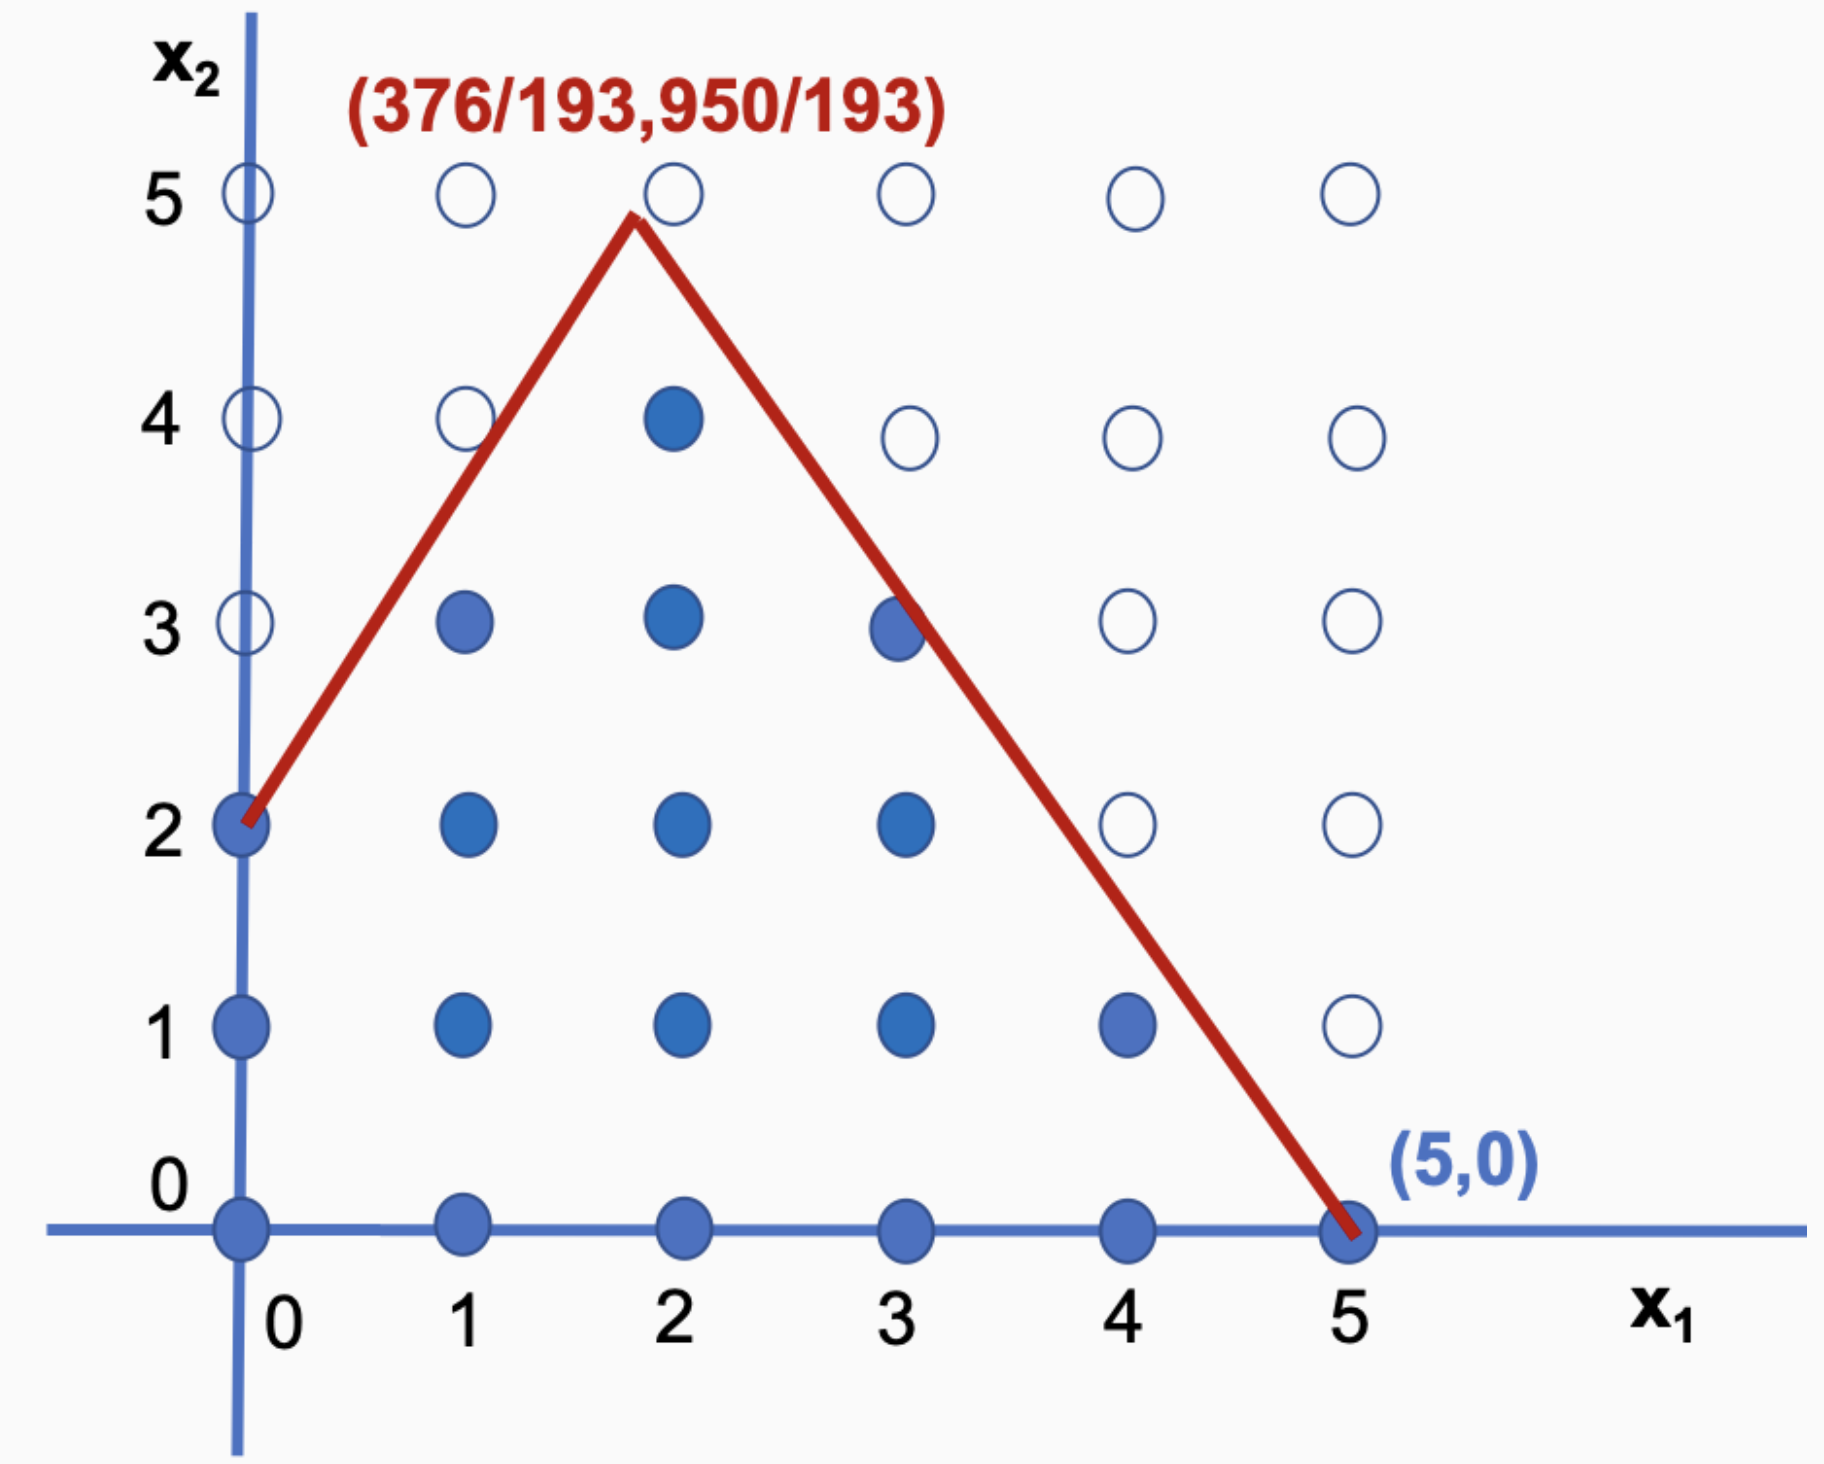
\includegraphics[width=0.5\textwidth]{problema-programmazione-intera.png}
    \caption{FRappresentazione di un problema di programmazione intera}
    \label{fig:fig2}
\end{figure}

\vspace{1em}
\noindent
Ci si potrebbe chiedere se non sia possibile arrotondare per eccesso e/o per difetto la soluzione lineare, in modo tale da ricondursi ad una soluzione intera
\begin{itemize}
    \item la parte intera superiore $(\lceil 1.948 \rceil,\lceil 4,922 \rceil) = (2, 5)$ non è ammissibile (il primo vincolo è violato);
    \item la parte intera inferiore $(\lfloor 1.948 \rfloor, \lfloor 4.922 \rfloor) = (1, 4)$ non è ammissibile (il secondo vincolo è violato);
    \item la scelta mista $(\rfloor 1.948 \lfloor, \lceil 4.922 \rceil) = (1, 5)$ non è ammissibile (il secondo vincolo è violato).
    \item la scelta mista $(\lceil 1.948 \rceil, \lfloor 4.922 \rfloor) = (2, 4)$ è ammissibile ma non ottima: $z(2, 4) = 4.56$, mentre $z(5, 0) = 5$. 
\end{itemize}
Non solo, nessun arrotondamento dà come risultato $z(5, 0)$, per cui, in conclusione, la soluzione lineare sembra essere inutile per trovare la soluzione intera.

\vspace{1em}
\subsubsection{Ottimalità}
Dato un problema di programmazione intera, come è possibile dimostrare che un dato punto $x^*$ è ottimale?\\
Tale domanda è fondamentale in quanto si è visto che l'enumerazione delle soluzioni potrebbe non essere possibile, mentre ignorare i vincoli di integrità delle variabili potrebbe non fornire informazioni utili.
Bisogna, quindi trovare delle alternative (cioè degli algoritmi) per risolvere un problema di programmazione intera.

\vspace{1em}
\subsubsection{Limiti}
L'approccio più comune per risolvere i problemi di programmazione intera è quello di trovare sequenze di limiti fino a quando non sono \quotes{abbastanza vicini}, per cui si definisce

% Tabella per le definizione di concetti, etc...
\vspace{1em}
\rowcolors{1}{black!5}{black!5}
\setlength{\tabcolsep}{14pt}
\renewcommand{\arraystretch}{2}
\noindent
\begin{tabularx}{\textwidth}{@{}|P|@{}}
    \hline
    {\textbf{LIMITE SUPERIORE}}\\
    \parbox{\linewidth}{Se $z$ è il valore ottimo di un problema di progrmmazione intera, un limite superiore è un valore $\overline{z}$ tale che $\overline{z} \geq z$. \vspace{3mm}}\\
    \hline
\end{tabularx}

% Tabella per le definizione di concetti, etc...
\vspace{1em}
\rowcolors{1}{black!5}{black!5}
\setlength{\tabcolsep}{14pt}
\renewcommand{\arraystretch}{2}
\noindent
\begin{tabularx}{\textwidth}{@{}|P|@{}}
    \hline
    {\textbf{LIMITE INFERIORE}}\\
    \parbox{\linewidth}{Se $z$ è il valore ottimo di un problema di progrmmazione intera, un limite inferiore è un valore $\underline{z}$ tale che $\underline{z} \leq z$. \vspace{3mm}}\\
    \hline
\end{tabularx}

\vspace{1em}
\noindent
Idealmente, si vorrebbe trovare $\overline{z}$ e $\underline{z}$ tali che $\underline{z} = z = \overline{z}$.\\
Da un punto di vista meramente pratico, qualsiasi algoritmo cercherà una sequenza decrescente di limiti superiori
\[\overline{z_1} > \overline{z_2} > \dots > \overline{z_s} \geq z\]
e una sequenza crescente di limiti inferiori 
\[\underline{z_1} < \underline{z_2} < \dots < \underline{z_t} \leq z\]
e ci si ferma quando
\[\overline{z_s} - \underline{z_t} \leq \epsilon\]
dove $\epsilon$ è un valore appropriato non negativo.

\vspace{2em}
\noindent
\textbf{Osservazione 1}: Si osservi che ogni soluzione ammissibile $\hat x \in X$ fornisce un limite inferiore (o primale) $z = c(\hat x) \leq z$.\\
Per il problema
\begin{align*}
    &\max z = 1.00x_1 + 0.64x_2\\
    &50x_1 + 31x_2 \leq 250\\
    &3x_1 - 2x_2 \geq -4\\
    &x_1, x_2 \geq 0 \text{ interi}
\end{align*}
si è visto che arrotondando la soluzione lineare ottimale, ossia $\hat x = (2, 4)$ è una soluzione ammissibile tale che $z = c(\hat x) = 4.56 \leq z$.

\vspace{2em}
\noindent
\textbf{Osservazione 2}: La ricerca di limiti superiori potrebbe essere meno ovvia. L'idea più comune è quella di sostituire un problema di programmazione intera \quotes{difficile} con un problema di ottimizzazione più semplice, il cui valore ottimale sia almeno pari a $z$. Il problema più semplice può essere ottenuto con un \quotes{\textbf{rilassamento}}, cioè 
\begin{itemize}
    \item allargando l'insieme delle soluzioni ammissibili in modo da ottimizzare su un insieme più ampio;
    \item sostituendo la funzione obiettivo con una funzione che abbia ovunque lo stesso valore o un valore maggiore.
\end{itemize}

% Tabella per le definizione di concetti, etc...
\vspace{1em}
\rowcolors{1}{black!5}{black!5}
\setlength{\tabcolsep}{14pt}
\renewcommand{\arraystretch}{2}
\noindent
\begin{tabularx}{\textwidth}{@{}|P|@{}}
    \hline
    {\textbf{RILASSAMENTO}}\\
    \parbox{\linewidth}{Un problema
    \[(RP) x^R = \max \{f(x) : x \in T \subseteq \mathbb{R}^n\}\]
    è un \textbf{problema di rilassamento} di
    \[(IP)z = \max \{c(x) :  x \in X \subseteq \mathbb{Z}^n\}\]
    se
    \begin{itemize}
        \item $X \subseteq T$;
        \item $f(x) \geq c(x) \hspace{1em} \forall x \in X$.
    \end{itemize}
    \vspace{1mm}}\\
    \hline
\end{tabularx}

\vspace{1em}
In questo modo, se $x^*$ è la soluzione ottimale di un problema di programmazione intera, xon $x^* \in X \subseteq T$ e con $x = c(x^*) \leq f(x^*)$; pertanto, come $x^* \in T$, allora $f(x^*)$ è un limite inferiore per $x^R$, e quindi
\[z \leq f(x^*) \leq z^R\]
per cui $z^R$ è un limite superiore.

\vspace{1em}
\subsubsection{Rilassamento lineare}
Per programma intero
\[\max\{cx : x \in X = P \cap \mathbb{Z}^n\}\]
con formulazione
\[P = \{x \in \mathbb{R}_+^n : Ax \leq b\}\]
il \textbf{rilassamento di programmazione lineare} è il programma lineare
\[z^{LP} = \max\{cx : x \in P\}\]
Poiché $X = P \cap \mathbb{Z}^n \subseteq P$ e la funzione obiettivo è invariata, si tratta chiaramente di un rilassamento.

\vspace{2em}
\noindent
\textbf{Esempio 1}: Si consideri il seguente esempio di rilassamento
\begin{align*}
    & \text{Problema di programmazione intera originario} & & \text{Rilassamento lineare}\\
    &\max z = 1.00x_1 + 0.64x_2 && \max z^{LP} = 1.00x_1 + 0.64x_2\\
    &50x_1 + 31x_2 \leq 250 && 50x_1 + 31x_2 \leq 250\\
    &3x_1 - 2x_2 \geq -4 && 3x_1 - 2x_2 \geq -4\\
    &x_1, x_2 \geq 0 \text{ interi} &&x_1, x_2 \geq 0
\end{align*}
Allora, per quanto osservato, si ha che
\begin{itemize}
    \item la soluzione intera ottimale è $(5, 0)$ e $z = 5$;
    \item La soluzione ottimale del rilassamento lineare è \[\left(\dfrac{376}{193}, \dfrac{950}{193}\right) \hspace{1em} \text{e} \hspace{1em} z^{LP} = \dfrac{948}{193} = 5.098\]
\end{itemize}
Allora è noto che il limite inferiore è $\underline{z} = 4.560$ e il limite superiore è $\overline{z}=5.098$. Il valore ottimale $z$ è quindi compreso tra
\[\underline{z} = 4.560 \leq z \leq 5.098 = \overline{z}\]
In effetti, $z = 5$. Le informazioni che si ottengono trascurando i vincoli di integrità delle variabili possono essere, quindi, davvero molto utili.

\vspace{2em}
\textbf{Esempio 2}: Si consideri il seguente problema di programmazione intera
\begin{align*}
    &z=\max 4x_1 - x_2\\
    &7x_1 - 2x_2 \leq 14\\
    &x_2 \leq 3\\
    &2x_1 - 2x_2 \leq 3\\
    &x_1, x_2 \geq 0 \text{ interi}
\end{align*}
È facile vedere che $(2,1)$ è una soluzione ammissibile, e quindi si ottiene il limite inferiore $\underline{z}=7$. La soluzione ottimale del rilassamento lineare è $x^* = \left(\dfrac{20}{7},3\right)$ che produce il limite superiore $\overline{z} = \dfrac{59}{7} = 8.43$.\\
Poiché \textbf{tutti i coefficienti della funzione obiettivo sono interi} (cioè $(4,-1)$), anche il valore ottimale $z$ deve essere intero. Quindi, è possibile considerare come limite superiore $\overline{z} = \lfloor 8,43 \rfloor = 8$. Quindi
\[\underline{z}=7 \leq z \leq 8 = \overline{z}\]
\end{document} 